
\documentclass[11pt,a4paper,fleqn,openany]{report}

\usepackage{analysis_3_sty}
%% Headers and Footers
\fancyhf[LH]{inoffizielles Skript\\von Lars Gavris}
\fancyhf[CH]{Analysis 3}
\fancyhf[RH]{SS20/21\\Prof. Lamm}

\begin{document}
  \sidenote{Vorlesung 1}{02.11.2020}
  % 
  % Vorwort
  % 
  \begin{goals}
    \begin{enumerate}
      \item[]
      \item Maßtheorie $\to$ Lebesgue-Maß\\(Volumen von Teilmengen des $\mathbb{R}^n$ bestimmen)
      \item Integralrechnung für Funktionen $f:\Omega \subseteq \mathbb{R}^n \to \mathbb{R}$\\$\to$ Lebesgue-Integrale (Satz von Fubini, ...)
      \item Version des Hauptsatzes $\to$ Satz von Gauß 
    \end{enumerate}
  \end{goals}

  \chapter{Maße und messbare Funktionen}

  \begin{notation}
    Menge $X$, Potenzmenge $\script{P}(X)$, eine Teilmenge von $\script{P}(X)$ heißt Mengensystem
  \end{notation}

  \begin{definition}
    Ein Mengensystem $\script{A} \subseteq \script{P}(X)$ heißt \textbf{$\bm{\sigma}$-Algebra}, falls:
    \begin{enumerate}[label=(\roman*)]
      \item $X \in \script{A}$
      \item $A \in \script{A} \implies X \setminus A \in \script{A}$
      \item $A_i \in \script{A}, \forall i \in \mathbb{N} \implies \bigcup\limits_{i \in \mathbb{N}} A_i \in \script{A}$
    \end{enumerate}
    Das Paar $(X, \script{A})$ heißt dann \textbf{messbarer Raum}.
  \end{definition}

  \begin{remark}
    \begin{enumerate}
      \item[]
      \item $A_i \in \script{A}, \forall i \in \mathbb{N} \implies \bigcap\limits_{i \in \mathbb{N}} A_i \in \script{A}$\\
            Denn: $\bigcap\limits_{i \in \mathbb{N}} A_i = X \setminus (\bigcup\limits_{i \in \mathbb{N}} X \setminus A_i)$
      \item $\emptyset = X \setminus X \in \script{A}$
      \item $A,B \in \script{A} \implies A \setminus B \in \script{A}$\\
            Denn: $A \setminus B = A \cap (X \setminus B)$
    \end{enumerate}
  \end{remark}

  \begin{example}
    \begin{enumerate}
      \item[]
      \item $\script{P}(X)$ ist $\sigma$-Algebra, $\{\emptyset, X\}$ ist $\sigma$-Algebra
      \item später: Menge aller messbaren Mengen eines äußeren Maßes bildet eine $\sigma$-Algebra.
    \end{enumerate}
  \end{example}
  
  \begin{theorem}
    Jeder Durchschnitt von (endlich oder unendlich vielen) $\sigma$-Algebren auf der selben Menge $X$ ist wieder eine $\sigma$-Algebra.
  \end{theorem}

  \begin{proof}
    $(A_i)_{i \in I}$ sei eine Familie von $\sigma$-Algebren bezüglich $X$.\\
    Offensichtlich gilt: $X \in \bigcap\limits_{i \in I} \script{A}_i$\\
    Sei $A \in \bigcap\limits_{i \in I} \script{A}_i \implies A \in \script{A}_i \ \forall i \in I \implies X \setminus A \in \script{A}_i \ \forall i \in I \implies X \setminus A \in \bigcap\limits_{i \in I} A_i$\\
    Analog für die abzählbare Vereinigung.
  \end{proof}

  \begin{definition}
    Für ein Mengensystem $\script{E} \subseteq \script{P}(X)$ heißt $\sigma(\script{E}) := \bigcap\{\script{A}|\script{A}$ ist $\sigma$-Algebra in $X$ mit $\script{E} \subseteq \script{A}\}$ die von $\script{E}$ \textbf{erzeugte $\bm{\sigma}$-Algebra}. Man nennt $\script{E}$ das \textbf{erzeugende System} von $\sigma(\script{E})$.
  \end{definition}

  \begin{remark}
    Dieser Durchschnitt ist nicht-trivial, denn $\script{P}(X)$ ist $\sigma$-Algebra mit $\script{E} \subseteq \script{P}(X)$.
  \end{remark}

  \begin{example}
    \begin{enumerate}
      \item[]
      \item Ist $E \subseteq X$ und $\script{E} = \{E\} \implies \sigma(\script{E}) = \{\emptyset, E, X \setminus E, X\}$
      \item Sei $(X,d)$ ein metrischer Raum. $\script{O} \subseteq \script{P}(X)$ sei das System der offenen Mengen. Die von $\script{O}$ erzeugte $\sigma$-Algebra heißt \textbf{Borel-$\bm{\sigma}$-Algebra} $\mathbb{B} (\script{O})=\mathbb{B}$. Ihre Elemente heißen \textbf{Borelmengen}.
      \item Seien $X \neq \emptyset$, $(Y, \script{C})$ messbarer Raum, $f:X \to Y$ eine Abbildung und das Urbild von $C \subseteq Y$: $f^{-1}(C) := \{x \in X|f(x) \in C\}$. Dann ist $f^{-1}(\script{C}):=\{f^{-1}(C)|C \in \script{C}\}$ eine $\sigma$-Algebra bzgl. $X$.\\
            Begründung: 
            \begin{itemize}
              \item $X \in f^{-1}(\script{C})$, denn $f^{-1}(Y) = X$ und $Y \in \script{C}$
              \item $f^{-1}(C) \in f^{-1}(\script{C}) \iff C \in \script{C}$,\\$f^{-1}(Y \setminus C) = X \setminus f^{-1}(C)$
              \item Erinnerung: $f^{-1}(A \cup B) = f^{-1}(A) \cup f^{-1}(B)$
            \end{itemize}
      \item Sei $X$ eine beliebige Menge und $\script(E)_i \subseteq \script{P}(X)$, $i \in I$, Mengensysteme, dann gilt: $\sigma(\bigcup\limits_{i \in I} \script{E}_i) = \sigma(\bigcup\limits_{i \in I} \sigma(\script{E}_i))$\\
            Begründung:
            \begin{itemize}
              \item Klar: $\subseteq$
              \item Andererseits enthält $\sigma(\bigcup\limits_{i \in I} \script{E}_i)$ das System $\bigcup\limits_{i \in I} \sigma (\script{E}_i)$ und ist eine $\sigma$-Algebra $\implies \sigma(\bigcup\limits_{i \in I} \sigma(\script{E}_i)) \subseteq \sigma(\bigcup\limits_{i \in I} \script{E}_i)$
            \end{itemize}
    \end{enumerate}
  \end{example}

  \begin{notation}
    $\bar{\mathbb{R}} := \mathbb{R} \cup \{+\infty, -\infty\}$ mit $-\infty < a < +\infty,\ \forall a \in \mathbb{R}$
  \end{notation}

  \newpage

  \begin{definition}
    Eine Folge $(s_k) \subseteq \bar{\mathbb{R}}\ (k \in \mathbb{N})$ konvergiert gegen $s \in \bar{\mathbb{R}}$, falls eine der folgenden Alternativen gilt:
    \begin{enumerate}[label=(\roman*)]
      \item $s \in \mathbb{R}$ und $\forall \epsilon>0$ gilt: $s_k \in (s-\epsilon, s+\epsilon) \subseteq \mathbb{R}$ für k hinreichend groß
      \item $s=\infty$ und $\forall r \in \mathbb{R}: s_k \in (r, \infty]$ für k hinreichend groß
      \item $s=-\infty$ und $\forall r \in \mathbb{R}: s_k \in [-\infty, r)$ für k hinreichend groß
    \end{enumerate}
    $(s_k) \subseteq \mathbb{R}$ ist genau dann in $\bar{\mathbb{R}}$ konvergent, wenn sie entweder in $\mathbb{R}$ konvergiert, oder bestimmt gegen $\pm\infty$ divergiert.
  \end{definition}

  \begin{example}
    \begin{itemize}
      \item[]
      \item $s_k$ monoton $\implies\ s_k$ konvergiert in $\bar{\mathbb{R}}$
      \item $a_k \geq 0 \implies \sum\limits_{k \in \mathbb{N}}a_k \in \bar{\mathbb{R}}$
      \item Eine Menge $U \subseteq \bar{\mathbb{R}}$ ist genau dann offen, wenn $U \cap \mathbb{R}$ offen ist und im Fall $+\infty \in U$ (bzw. $-\infty \in U$) ein $a \in \mathbb{R}$ existiert, sodass $(a,\infty] \subseteq U$ (bzw. $[-\infty,a) \subset U$) ist.
      \item Die Borel-$\sigma$-Algebra $\bar{\mathbb{B}}$ auf $\bar{\mathbb{R}}$ wird durch die offenen Mengen in $\bar{\mathbb{R}}$ erzeugt. Es gilt: $\bar{\mathbb{B}} = \{B \cup E|B \in \mathbb{B}, E \subseteq \{-\infty,+\infty\}\}$ 
    \end{itemize}
  \end{example}

  \begin{notation}
    \underline{Addition:}
    \begin{tabular}[t]{c | c c c}
      + & $-\infty$ & $\mathbb{R}$ & $+\infty$\\
      \hline
      $-\infty$ & $-\infty$ & $-\infty$ & /\\
      $\mathbb{R}$ & $-\infty$ & $\mathbb{R}$ & $+\infty$\\
      $+\infty$ & / & $+\infty$ & $+\infty$
    \end{tabular}\\
    $\sup\emptyset := -\infty,\ \inf\emptyset := +\infty$ konsistent mit $A,B \subseteq \mathbb{R}$ gilt $A \subseteq B \implies \sup A < \sup B$ und $\inf A \geq \inf B$ 
  \end{notation}

  \begin{definition}
    Sei $\script{A} \subseteq \script{P}(X)$ eine $\sigma$-Algebra, eine nicht-negative Mengenfunktion $\mu: \script{A} \rightarrow [0, \infty]$ heißt \textbf{Maß} auf $\script{A}$, falls:
    \begin{enumerate}[label=(\roman*)]
      \item $\mu(\emptyset) = 0$
      \item für beliebige paarweiße disjunkte $A_i \in \script{A}$, $i \in \mathbb{N}$, gilt:\\
            $\mu(\bigcup\limits_{i \in \mathbb{N}} A_i) = \sum\limits_{i \in \mathbb{N}} \mu (A_i)$ \hfill ($\sigma$-Additivität)
    \end{enumerate}
    Das Tripel $(X, \script{A}, \mu)$ heißt \textbf{Maßraum}.
  \end{definition}

  \begin{remark}
    \begin{enumerate}
      \item[]
      \item Für endlich viele paarweiße disjunkte $A_i \in \script{A}$, $i=1,...,n$, folgt aus (ii) indem man $A_i=\emptyset$ für $i=n+1, ...$ setzt: $\mu(\bigcup\limits_{i=1}^n A_i) = \sum\limits_{i=1}^n \mu(A_i)$
      \item Monotonie des Maßes: $A,B \in \script{A}$ mit $A \subseteq B \implies \mu(A) \leq \mu(B) = \mu(A \cup (B \setminus A)) = \mu(A) + \mu(B \setminus A)$
    \end{enumerate}
  \end{remark}

  \begin{definition}
    Sei $(X, \script{A}, \mu)$ ein Maßraum. Das Maß $\mu$ heißt \textbf{endlich}, wenn $\mu(A) < \infty\ \forall A \in \script{A}$ und $\bm{\sigma}$\textbf{-endlich}, wenn es eine Folge $(X_i) \in \script{A}$ mit $\mu(X_i) < \infty$ gibt, sodass $X=\bigcup\limits_{i \in \mathbb{N}} X_i$. Falls $\mu(X) = 1$, so wird $\mu$ \textbf{Wahrscheinlichkeits-Maß} genannt.
  \end{definition}

  \begin{example}
    \begin{enumerate}
      \item[]
      \item Sei $X$ eine beliebige Menge, $\script{A} = \script{P}(X)$, für $x \in X$ sei $\delta_x(A) := \begin{cases}1, & x \in A\\0, & x \notin A\end{cases}$ (\textbf{Dirac-Maß})
            \begin{itemize}
              \item Es gilt $\delta_x(A) \in \{0,1\}$, $\delta_x(\emptyset) = 0$, $\delta_x(X) = 1$.
              \item Sei $A = \bigcup\limits_{k \in \mathbb{N}} A_k$ gegeben mit $A_k$ paarweiße disjunkt und $x \in A \implies x \in A_k$ für genau ein $k \in \mathbb{N} \implies\ \sigma$-Additivität.
              \item Für $x \notin A$ gilt sowieso $\delta_x{A} = 0$
            \end{itemize}
            $\implies$ Das Dirac-Maß ist ein Wahrscheinlichkeits-Maß
      \item \textbf{Zählmaß:} $X$ beliebige Menge \sidenote{Vorlesung 2}{06.11.2020}\\
            $card: \script{P}(X) \to [0, \infty]$\\
            $card(A) := \begin{cases}\text{Anzahl der Elemente von A}, & \text{falls A endlich}\\\infty, sonst\end{cases}$\\
            Für $A = \bigcup\limits_{k\in \mathbb{N}}A_k$ endlich und paarweiße disjunkt ist die $\sigma$-Additivität klar.\\
            \\
            Sei $A$ unendlich und $A = \bigcup\limits_{k\in \mathbb{N}}A_k$.
            \begin{enumerate}
              \item nur endlich viele $A_k$ nicht-trivial\\
                    $\implies \exists k_0: A_{k_0}$ ist unendlich
              \item abzählbar viele $A_k$ sind nicht-trivial $\implies$ Behauptung
            \end{enumerate}
            $\implies$ Behauptung\\
            \\
            Zählmaß ist $\sigma$-endlich $\Leftrightarrow X$ ist abzählbar\\
            Zählmaß ist endlich $\Leftrightarrow X$ ist endlich
    \end{enumerate}
  \end{example}

  \begin{example}
    $X$ beliebige Menge, $\script{A} \subseteq \script{P}(X)$ $\sigma$-Algebra, $\mu(A)=0 \ \forall A \in \script{A}$
  \end{example}

  \begin{theorem}[Stetigkeitseigenschaften von Maßen]
    Sei $(X,\script{A},\mu)$ Maßraum. Dann gelten für Mengen $A_i \in \script{A}, i \in \mathbb{N}$ folgende Aussagen:

    \begin{enumerate}[label=(\roman*)]
      \item Aus $A_1 \subseteq A_2 \subseteq A_3 \subseteq ...$ folgt: $\mu (\bigcup\limits_{i \in \mathbb{N}} A_i) = \lim\limits_{i \to \infty} \mu (A_i)$
      \item Aus $A_1 \supseteq A_2 \supseteq A_3 \supseteq ...$ mit $\mu(A_1)<\infty$, folgt: $\mu (\bigcap\limits_{i \in \mathbb{N}} A_i) = \lim\limits_{i\to \infty} \mu (A_i)$
      \item $\mu(\bigcup\limits_{i\in \mathbb{N}} A_i) \leq \sum\limits_{i\in \mathbb{N}} \mu(A_i)$
    \end{enumerate}
  \end{theorem}

  \begin{remark}
    \begin{enumerate}
      \item[]
      \item \begin{enumerate}[label=(\roman*)]
        \item Stetigkeit von unten
        \item Stetigkeit von oben
        \item $\sigma$-Subadditivität von $\mu$
      \end{enumerate}
      \item Bedingung $\mu(A_i) \leq \infty$ in (ii) kann durch $\mu(A_k) \leq \infty$ für ein $k \in \mathbb{N}$ ersetzt werden, kann aber nicht weggelassen werden.\\
            Begründung:\\
            $A_k = {k, k+1,...} \subseteq \mathbb{N}$\\
            $card(A_k) = \infty \ \forall k \in \mathbb{N}$\\
            Aber: $card(\bigcap\limits_{i \in \mathbb{N}} A_i) = card(\emptyset) = 0$ 
    \end{enumerate}
  \end{remark}

  \begin{proof}
    \begin{enumerate}[label=(\roman*)]
      \item[]
      \item $\tilde{A_1} := A_1, \ \tilde{A_k} := A_k \setminus A_{k-1}, \ k \geq 2$\\
            $\tilde{A_i}$ sind paarweiße disjunkt.\\
            $\bigcup\limits_{i \in \mathbb{N}} \tilde{A_i} = \bigcup\limits_{i \in \mathbb{N}} A_i$\\
            $\mu(\bigcup\limits_{i \in \mathbb{N}} A_i) = \mu(\bigcup\limits_{i \in \mathbb{N}} \tilde{A_i}) = \sum\limits_{i \in \mathbb{N}} \mu(\tilde{A_i}) = \lim\limits_{k \to \infty}(\sum\limits_{i=1}^k \mu(\tilde{A_i})) = \lim\limits_{k \to \infty} \mu(\bigcup\limits_{i=1}^k A_k) = \lim\limits_{k \to \infty} \mu(A_k)$
      \item $A'_k := A_1 \setminus A_k \ \implies \ A'_1 \subseteq A'_2 \subseteq ...$\\
            Es gilt: $\mu(A_1) = \mu(A_1 \cap A_k) + \mu(A_1 \setminus A_k) = \mu(A_k) + \mu(A'_k)$\\
            $\implies \mu(A_1) - \lim\limits_{k \to \infty} \mu(A_k) = \lim\limits_{k \to \infty} \mu(A'_k) \stackrel{(i)}{=} \mu(\bigcup\limits_{k \in \mathbb{N}} A'_i) = \mu(A_1 \setminus \bigcap\limits_{i \in \mathbb{N}})\\ = \mu(A_1) - \mu(\bigcap\limits_{i \in \mathbb{N}} A_i)$
      \item Es genügt, die Folge $B_1 = A_1,\ B_i \stackrel{i \geq 2}{=} A_i \setminus \bigcup\limits_{j=1}^{i-1}A_j$ zu betrachten.\\
            $\bigcup\limits_{i \in \mathbb{N}} A_i = \bigcup\limits_{i \in \mathbb{N}} B_i$ und $(B_i)$ ist paarweiße disjunkt.\\
            $\implies \mu(\bigcup\limits_{i \in \mathbb{N}} A_i) = \mu(\bigcup\limits_{i \in \mathbb{N}} B_i) = \sum\limits_{i \in \mathbb{N}} \mu(B_i) \leq \sum\limits_{i \in \mathbb{N}} \mu(A_i)$
    \end{enumerate}
  \end{proof}

  \begin{definition}
    $(X, \script{A}, \mu)$ Maßraum.\\
    Jede Menge $A \in \script{A}$ mit $\mu(A) = 0$ heißt $\bm{\mu}$\textbf{-Nullmenge}. Das System aller $\mu$-Nullmengen bezeichnen wir mit $\bm{\script{N}(\mu)}$. Das Maß $\mu$ heißt \textbf{vollständig}, wenn gilt:\\
    \[
      N \subseteq A \text{ für ein } H \in \script{A} \text{ mit } \mu(A)=0\\
      \implies N \in \script{A} \text{ und } \mu(N)=0
    \]
  \end{definition}

  \begin{remark}
    Nicht jedes Maß ist vollständig:
    \[
      \script{A} \neq \script{P}(X) \ \mu(A) = 0 \ \forall A \in \script{A}
    \]
    Allerdings lässt sich jedes Maß vervollständigen:\\
    Sei $(X, \script{A}, \mu)$ Maßraum und $\script{T}_{\mu}$ sei das System aller Mengen $N \subseteq X$ für die keine $\mu$-Nullmenge $B \in \script{N}(\mu)$ existiert mit $N \subseteq B$. Es gilt:\\
    \[
      \mu \text{ vollständig } \Leftrightarrow \script{T}_{\mu} \subseteq \script{A}
    \]
    Definiere auf $\bar{A_{\mu}} := \{A \cup N | A \in \script{A}, N \in \script{T}_{\mu}\}$ die Mengenfunktion $\bar{\mu}$ durch $\bar{\mu}(A\cup N) := \mu(A) \ \forall A \in \script{A}, N\in \script{T}_{\mu}$
  \end{remark}

  \begin{remark}
    $\bar{\mu}$ ist wohldefiniert: $A \cup N = B \cup P$ mit $A,B\in \script{A}, \ P,N \in \script{T}_{\mu} \implies \exists C \in \script{A}, \mu(C) = 0: P \subseteq C \implies A \subseteq B \cup C \implies \mu(A) \leq \mu(B) + \mu(C) = \mu(B)$\\
    Symm $\implies \mu(A) = \mu(B)$\\
    $\bar{\mu}$ heißt \textbf{Vervollständigung} von $\mu$
  \end{remark}

  \begin{theorem}
    $(X,\script{A}, \mu)$ Maßraum. Dann ist $\bar{\script{A}}_{\mu}$ eine $\sigma$-Algebra und $\bar{\mu}$ ein vollständiges Maß auf $\bar{\script{A}}_{\mu}$, welches mit $\mu$ auf $\script{A}$ übereinstimmt.
  \end{theorem}

  \begin{proof}
    Offensichtlich:
    \begin{enumerate}
      \item $\script{A} \subseteq \bar{\script{A}}_{\mu}$
      \item $\script{T}_{\mu}$ ist abgeschlossen unter Abz. $\bigcup$
    \end{enumerate}
    $\script{A}$ ist auch abgeschlossen unter abzählbarer Vereinigung\\
    $\implies \ \bar{\script{A}}_{\mu}$ abgeschlossen unter abzählbarer Vereinigung\\
    Sei $x \in \bar{\script{A}}_{\mu}$. Für $E \in \bar{\script{A}}_{\mu}$ ex. ein $A \in \script{A}, \ N \in \script{T}_{\mu}$ und $B \in \script{A}$ und $N \subseteq B$ mit $\mu(B) = 0$, sodass $E = A \cup N \\ \implies B \setminus N \in \script{T}_{\mu} \\ \implies X \setminus E = (X \setminus (A\cup B)) \cup (B \setminus N) \in \bar{\script{A}}_{\mu} \\ \implies \bar{\script{A}}_{\mu}$ ist $\sigma$-Algebra \\
    $\bar{\mu}$ ist Maß (ist klar)\\
    Sei $M \subseteq B = A \cup N$ mit $A \in \script{A}, N \in \script{T}_{\mu}$ und $\bar{\mu}(B) = \mu(A) = 0$ \\
    Aus $M = (M \cap A) \cup (M \cap N) \in \script{T}_{mu} \cup \script{T}_{\mu} = \script{T}_{\mu} \in \bar{\script{A}}_{\mu} \\ \implies \ \bar{\mu}$ ist vollständig.  
  \end{proof}

  \begin{theorem}
    $(X, \script{A}, \mu)$ Maßraum und $(X, \bar{\script{A}}_{\mu}, \bar{\mu})$ sei Vervollständigung. Ferner sei $(X, \script{B}, \nu)$ ein vollständiger Maßraum mit $\script{A} \subseteq \script{B}$ und $\mu = \nu$ auf $\script{A}$. Dann ist $\bar{\script{A}}_{\mu} \subseteq \script{B}$ und $\bar{\mu} = \nu$ auf $\bar{\script{A}}_{\mu}$. 
  \end{theorem}

  \begin{proof}
    Aus $\script{A} \subseteq \script{B}$ und $\mu = \nu$ auf $\script{A}$ folgt: $\script{N}(\mu) \subseteq \script{N}(\nu) \implies \script{T}_{\mu} \subseteq \script{T}_{\mu}$\\
    $\nu$ vollständig $\implies \ \script{T}_{\nu} \subseteq \script{B} \implies \script{T}_{\mu} \subseteq \script{B} \implies \bar{\script{A}}_{\mu} \subseteq \script{B}$\\
    Da $\bar{\mu}$ auf $\bar{\script{A}}_{\mu}$ vollständig durch $\mu$ auf $\script{A}$ bestimmt ist, folgt sofort $\bar{\mu} = \nu$ auf $\bar{\script{A}}_{\mu}$, da $\mu = \nu$ auf $\script{A}$.
  \end{proof}

  \begin{definition}
    $(X, \script{A}), (Y, \script{C})$ messbare Räume. Eine Abbildung $f: X \to Y$ heißt $\bm{\script{A}-\script{C}-}$\textbf{messbar}, falls $f^{-1}(\script{C}) \subseteq{\script{A}}$
  \end{definition}

  \begin{notation}
    Falls $\script{A}, \script{C}$ klar sind, bezeichnen wir $f$ einfach als messbar. 
  \end{notation}

  \begin{example}
    \begin{enumerate}
      \item[]
      \item $(X, \script{A}), (Y, \script{C})$ beliebige messbare Räume.\\
            Sei $y_0 \in Y$ und $f: X \to Y, \ f(x) = y_0 \ \forall x \in X$\\
            $\implies f$ ist $\script{A}$-$\script{C}-$messbar
      \item $\chi_R: X \to \mathbb{R}, \chi_R(x) = \begin{cases} 1 \text{, falls } x \in E \subseteq X \\ 0 \text{, sonst}\end{cases}$\\
            $\mathbb{R}$ wird versehen mit Borel-$\sigma$-Algebra $\script{B}$. Für $(X, \script{A})$ messbarer Raum gilt:\\
            $\chi_R \ \script{A}$-$\script{B}$-messbar $\Leftrightarrow \ E \in \script{A}$
      \item Komposition messbarer Abbildungen ist messbar.\\
            $(X, \script{A}), (Y, \script{C}), (Z, \script{D})$ messbare Räume.\\
            $f:X  \to Y$ $\script{A}$-$\script{C}$-messbar\\
            $g:Y \to Z$ $\script{C}$-$\script{D}$-messbar\\
            $\implies g \circ f: X \to Z$ ist $\script{A}$-$\script{D}$-messbar, denn:\\
            $(g \circ f)^{-1}(\script{D}) = f^{-1}(g^{-1}(\script{D})) \subseteq f^{-1}(\script{C}) \subseteq \script{A}$
    \end{enumerate}
  \end{example}

  \begin{lemma}
    $(X, \script{A}), (Y, \script{C})$ messbare Räume und $\script{C} := \sigma(\script{E})$. Jede Abbildung $f: X \to Y$ mit $f^{-1}(\script{E}) \subseteq \script{A}$ ist $\script{A}$-$\script{C}$-messbar.
  \end{lemma}

  \begin{proof}
    Es gilt: $f^{-1}(\script{C}) = f^{-1}(\sigma(\script{E})) \stackrel{s. Blatt 1}{=} \sigma(f^{-1}(\script{E})) \subseteq \sigma(\script{A}) = \script{A}$
  \end{proof}

  \begin{example}
    \begin{enumerate}
      \item[]
      \item Jede stetige Abbildung $f: \mathbb{R}^n \to \mathbb{R}^n$ ist $\mathbb{B}^n$-$\mathbb{B}^n$-messbar\\
            (man sagt: $f$ ist \textbf{borel-messbar}).\\
            Denn $\mathbb{B}^n = \sigma(\{\text{offene Teilmengen des } \mathbb{R}^n\})$ und Urbilder offener Mengen sind offen für $f$ stetig (siehe. Ana 1)
      \item Sei $X \neq \emptyset$ Menge, $(Y, \script{C})$ messbarer Raum, $f: X \to Y$ Abbildung.\\
            Nach Bsp. aus 1. Vorlesung ist $f^{-1}(\script{C})$ $\sigma$-Algebra.\\
            Offensichtlich ist $f^{-1}(\script{C}) \subseteq \script{P}(X)$ die kleinste $\sigma$-Algebra und $f$ messbar.
    \end{enumerate}
  \end{example}

  \begin{notation}
    Multiplikation und Division in $\bar{\mathbb{R}} = \mathbb{R} \cup \{\pm \infty\}$\\
    $s * (\pm \infty) = (\pm \infty) * s = \begin{cases}\pm \infty & \text{, falls } s \in (0, \infty] \\ 0 & \text{, falls } s = 0 \\ \mp \infty & \text{, falls } s \in [-\infty, 0)\end{cases}$\\
    $\dfrac{1}{t} = 0$ für $t = \pm \infty$
  \end{notation}

  \begin{definition}
    $(X, \script{A})$ messbarer Raum und $D \in \script{A}$.\\
    Eine Funktion $f: D \to \bar{\mathbb{R}}$ heißt \textbf{numerische Funktion}.
  \end{definition}

  \begin{lemma}
    $(X, \script{A})$ messbarer Raum, $D \in \script{A}$ und $f: D \to \bar{\mathbb{R}}$.\\
    Dann sind folgende Aussagen äquivalent:
    \begin{enumerate}[label=(\roman*)]
      \item $f$ ist $\script{A}$-$\bar{\mathbb{B}}^1$-messbar
      \item $\forall \ \script{U} \subseteq \mathbb{R}$ offen ist $f^{-1}(\script{U}) \in \script{A}$ und $f^{-1}(\{\infty\}), f^{-1}(\{-\infty\}) \in \script{A}$
      \item $\{f \leq s\} := \{x \in D \ |\ f(x) \in [-\infty, s]\} \in \script{A} \ \forall s \in \mathbb{R}$
      \item $\{f < s\} := \{x \in D \ |\ f(x) \in [-\infty, s)\} \in \script{A} \ \forall s \in \mathbb{R}$
      \item $\{f \geq s\} := \{x \in D \ |\ f(x) \in [s, \infty]\} \in \script{A} \ \forall s \in \mathbb{R}$
      \item $\{f > s\} := \{x \in D \ |\ f(x) \in (s, \infty]\} \in \script{A} \ \forall s \in \mathbb{R}$
    \end{enumerate}
  \end{lemma}

  \begin{proof}
    $\bar{\mathbb{B}}^1$ wird erzeugt durch die offenen Mengen und $\pm \infty \implies$ (i) $\Leftrightarrow$ (ii)\\
    \\
    (iii) $\Leftrightarrow$ (iv) $\Leftrightarrow$ (v) $\Leftrightarrow$ (vi) denn:\\
    (iv) $\implies$ (iii): ${f \leq s} = \bigcap\limits_{k \in \mathbb{N}} \{f < s + \dfrac{1}{k}\}$\\
    (iii) $\implies$ (vi): $\{f > s\} = D \setminus \{f \leq s\}$\\
    (vi) $\implies$ (v): $\{f \geq \bigcap\limits_{k \in \mathbb{N}} \{f > s - \dfrac{1}{k}\}\}$\\
    (v) $\implies$ (iv): $\{f < s\} = D \setminus \{f \geq s\}$\\
    \\
    (ii) $\implies$ (vi), denn: $\{f > s\} = f^{-1}(s,\infty) \cup f^{-1}(\{\infty\}) \in \script{A}$\\
    \\
    Für ein offenes Intervall $(a,b)$ gilt: $f^{-1}((a,b)) = \{f > a\} \cap \{f < b\} \in \script{A}$\\
    Eine der Aussagen (und damit alle) (iii) - (vi) gelte.\\
    Mann kann zeigen: Jede offene Menge $U \subseteq \mathbb{R}$ lässt sich als abzählbare Vereinigung $\script{U} = \bigcup\limits_{k \in \mathbb{N}} I_k$ von offenen Intervallen $I_k = (a_k, b_k)$ schreiben (siehe Blatt 2).\\
    $\implies f^{-1}(\script{U}) = \bigcup\limits_{k \in \mathbb{N}} f^{-1}(I_k) \in \script{A}$\\
    $f^{-1}(\{\infty\}) = \bigcap\limits_{k \in \mathbb{N}} \{f > k\} \in \script{A}, \ \ \ f^{-1}(\{-\infty\}) = \bigcap\limits_{k \in \mathbb{N}} \{f < -k\} \in \script{A} \ \ \ \implies$ (ii)
  \end{proof}

  \begin{remark}
    In (iii) - (vi) reicht es aus, $s \in \mathbb{Q}$, statt $s \in \mathbb{R}$ zu haben, denn es gilt z.B.:\\
    $\{f \geq s\} = \bigcap\limits_{\stackrel{q \in \mathbb{Q}}{s > q}} \{f > q\}$
  \end{remark}

  \sidenote{Vorlesung 3}{09.11.20}

  \begin{lemma}
    Sei $(X, \script{A})$ ein messbarer Raum, $D \in \script{A}$ und $f,g: D \to \bar{\mathbb{R}}$ $\script{A}$-messbar. Dann sind die Mengen $\{f < g\} := \{x \in D: f(x) < g(x)\}$ und $\{f \leq g\} := \{x \in D: f(x) \leq g(x)\}$ Elemente aus $\script{A}$.
  \end{lemma}

  \begin{proof}
    Es gilt: $\{f < g\} = \bigcup\limits_{q \in \mathbb{Q}} (\{f < g\} \cap \{g > q\}) \in \script{A}$, denn:\\
    $\{f < g\}, \{g > q\} \in \script{A}$ (s. Lemma I.14)\\
    $\{f \leq g\} = D \setminus \{f > g\} \in \script{A}$
  \end{proof}

  \begin{remark}
    Im folgenden Satz sind die Grenzfunktionen paarweiße definiert, z.B.:\\
    $\liminf f_x : X \to \bar{\mathbb{R}}$ ist definiert durch: \ \ $(\liminf\limits_{k \to \infty} f_k)(x) := \liminf\limits_{k \to \infty} f_k (x)$
  \end{remark}

  \begin{theorem}
    $(X, \script{A})$ messbarer Raum, $D \in \script{A}$ und $f_k:D \to \bar{\mathbb{R}}$ Folge von $\script{A}$-messbaren Funktionen.\\
    Dann sind auch folgende Funktionen $\script{A}$-messbar:
    \begin{center}
      $\inf\limits_{k \in \mathbb{N}} f_k, \ \sup\limits_{k \in \mathbb{N}} f_k, \ \liminf\limits_{k \to \infty} f_k, \ \limsup\limits_{k \to \infty} f_k$
    \end{center}
  \end{theorem}

  \begin{proof}
    Für $s \in \mathbb{R}$ gilt:\\
    $\{\inf\limits_k f_k \geq s\} = \bigcap\limits_{k \in \mathbb{N}} \{f_k \geq s\} \in \script{A}$, denn nach Lemma I.14 ist $\{f_k \geq s\} \in \script{A}$\\
    $\{\sup\limits_k f_k \leq s\} = \bigcap\limits_{k \in \mathbb{N}} \{f_k \leq s\} \in \script{A}$\\
    $\stackrel{\text{Lemma I.14}}{\implies} \inf f_k, \sup f_k$ sind $\script{A}$-messbar\\
    $\liminf\limits_{k \to \infty} f_k = \sup\limits_{k \in \mathbb{N}} (\inf\limits_{l \geq k} f_l)$ ist $\script{A}$-messbar.\\
    $\limsup\limits_{k \to \infty} f_k = \inf\limits_{k \in \mathbb{N}} (\sup\limits_{l \geq k} f_l)$ ist $\script{A}$-messbar.
  \end{proof}

  \begin{notation}
    Seien $D \in \script{A}$ und $f: D \to \bar{\mathbb{R}}$, dann sind $f^{\pm}:D \to [0, \infty]$ definiert durch:\\
    $f^+ := max(f, 0) \geq 0$ und $f^- := max(-f, 0) = -min(f, 0) \geq 0$\\
    $\implies f = f^+ - f^-, \ |f| = f^+ + f^-$
  \end{notation}

  \begin{theorem}
    $(X, \script{A})$ messbarer Raum, $D \in \script{A}$, $f,g: D \to \bar{\mathbb{R}}$ $\script{A}$-messbar, $\alpha \in \mathbb{R}$.\\
    Dann sind die Funktionen
    \begin{center}
      $f+g, \ \alpha f, \ f^{\pm}, \ max(f,g), \ min(f,g), \ |f|, \ fg, \ \dfrac{f}{g}$
    \end{center}
    auf ihren Definitionsbereichen, die in $\script{A}$ liegen $\script{A}$-messbar.
  \end{theorem}

  \begin{proof}
    \begin{enumerate}
      \item[]
      \item \underline{$f,g:D \to \mathbb{R}$}
        \begin{itemize}
          \item $\{f+g < t\} = \bigcup\limits_{\stackrel{r,s \in \mathbb{Q}}{r+s<t}} \{f < r\} \cap \{g < s\} \in \script{A}$\\
            $\{-f < t\} = \{f > -t\} \in \script{A}$\\
            $\implies f+g, -f \script{A}$-messbar. Ebenso $\alpha f$ für $\alpha \in \mathbb{R}$
          \item Für $\script{C} \in C^{\infty} (\mathbb{R})$ ist $\script{C} \circ f$ messbar, denn für $\script{U} \subseteq \mathbb{R}$ offen ist $\script{C}^{-1}(\script{U})$ offen und damit $(\script{C} \circ f)^{-1}(\script{U}) = f^{-1}(\script{C}^{-1}(\script{U})) \in \script{A}$\\
            $\implies f^{\pm}$ sind $\script{A}$-messbar (wähle $\script{C}(s)) = max(\pm s,0))$\\
            $\implies |f| = f^+ + f^-$,\\
            $max(f,g) = \dfrac{1}{2} (f + g + |f-g|)$ und\\
            $min(f,g) = \dfrac{1}{2} (f + g - |f-g|)$ sind $\script{A}$-messbar
          \item $f^2 = \script{C} \circ f$ mit $\script{C}(s) = s^2$ und\\
            $fg = \dfrac{1}{4} ((f+g)^2 - (f-g)^2)$ $\script{A}$-messbar
          \item $\dfrac{1}{g}$ ist $\script{A}$-messbar, denn:\\
            $\{\dfrac{1}{g} < s\} = \begin{cases} 
              \{\dfrac{1}{s} < g < 0\} & , s < 0 \\ 
              \{g < 0\} & s = 0 \\
              \{g < 0\} \cup \{g > \dfrac{1}{2}\} & s > 0
            \end{cases}$
        \end{itemize}
      \item \underline{$f,g$ beliebig}\\
        Betrachte $f_k(x) = \begin{cases}
          k & , f(x) \geq k\\
          -k & , f(x) \leq -k\\
          f(x) & , \text{ sonst}
        \end{cases} \in \mathbb{R}$\\
        Analog $g_k(x)$. $f_k, g_k$ sind $\script{A}$-messbar $\forall k$\\
        Punktweise gilt: $f_k(x) \to f(x), g_k(x) \to g(x)$\\
        Ebenso: $f_k+g_k \to f+g, \alpha f_k \to \alpha f, ... , f_k g_k \to fg$ punktweise.\\
    \end{enumerate}
    Der Allgemeine Fall folgt aus 1. und Satz I.16.
  \end{proof}

  \newpage

  \begin{notation}
    Sei $(X, \script{A}, \mu)$ Maßraum. Man sagt, die Aussage $A[x]$ ist wahr \textbf{für $\bm{\mu}$-fast alle} $x \in M \in \script{A}$ oder \textbf{$\bm{\mu}$-fast überall} auf M, falls es eine $\mu$-Nullmenge $N$ gibt mit
    \begin{center}
      $\{x \in M: A[x] \text{ ist falsch}\} \subseteq N$
    \end{center}
    Dabei wird nicht verlangt, dass $\{x \in M: A[x] \text{ ist falsch}\}$ selbst zu $\script{A}$ gehört.\\
    Zum Beispiel bedeutet für Funktionen $f,g: X \to \bar{\mathbb{R}}$ die Aussage \glqq$f(x) \leq g(x)$ für $\mu$-fast alle $x \in X$\grqq, dass es eine Nullmenge $N$ gibt, so dass $\forall x \in X \setminus N$ gilt: $f(x) \leq g(x)$.\\
    Eine Funktion $h$ ist \glqq$\mu$-fast überall auf $X$ definiert\grqq, wenn $h$ auf $D \in \script{A}$ definiert ist und $\mu(X \setminus D) = 0$. 
  \end{notation}

  \begin{example}[\glqq Konvergenz $\mu$-fast überall \grqq]
    Eine Folge von Funktionen $f_k:D \to \bar{\mathbb{R}}$ konvergiert punktweise $\mu$-fast überall gegen $f: D \to \bar{\mathbb{R}}$, wenn es eine $\mu$-Nullmenge $N$ gibt, so dass $\forall x \in D \setminus N$ gilt:
    \begin{center}
      $\lim\limits_{k \to \infty} f_k(x) = f(x)$
    \end{center}
  \end{example}

  \begin{goal}
    Messbarkeit für Funktionen, die nur $\mu$-fast überall definiert sind.
  \end{goal}

  \begin{definition}
    $(X, \script{A}, \mu)$ Maßraum. Eine auf $D \in \script{A}$ definierte Funktion $f: D \to \bar{\mathbb{R}}$ heißt\\
    $\bm{\mu}$\textbf{-messbar} (auf $X$), wenn $\mu(X \setminus D) = 0$ und $f$ $\script{A|_D}$-messbar ist.\\
    ($\script{A}|_D := \{A \cap D | A \in \script{A}\}$, siehe Blatt 1)
  \end{definition}

  \begin{remark}
    \begin{enumerate}
      \item[]
      \item Unterscheiden zwischen $\script{A}$-messbaren Funktionen (auf $X$), die \underline{überall} auf $X$ definiert sind, und $\mu$-messbaren Funktionen (auf $X$), die in der Regel nur \underline{$\mu$-fast überall} definiert sind.
      \item Analog zu $\script{A}$-Messbarkeit verwenden wir $\mu$-Messbarkeit auf für Funktionen, die nur auf Teilmengen definiert sind:\\
        Sei $(X, \script{A}, \mu)$ Maßraum, $D \in \script{A}$. $f: E \to \bar{\mathbb{R}}$ heißt \textbf{$\bm{\mu}$-messbar} (auf $D$), wenn $E \subseteq D$ in $\script{A}$ liegt mit $\mu(D \setminus E) = 0$ und $f$ $\script{A}|_E$-messbar.
      \item \glqq$f=g \ \mu$-fast überall\grqq ist eine Äquivalenzrelation auf der Menge aller Funktionen
      \item Sei $D \in \script{A}, f: D \to \bar{\mathbb{R}}\ \mu$-messbar. Dann ex. eine $\script{A}$-messbare Funktion $g: X \to \bar{\mathbb{R}}$ mit $f=g$ auf $D$, z.B.: $g = \begin{cases}
        f & \text{, auf } D\\
        0 & \text{, auf } X \setminus D 
      \end{cases}$\\
      Somit übertragen sich die Sätze I.16 und I.17 auf $\mu$-messbare Funktionen.
    \end{enumerate}
  \end{remark}

  \newpage
  \sidenote{Vorlesung 4}{13.11.20}
  \begin{lemma}
    $(X, \script{A}, \mu)$ vollständiger Maßraum. $f$ $\mu$-messbar auf $X$. Dann ist auch jede Funktion $\tilde{f}$ mit $\tilde{f}=f$ $\mu$-fast überall $\mu$-messbar.
  \end{lemma}

  \begin{proof}
    Sei $f$ auf $D \in \script{A}$ definiert mit $\mu(X \setminus D) = 0$ und sei $\tilde{f}$ auf $\tilde{D} \subseteq X$ definiert.\\
    Vor. $\implies \exists$ Nullmenge $N$ mit $X \setminus N \subseteq \cap \tilde{D}$ und $\tilde{f}(x) = f(x) \ \forall x \in X \setminus N$\\
    $\implies X \setminus \tilde{D} \subseteq N$\\
    $\stackrel{\mu\text{-vollständig}}{\implies} X\setminus \tilde{D} \in \script{A} \implies \tilde{D} \in \script{A}$.\\ \\
    Weiter gilt: \\
    $\{x \in \tilde{D}| \tilde{f}(x) < s\} = \{x \in \tilde{D} \cap N |\ \tilde{f}(x) < s\} \cup \{x \in \tilde{D} \cap (X \setminus N)|\ \tilde{f}(x) < s\}$\\
    $ = \{x \in \tilde{D} \cap N |\ \tilde{f}(x) < s\} \cup \{x \in D \cap (X \setminus N) |\ f(x) < s\}$\\
    $ = \{x \in \tilde{D} \cap N |\ \tilde{f}(x) < s\} \cup \{x \in D|\ f(x) < s\} \setminus \{x \in D \cap N |\ f(x) < s\}$\\
    $=: A \cup B$\\
    Da $f$ $\mu$-messbar ist, folgt, dass $B \in \script{A}$\\
    $\mu$-vollständig $\implies A \in \script{A} \implies \{x \in \tilde{D} |\ \tilde{f}(x) < s\} \in \script{A} \ \forall s$\\ \\
    Weiter ist $\{x \in \tilde{D}|\ \tilde{f}(x) < s\} \subseteq \tilde{D} \implies \{x \in \tilde{D}|\ \tilde{f}(x) < s\} \in \script{A}|_{\tilde{D}}$\\
    $\stackrel{\text{Lemma I.14}}{\Leftrightarrow} \tilde{f}$ $\mu$-messbar
  \end{proof}

  \begin{theorem}
    $(X, \script{A}, \mu)$ vollständiger Maßraum und seien $f_k, k \in \mathbb{N}$, $\mu$-messbar. Falls $f_k$ punktweise $\mu$-fast überall gegen $f$ konvergiert, dann ist $f$ auch $\mu$-messbar.
  \end{theorem}

  \begin{proof}
    Sei $f_k$ auf $D_k \in \script{A}$ definiert. Dann sind alle $f_k$, $k \in \mathbb{N}$, auf $D := \bigcap\limits_{k \in \mathbb{N}} D_k$ definiert und $X \setminus D$ ist $\mu$-Nullmenge $E := \{x \in D |\ \lim\limits_{k \to \infty} f_k(x) \neq f(x)\}$ und betrachte
    \begin{center}
      $\tilde{f}_k(x) = \begin{cases}
        f_k(x) & ,\forall x \in D \setminus E\\
        0 & \text{, sonst}
      \end{cases}$, $\tilde{f}(x) = \begin{cases}
        f(x) & ,\forall x \in D \setminus E\\
        0 & \text{, sonst}
      \end{cases}$
    \end{center}
    Es gilt $\tilde{f} = \lim\limits_{k \to \infty} \tilde{f}_k \stackrel{\text{Satz I.16}}{\implies} \tilde{f}$ ist $\script{A}$-messbar\\
    Vor.: $(X\setminus D) \cup E$ ist $\mu$-Nullmenge $\stackrel{\text{Lemma I.14}}{\implies} f$ ist $\mu$-messbar.
  \end{proof}

  \newpage

  \begin{theorem}[Egorov]
    $(X, \script{A}, \mu)$ Maßraum, $D \in \script{A}$ Menge mit $\mu(D) < \infty$ und $f_n, f$ $\mu$-messbare, $\mu$-fast überall endliche Funktionen auf $D$ mit $f_n \to f$ $\mu$-fast überall. Dann existiert $\forall \epsilon > 0$ eine Menge $B \in \script{A}$ mit $B \subseteq D$ und
    \begin{enumerate}[label=(\roman*)]
      \item $\mu(D \setminus B) < \epsilon$
      \item $f_n \to f$ gleichmäßig auf $B$
    \end{enumerate}
  \end{theorem}

  \begin{proof}
    $E := \{x \in D |\ f_n(x), f(x) \text{ sind endlich und } f_n(x) \to f(x)\}$\\
    Vor. $\implies \exists$ $\mu$-Nullmenge $N$ mit $D\setminus E \subseteq N$\\
    O.B. $E = D$ (sonst erstetze $D$ durch $D \setminus N$)\\
    Sei $C_{i,j} := \bigcup\limits_{n=j}^{\infty} \{x \in D |\ |f_n(x) - f(x)| > 2^{-i}\}, \ i,j \in \mathbb{N}$\\
    Satz I.17 $\implies$ $C_{i,j} \in \script{A}$ und $C_{i,j+1} \subseteq C_{i,j} \ \forall i,j \in \mathbb{N}$\\
    $\mu(D) < \infty \stackrel{\text{Satz I.7}}{\implies} \lim\limits_{j \to \infty} \mu(C_{i,j}) = \mu(\bigcap\limits_{j \in \mathbb N} C_{i,j}) = 0$, denn $f_n \to f$\\
    Sei $\epsilon > 0$ gegeben\\
    $\implies \forall i \in \mathbb{N} \ \exists N(i) \in \mathbb{N}$ mit $\mu(C_{i,N(i)}) < \epsilon * 2^{-i}$\\
    Setze $B := D \setminus \bigcup\limits_{i \in \mathbb{N}} C_{i,N(i)} \in \script{A}$ und $\mu(D \setminus B) = \mu(\bigcup\limits_{i \in \mathbb{N}} C_{i,N(i)}) \stackrel{\text{Satz I.7}}{\leq} \sum\limits_{i \in \mathbb{N}} \mu(C_{i,N(i)}) < \epsilon$\\
    $\forall i\in \mathbb{N} \ \forall x \in B \ \forall n>N(i)$ gilt:\\
    $|f_n(x) - f(x)| \leq 2^{-i}$
    $\implies f_n \to f$ auf $B$
  \end{proof}


  \chapter{Äußere Maße}
  \begin{definition}
    Sei $X$ eine Menge. Eine Funktion $\mu: \script{P}(X) \to [0,\infty]$ mit $\mu(\emptyset)=0$ heißt \textbf{äußeres Maß} auf X, falls gilt:
    \begin{center}
      $A \subseteq \bigcup\limits_{i \in \mathbb{N}} A_i \implies \mu(A) \leq \sum\limits_{i \in \mathbb{N}} \mu(A_i)$
    \end{center}
  \end{definition}

  \begin{remark}
    \begin{enumerate}
      \item[]
      \item Die Begriffe $\sigma$-additiv, $\sigma$-subadditiv, $\sigma$-endlich, endlich, monoton sowie Nullmenge und $\mu$-fast überall werden wie für Maße definiert. (Man ersetze überall $\script{A}$ durch $\script{P}(X)$)
      \item Ein äußeres Maß ist monoton, $\sigma$-subadditiv und insbesondere endlich subadditiv\\
        (d.h. $A \subseteq \bigcup\limits_{i=1}^n A_i \implies \mu(A) \leq \sum\limits_{i = 1}^n \mu(A_i)$)
    \end{enumerate}
  \end{remark}

  \begin{definition}
    Sei $\mu$ äußeres Maß auf $X$. Die Menge $A \subseteq X$ heißt \textbf{$\bm{\mu}$-messbar}, falls $\forall S \subseteq X$ gilt:
    \begin{center}
      $\mu(S) \geq \mu(S \cap A) + \mu(S \setminus A)$.
    \end{center}
    Das System aller $\mu$-messbaren Mengen wird mit $\bm{\script{M}(\mu)}$ bezeichnet.
  \end{definition}

  \begin{remark}
    Da $S = (S \cap A) \cup (S \setminus A)$ folgt aus Def. II.1:
    \begin{center}
      $\mu(S) \leq \mu(S \cap A) + \mu(S \setminus A)$
    \end{center}
    d.h.: $A$ messbar $\Leftrightarrow \mu(S) = \mu(S \cap A) + \mu(S \setminus A) \ \forall \ S \subseteq X$ 
  \end{remark}

  \begin{example}
    Jedes auf $\script{P}(X)$ definierte Maß ist ein äußeres Maß (Satz I.7), also sind das DiracMaß und das Zählmaß äußere Maße.
  \end{example}

  \newpage
  \begin{theorem}
    Sei $\script{Q}$ ein System von Teilmengen einer Menge $X$, welches die leere Menge enthält, und sei $\lambda: \script{Q} \to [0,\infty]$ eine Mengenfunktion auf $\script{Q}$ mit $\lambda(\emptyset)=0$. Definiere die Mengenfunktion $\mu(E):= \inf\{\sum\limits_{i \in \mathbb{N}} \lambda(P_i) |\ P_i \in \script{Q}, E \subseteq \bigcup\limits_{i \in \mathbb{N}} P_i\}$.\\
    Dann ist $\mu$ ein äußeres Maß. \hfill ($\inf \emptyset = \infty$)
  \end{theorem}

  \begin{proof}
    Mit $\emptyset \subseteq \emptyset \in \script{Q}$ folgt $\mu(\emptyset) = 0$.\\
    Sei $E \subseteq \bigcup\limits_{i \in \mathbb{N}} E_i$ mit $E, E_i \subseteq X$ und $\mu(E_i) < \infty$.\\ \\
    \underline{z.z.:} $\mu(E) \leq \sum\limits_{i \in \mathbb{N}} \mu(E_i)$\\
    Wähle Überdeckungen $E_i \subseteq \bigcup\limits_{j \in \mathbb{N}} P_{i,j}$ mit $P_{i,j} \in \script{Q}$, so dass zu $\epsilon > 0$ gegeben gilt:
    \begin{center}
      $\sum\limits_{j \in \mathbb{N}} \lambda(P_{i,j}) < \mu(E_i) + 2^{-i} * \epsilon \ , \forall i \in \mathbb{N}$
    \end{center}
    $\implies E \subseteq \bigcup\limits_{i,j \in \mathbb{N}} P_{i,j}$ und damit $\mu(E) \leq \sum\limits_{i,j \in \mathbb{N}} \lambda(P_{i,j}) \leq \sum\limits_{i \in \mathbb{N}} (\mu(E_i) + 2^{-i} * \epsilon) = \sum\limits_{i \in \mathbb{N}} \mu(E_i) + \epsilon$\\
    Mit $\epsilon > 0$ folgt $\mu(E) \leq \sum\limits_{i \in \mathbb{N}} \mu(E_i)$
  \end{proof}

  \begin{theorem}
    Sei $\mu: \script{P}(X) \to [0, \infty]$ äußeres Maß auf X. Für M $\subseteq X$ gegeben erhält man durch $\mu \llcorner M: \script{P}(X) \to [0, \infty], \mu \llcorner M(A) := \mu(A \cap M)$ ein äußeres Maß $\mu \llcorner M$ auf $X$, welches wir \textbf{Einschränkung} von $\mu$ auf M nennen.\\
    Es gilt:
    \begin{center}
      $A$ $\mu$-messbar $\implies$ $A$ $\mu \llcorner M$-messbar
    \end{center} 
  \end{theorem}

  \begin{proof}
    Aus der Definition folgt sofort, dass $\mu \llcorner M$ ein äußeres Maß ist. Weiter gilt für $A \subseteq X$ $\mu$-messbar und $S \subseteq X$ beliebig:
    \begin{align*}
      \mu \llcorner M(S) &= \mu (S \cap M)\\
        &\geq \mu((S \cap M) \cap A) + \mu((S \cap M) \setminus A)\\
        &= \mu ((S \cap A) \cap M) + \mu ((S \setminus A) \cap M)\\
        &= \mu \llcorner M (S \cap A) + \mu \llcorner M (S \setminus A)
    \end{align*}
    $\implies$ Behauptung
  \end{proof}

  \newpage
  \begin{theorem}
    $\mu$ äußeres Maß auf $X$. Dann gilt:
    \begin{align*}
      N \ \mu\text{-Nullmenge} &\implies N \ \mu\text{-messbar}\\
      N_k, k \in \mathbb{N}, \mu\text{-Nullmengen} &\implies \bigcup\limits_{k \in \mathbb{N}} N_k \ \mu\text{-Nullmenge}
    \end{align*}
  \end{theorem}

  \begin{proof}
    Sei $\mu(N) = 0$. Für $S \subseteq X$ folgt aus Monotonie:\\
    $\mu(S\cap N) \leq \mu(N) = 0$, $\mu(S) \geq \mu(S \setminus N) = \mu(S \cap N) + \mu(S \setminus N) \implies N$ $\mu$-messbar\\
    Zweite Behauptung folgt aus $\sigma$-Subadditivität.
  \end{proof}

  \begin{remark}
    $\script{M}(\mu)$ enthält alle Nullmengen $N \subseteq X$ und damit auch deren Komplemente\\
    (siehe Satz II.7). Es kann sein, dass keine anderen Mengen $\mu$-messbar sind.
  \end{remark}

  \begin{example}
    Auf $X$ bel. definiere: $\beta(A) = \begin{cases}
      0 & , A = \emptyset\\
      1 & , \text{ sonst}
    \end{cases}$
    $\beta$ ist äußeres Maß.\\
    Es sind nur $\emptyset$ und $X$ $\beta$-messbar, denn für $X=S$ folgt aus der Annahme,\\
    dass $A$ $\beta$-messbar ist: $1 \geq \beta(A) + \beta(X \setminus A)$
  \end{example}

  \sidenote{Vorlesung 5}{16.11.20}

  \begin{lemma}
    Seien $A_i \in \script{M}(\mu)$, $i=1,...,k$, paarweiße disjunkt und $\mu$ äußeres Maß. Dann gilt $\forall S \subseteq X:$
    \begin{center}
      $\mu(S \cap \bigcup\limits_{i=1}^k A_i) = \sum\limits_{i=1}^k \mu(S \cap A_i)$
    \end{center}
  \end{lemma}

  \begin{proof}
    \underline{$k=1$:} trivial\\
    \underline{$k \geq 2$:} $A_k$ $\mu$-messbar\\
    \begin{align*}
      \mu(S \cap \bigcup\limits_{i=1}^k A_i) 
      &= \mu((S \cap \bigcup\limits_{i=1}^k A_i) \cap A_k) + \mu((S \cap \bigcup\limits_{i=1}^k A_i) \setminus A_k)\\
      &=\mu(S \cap A_k) + \mu(S \cap \bigcup\limits_{i=1}^k A_k)\\
      &\stackrel{\text{IV}}{=} \sum\limits_{i=1}^k \mu(S \cap A_i) 
    \end{align*}
  \end{proof}

  \begin{theorem}
    Sei $\mu: \script{P}(X) \to [0,\infty]$ ein äußeres Maß. Dann ist $\script{M}(\mu)$ eine $\sigma$-Algebra und $\mu$ ist ein vollständiges Maß auf $\script{M}(\mu)$.
  \end{theorem}

  \begin{proof}
    Notation: Schreibe $\script{M}$ statt $\script{M}(\mu)$\\
    Es gilt:
    \begin{itemize}
      \item $x \in \script{M}$, denn: $\forall S \subseteq X$ ist:\\
            $\mu(S \cap X) + \mu(S \setminus X) = \mu(S) + \mu(\emptyset) = \mu(S)$
      \item Sei $A \in \script{M} \implies X \setminus A \in \script{M}$, denn $\forall S \subset X$ gilt:\\
            $\mu(S \cap (X \setminus A)) + \mu(S \setminus (X \setminus A)) = \mu(S \setminus A) + \mu(S \cap A) = \mu(S)$
    \end{itemize}
    Als nächstes zeigen wir:\\
    $A,B \in \script{M} \implies A \cap B \in \script{M} \ \forall S \subseteq X$ gilt:
    \begin{align*}
      \mu(S) 
      &= \mu(S \cap A) + \mu(S \setminus A)\\
      \mu(S \cap A) 
      &= \mu(S \cap A \cap B) + \mu((S \cap A) \setminus B)\\
      \mu(S \setminus (A \cap B)) 
      &= \mu((S \setminus (A \cap B)) \cap A) + \mu((S \setminus (A \cap B)) \setminus A)\\
      &= \mu((S \cap A) \setminus B) + \mu(S \setminus A)\\
    \end{align*}
    $\implies \mu(S) = \mu(S \cap (A \cap B)) + \mu(S \setminus (A \cap B))$\\
    $\implies A \cup B \in \script{M}$, denn:\\
    $A \cup B = X \setminus ((X \setminus A) \cap (X \setminus B))$\\ \\
    Per Induktion:\\
    $\script{M}$ ist abgeschlossen unter endlichen Durchschnitten und Vereinigungen.\\ \\
    \underline{Jetzt:} $\mu$ ist $\sigma$-additiv auf $\script{M}$.\\
    Seien $A_j, j \in \mathbb{N},$ paarweiße disjunkt mit $A_j \in \script{M} \ \forall j \in \mathbb{N}$\\
    Wähle $S = A_1 \cup A_2$ und benutze $A_1 \in \script{M}$\\
    $\implies \mu(S) = \mu(A_1 \cup A_2) = \mu(A_1) + \mu(A_2) \ \ (= \mu(S \cap A_1) + \mu(S \setminus A_1))$\\ \\
    Induktion: Dasselbe gilt für endliche disjunkte Vereinigungen. \begin{align*}
      \sum\limits_{j \in \mathbb{N}} \mu(A_j)
      &= \lim\limits_{k \to \infty} \sum\limits_{j = 1}^k \mu(A_j)
      = \lim\limits_{k \to \infty} \mu(\bigcup\limits_{j=1}^k A_j)\\
      &\leq \mu(\bigcup\limits_{j \in \mathbb{N}} A_j)
      \stackrel{\sigma \text{-Subadd.}}{\leq} \sum\limits_{j=1}^k \mu(A_j)
    \end{align*}
    $\implies \mu(\bigcup\limits_{j \in \mathbb{N}} A_j) = \sum\limits_{j \in \mathbb{N}} \mu(A_j) \implies$ Behauptung\\ \\
    Als letztes: $\script{M}$ ist abgeschlossen unter abzählbaren Vereinigungen\\
    Seien $A_j \in \script{M}, j \in \mathbb{N}$. O.B. seien $A_j$ paarweise disjunkt, sonst betrachte \\
    $\tilde{A_i} := A_i \setminus (A_1 \cup ... \cup A_{i-1})$\\
    Für $S \subseteq X$ folgt mit $\bigcup\limits_{i=1}^k A_i \in \script{M}$:
    \begin{align*}
      \mu(S) &= \mu(S \cap \bigcup\limits_{i=1}^k A_i) + \mu(S \setminus \bigcup\limits_{i=1}^k A_i)\\
      &\stackrel{\text{Lemma II.6}}{\geq} \sum\limits_{i=1}^k \mu(S \cap A_i) + \mu(S \setminus \bigcup\limits_{i \in \mathbb{N}} A_i) \ \ \forall k \in \mathbb{N}
    \end{align*}
    Lasse $k \to \infty$\\
    \begin{align*}
      \implies \mu(S) &\geq \sum\limits_{i \in \mathbb{N}} \mu(S \cap A_i) + \mu(S \setminus \bigcup\limits_{i \in \mathbb{N}} A_i)\\
      &\stackrel{\sigma\text{-Subadd.}}{\geq} \mu(\bigcup\limits_{i \in \mathbb{N}} (S \cap A_i)) + \mu(S \setminus \bigcup\limits_{i \in \mathbb{N}} A_i)\\
      &= \mu(S \cap (\bigcup\limits_{i \in \mathbb{N}} A_i)) + \mu(S \setminus \bigcup\limits_{i \in \mathbb{N}} A_i)\\
      &\implies \bigcup\limits_{i \in \mathbb{N}} A_i \in \script{M}
    \end{align*}
    Vollständigkeit von $\mu$: siehe Lemma II.5
  \end{proof}

  \begin{lemma}
    $\mu$ äußeres Maß, $A_i \in \script{M}(\mu), i \in \mathbb{N}$.\\
    Dann gelten:
    \begin{enumerate}[label=\roman*)]
      \item Aus $A_1 \subseteq ... \subseteq A_i \subseteq A_{i+1} \subseteq ...$ folgt $\mu(\bigcup\limits_{i \in \mathbb{N}} A_i) = \lim\limits_{i \to \infty} \mu(A_i)$
      \item Aus $A_1 \supseteq ... \supseteq A_i \supseteq A_{i+1} \supseteq ...$ mit $\mu(A_1) < \infty$ folgt $\mu(\bigcap\limits_{i \in \mathbb{N}} A_i) = \lim\limits_{i \to \infty} \mu(A_i)$
    \end{enumerate} 
  \end{lemma}
  
  \begin{proof}
    Folgt aus Satz I.7 und Satz II.7
  \end{proof}

  \begin{definition}
    Ein Mengensystem $\script{A} \subseteq \script{P}(X)$ heißt $\bm{\bigcup}$\textbf{-stabil} (bzw. $\bm{\bigcap}$\textbf{-stabil}, $\bm{\setminus}$\textbf{-stabil}), wenn $A \cup B \in \script{A}$ (bzw. $A \cap B \in \script{A}$, $A \setminus B \in \script{A}$) $\forall A,B \in \script{A}$ gilt.
  \end{definition}

  \begin{remark}
    $\bigcup$-stabil impliziert Stabilität bzgl. endlicher Vereinigung. Ebenso $\bigcap$-stabil.
  \end{remark}

  \begin{definition}
    Ein Mengensystem $\script{R}\subset\script{P}(X)$ heißt \textbf{Ring} über $X$, falls:
    \begin{enumerate}[label=\roman*)]
      \item $\emptyset \in \script{R}$
      \item $A,B \in \script{R} \implies A \setminus B \in \script{R}$
      \item $A,B \in \script{R} \implies A \cup B \in \script{R}$
    \end{enumerate}
    
    $\script{R}$ heißt \textbf{Algebra}, falls zusätzlich $X \in \script{R}$.
  \end{definition}

  \begin{example}
    \begin{enumerate}[label=\roman*)]
      \item[]
      \item Für $A \subset X$ ist $\{\emptyset, A\}$ ein Ring, aber für $A \neq X$ keine Algebra.
      \item System aller endlichen Teilmengen einer bel. Menge ist ein Ring.
      \item Ebenso System aller höchstens abzählbaren Teilmengen. 
    \end{enumerate}
  \end{example}

  \begin{remark}
    Für $A,B \in \script{R}$ gilt: $A \cap B = A \setminus (A \setminus B) \in \script{R}$\\
    Ringe sind $\bigcup$-stabil, $\bigcap$-stabil, $\setminus$-stabil
  \end{remark}

  \begin{definition}[Im Aufschrieb II.10]
    Sei $\script{R} \subseteq \script{P}(X)$ Ring. Eine Funktion $\lambda: \script{R} \to [0, \infty]$ heißt \textbf{Prämaß} auf $\script{R}$, falls:
    \begin{enumerate}[label=\roman*)]
      \item $\lambda(\emptyset) = 0$
      \item Für $A_i \in \script{R}, i \in \mathbb{N}$, paarweiße disjunkt mit $\bigcup\limits_{i \in \mathbb{N}} A_i \in \script{R}$ gilt:\\
      $\lambda(\bigcup\limits_{i \in \mathbb{N}} A_i) = \sum\limits_{i \in \mathbb{N}} \lambda(A_i) $
    \end{enumerate}
  \end{definition}

  \begin{remark}
    $\sigma$-subadditiv, subadditiv, $\sigma$-endlich, endlich, monoton, Nullmenge und fast-überall werden wie für Maße definiert. 
  \end{remark}

  \begin{example}
    \begin{enumerate}[label=\roman*)]
      \item[]
      \item $\script{R}$ Ring über $X$. $\lambda(A) = \begin{cases}
              0 & H = \emptyset\\
              \infty & \text{sonst}
            \end{cases}$
      \item $\script{R}$ sei Ring der endlichen Teilmengen einer beliebigen Menge $X$ und $\lambda = card|_\script{R}$ ist Prämaß
      \item Alle Maße sind Prämaße. Inbesondere äußere Maße eingeschränkt auf die messbaren Mengen.
    \end{enumerate}
  \end{example}

  \begin{definition}[Im Aufschrieb II.11]
    $\lambda$ Prämaß auf Ring $\script{R} \subseteq \script{P}(X)$. Ein äußeres Maß $\mu$ auf $X$ (bzw. ein Maß auf $\script{A}$) heißt \textbf{Fortsetzung} von $\lambda$, falls gilt:
    \begin{enumerate}[label=\roman*)]
      \item $\mu|_\script{R} = \lambda$, d.h. $\mu(A) = \lambda(A) \ \forall A \in \script{R}$
      \item $\script{R} \subseteq \script{M}(\mu)$ (bzw. $\script{R} \subset \script{A}$), d.h. alle $A \in \script{R}$ sind $\mu$-messbar
    \end{enumerate}
  \end{definition}

  \begin{theorem}[Caratheodory-Fortsetzung | Im Aufschrieb II.12]
    $\lambda: \script{R} \to [0, \infty]$ Prämaß auf Ring $\script{R} \subseteq \script{P}(X)$. Sei $\mu: \script{P}(X) \to [0, \infty]$ das in Satz II.3 aus $\script{R}$ konstruierte äußere Maß, d.h. $\forall E \subseteq X:$
    \begin{align*}
      \mu(E) := inf\{\sum\limits_{i \in \mathbb{N}} \lambda(A_i) \ | \ A_i \in \script{R}, E \subseteq \bigcup\limits_{i \in \mathbb{N}} A_i\}
    \end{align*}
    Dann ist $\mu$ eine Fortsetzung von $\lambda$.\\
    $\mu$ heißt \textbf{induziertes äußeres Maß} oder \textbf{Caratheodory-Fortsetzung} von $\lambda$.
  \end{theorem}

  \begin{proof}
    \begin{enumerate}[label=\roman*)]
      \item[]
      \item $\mu(A) = \lambda(A) \ \forall A \in \script{R}$\\
            Wir haben $\mu(A) \leq \lambda(A)$ aus Def. mit $A_1 = A, A_2 = ... = \emptyset$\\
            Für $\lambda(A) \leq \mu(A)$ reicht es zz, dass:\\
            $A \subseteq \bigcup\limits_{i \in \mathbb{N}} A_i$ mit $A_i \in \script{R} \implies \lambda(A) \leq \sum\limits_{i \in \mathbb{N}} \lambda(A_i)$\\
            Betrachte paarweise disjunkte Mengen $B_i = (A_i \setminus \bigcup\limits_{j=1}^{i-1} A_j) \cap A \in \script{R}$\\
            $\implies \lambda(A) = \lambda(\bigcup\limits_{i \in \mathbb{N}} B_i) = \sum\limits_{i \in \mathbb{N}} \lambda(B_i) \leq \sum\limits_{i \in \mathbb{N}} \lambda(A_i)$
      \item Jedes $A \in \script{R}$ ist $\mu$-messbar.\\
            Sei $A \in \script{R}, S \subseteq X$ bel. mit $\mu(S) < \infty$. Zu $\epsilon > 0$ wähle $A_i \in \script{R}$, sodass $S \subseteq \bigcup\limits_{i \in \mathbb{N}} (A_i \cap A)$ und $S \setminus A \subseteq \bigcup\limits_{i \in \mathbb{N}} (A_i \setminus A)$
            \begin{align*}
              \implies \mu(S \cap A) + \mu(S \setminus A) 
              &\leq \sum\limits_{i \in \mathbb{N}} \lambda(A_i \cap A) + \sum\limits_{i \in \mathbb{N}} \lambda(A_i \setminus A)\\
              &= \sum\limits_{i \in \mathbb{N}} \lambda(A_i) \leq \mu(S) + \epsilon
            \end{align*}
            Lasse $s \downarrow 0 \implies A \in \script{M}(\mu)$\\
            Für $\mu(S) = \infty$ ist das trivial.
    \end{enumerate}
  \end{proof}

  \newpage

  \begin{lemma}[Im Aufschrieb II.13]
    $\mu$ sei Caratheodory-Fortsetzung des Prämaßes $\lambda: \script{R} \to [0, \infty]$ auf dem Ring $\script{R}$ über $X$. Sei $\tilde{\mu}$ ein Maß auf $\sigma(\script{R})$ mit $\tilde{\mu} = \mu$ auf $\script{R}$, dann gilt $\forall E \in \sigma(\script{R})$:\\
    $\tilde{\mu}(E) \leq \mu(E)$
  \end{lemma}

  \begin{proof}
    $\forall E \in \sigma(\script{R}): E \subseteq \bigcup\limits_{i \in \mathbb{N}} P_i$ mit $P_i \in \script{R}$\\
    $\implies \tilde{\mu}(E) \leq \sum\limits_{i \in \mathbb{N}} \tilde{\mu}(P_i) = \sum\limits_{i \in \mathbb{N}} \lambda(P_i)$\\
    Bilde Infimum über alle solche Überdeckungen\\
    $\implies \tilde{\mu}(E) \leq \mu(E)$ 
  \end{proof}

  \sidenote{Vorlesung 6}{20.11.20}

  \begin{theorem}[Im Aufschrieb II.14]
    Sei $\lambda: \script{R} \to [0, \infty]$ Prämaß auf Ring $\script{R}\subseteq \script{P}(X)$. Dann ex. ein Maß $\mu$ auf $\sigma(\script{R})$ mit $\mu=\lambda$ auf $\script{R}$. Diese Fortsetzung ist eindeutig, falls $\lambda$ $\sigma$-endlich ist.
  \end{theorem}

  \begin{proof}
    Existenz folgt aus Satz II.13 und Satz II.7 ($\sigma(\script{R}) \subseteq \script{M}(\mu))$. Sei $\tilde{\mu}$ ein Maß auf $\sigma(\script{R})$ mit $\tilde{\mu} = \lambda$ auf $\script{R}$. Für $A_i \in \script{R}$ und $\bigcup\limits_{i = 1}^n A_i = A \in \sigma(\script{R})$ folgt aus Satz I.7. $\tilde{\mu}(A) = \lim\limits_{n \to \infty} \tilde{\mu}(\bigcup\limits_{i=1}^n A_i) = \lim\limits_{n\to\infty} \mu (\bigcup\limits_{i=1}^n A_i) = \mu(A)$. Für $E \in \sigma(\script{R})$ mit $\mu(E) < \infty$ und $\epsilon > 0$ ex. Mengen $A_i \in \script{R}, A = \bigcup\limits_{i=1}^\infty A_i$ mit $E \subseteq A$ und $\mu(A) \leq \mu(E) + \epsilon \implies \mu(A\setminus B) \leq \epsilon$. Aus $\mu(A) = \tilde{\mu}(A)$ und Lemma II.14 (i.A. II.13) folgt \\    
    $\mu(E) \leq \mu(A) = \tilde{\mu}(A) = \tilde{\mu}(E) + \tilde{\mu}(A\setminus E) \leq \tilde{\mu}(E) + \mu(A\setminus E) \leq \tilde{\mu}(E) + \epsilon$. \\
    Lasse $\epsilon > 0$ und betrachte $\tilde{\mu}(E) \leq \mu(E)$(Lemma II.14 / i.A. II.13) $\implies \mu(E) = \tilde{\mu}(E)$. \\ Sei nun $\lambda$ $\sigma$-endlich. Dann ex. o.B.d.A. paarweise disjunkte $X_n \in \script{R}$ mit $\mu(X_n) < \infty$ und $X = \bigcup\limits_{n=1}^{\infty} X_n$. Für $E \in \sigma(\script{R})$ bel. folgt: \\
    $\mu(E) = \sum_{n=1}^{\infty}\mu(E\cap X_n) = \sum_{n=1}^{\infty}\tilde{\mu}(E\cap X_n) = \tilde{\mu}(E) \implies \mu = \tilde{\mu}$ auf $\sigma(\script{R})$.
  \end{proof}

  \begin{theorem}[Regularität der Caratheodory-Fortsetzung | i.A. II.15]
    Sei $\mu$ Caratheodory-Fortsetzung des Prämaßes $\lambda: \script{R} \to [0,\infty]$ auf Ring $\script{R}$ über $X$. Dann ex. $\forall D \subseteq X$ ein $E \in \sigma(\script{R})$ mit $E \supseteq D$ und $\mu(E) = \mu(D)$.\\
    ($\mu$ ist \glqq reguläres \grqq äußeres Maß)
  \end{theorem}

  \begin{proof}
    \item $\mu(D) = \infty$ $\rightarrow$ Wähle $E = X$
    \item $\mu(D) \leq \infty$: Aus Def. von Caratheodory-Fortsetzung folgt $\forall n \in D \subseteq E^n = \bigcup\limits_{i=1}^{\infty}A_i^n$ mit $A_i^n \in \script{R}$  und $\sum\limits_{i=1}^{\infty}\lambda(A_i^n) \leq \mu(D) + \frac{1}{n}$. Wähle $E := \bigcap\limits_{n=1}^{\infty} E^n \implies E \in \sigma(\script{R})$ mit $D \subseteq E$ und $\forall n \in \mathbb{N}$ gilt: \\
    $\mu(D) \leq \mu(E) \leq \mu(E^n) \leq \sum\limits_{i=1}^{\infty}\mu(A_i^n) = \sum\limits_{i=1}^{\infty}\lambda(A_i^n) \leq \mu(D) + \frac{1}{n} < \infty$. $n \rightarrow \infty \implies \mu(E) = \mu(D)$.
  \end{proof}

  \begin{theorem}[i.A. II.16]
    Sei $\lambda$ ein $\sigma$-endliches Prämaß auf Ring $\script{R}$ über $X$ und sei $\mu: \script{P}(X) \to [0,\infty]$ die Caratheodory-Fortsetzung von $\lambda$. Dann ist $\mu|_{\script{M}(\mu)}$ die Vervollständigung von $\mu|_{\sigma(\script{R})}$ und $\script{M}(\mu)$ ist die vervollständigte $\sigma$-Algebra von $\overline{\sigma(\mathbb{R})}_{\mu|_{\sigma(\mathbb{R})}}$.\\
    D.h. $\overline{\sigma(\mathbb{R})}_{\mu|_{\sigma(\mathbb{R})}} = \script{M}(\mu)$. Insbesondere ex. genau eine Fortsetzung von $\lambda: \script{R} \to [0, \infty]$ zu einem vollständigen Maß auf $\script{M}(\mu)$.
  \end{theorem}

  \begin{proof}
    Satz II.7 $\implies \mu|_{\script{M}(\mu)}$ ist vollständiges Maß. \\
    Satz I.10 $\implies \sigma(\script{R})_{\mu|_{\sigma(\script{R})}} \subseteq \script{M}(\mu)$. Sei $D \in \script{M}(\mu)$ mit $\mu(D) < \infty$. Wähle $E \in \sigma(\script{R})$ mit $D \subseteq E$. \\ Aus Satz II.16 (i.A. II.15) $\implies \mu(D) = \mu(E) = \mu(E\cap D) + \mu(E\setminus D) = \mu(D) + \mu(E\setminus(D)) \implies \mu(E\setminus D) = 0$. \\
    $\lambda$ $\sigma$-endlich $\implies \exists X_n \in \script{R}$ mit $X = \bigcup\limits_{n=1}^{\infty}X_n$ und $\mu(X_n) < \infty$ $\forall n\in\mathbb{N}$. \\
    Für $D \in \script{M}(\mu)$ bel. setze $D_n := \bigcup\limits_{k=1}^{n} D \cap X_k \implies D_n \subseteq D_{n+1}$ $\forall n \in \mathbb{N}$ mit $\mu(D_n) < \infty$, $D = \bigcup\limits_{n=1}^{\infty}D_n$. \\
    Wie bewiesen ex. $E_n \supset D_n$ mit $E_n \in \sigma(\script{R})$ und $\mu(E_n\setminus D_n) = 0$. Für $E = \bigcup\limits_{n=1}^{\infty}E_n \supset D$ folgt $E \in \sigma(\script{R})$ mit $\mu(E\setminus D) \leq \sum\limits_{n=1}^{\infty}\mu(E_n \setminus D_n)=0$. \\
    Satz II.16 (i.A. II.15) $\implies \exists N \in \sigma(\script{R})$ mit $N \supset (E\setminus D)$ und $\mu(E\setminus D) = \mu(N)=0 \implies D = (E\setminus N) \cup (D \cap N) \implies \script{M}(\mu) = \overline{\sigma(\mathbb{R})}_{\mu|_{\sigma(\mathbb{R})}} \implies$ Vervollständigung von $\mu|_{\sigma(\script{R})}$ ist $\mu|_{\script{M}(\mu)}$. \\
    Eindeutigkeit folgt jetzt daraus und aus Satz II.15 (i.A. II.14).
  \end{proof}

  \newpage

  \begin{lemma}[i.A. II.17]
    $\lambda: \script{R} \to [0, \infty]$ $\sigma$-endliches Prämaß auf Ring $\script{R} \subseteq \script{P}(X)$ mit Caratheodory-Fortsetzung $\mu$. $D \subseteq X$ ist genau dann $\mu$-messbar, wenn eine der folgenden Bedingungen gilt:
    \begin{enumerate}[label=\roman*)]
      \item $\exists \ E \in \sigma(\script{R})$ mit $E \supseteq D$ und $\mu(E \setminus D) = 0$
      \item $\exists \ C \in \sigma(\script{R})$ mit $C \subseteq D$ und $\mu(D \setminus C) = 0$
    \end{enumerate}
  \end{lemma}

  \begin{definition}
    Ein Mengensystem $\script{Q} \subseteq \script{P}(X)$ heißt \textbf{Halbring} über $X$, falls:
    \begin{enumerate}[label=\roman*)]
      \item $\emptyset \in \script{Q}$
      \item $P, Q \in \script{Q} \implies P \cap Q \in \script{Q}$
      \item $P, Q \in \script{Q} \implies P \setminus Q = \bigcup\limits_{i=1}^k P_i$ mit endlich vielen paarweise disjunkten $P_i \in \script{Q}$
    \end{enumerate}
  \end{definition}

  \begin{example}
    $X$ beliebige Menge. $\script{Q} := \{\emptyset\} \cup \{\{a\} \ | \ a \in X\}$
  \end{example}

  \begin{remark}
    $I \subseteq \mathbb{R}$ heißt \textbf{Intervall}, wenn es $a,b \in \mathbb{R}$ mit $a \leq b$ gibt, sodass: $(a,b) \subseteq I \subseteq [a,b]$. Das System aller Intervalle bezeichnen wir mit $\script{I}$.\\
    Ein achsenparalleler n-dim. \textbf{Quader} (kurz: Quader) ist Produkt $Q = I_1 \times ... \times I_n \subseteq \mathbb{R}^n$ von Intervallen. Das System aller Quader wird mit $\script{Q}^n$ bezeichnet.
  \end{remark}

  \begin{theorem}[i.A. II.19]
    $\script{I}$ ist ein Halbring.
  \end{theorem}

  \begin{proof}
    $\varnothing \in \script{I}$, denn $\varnothing = (a,a)$ für $a \in \mathbb{R}$ bel. Seien $I,J \subset \mathbb{R}$ Intervalle mit Grenzen $a \leq b$ bzw. $c \leq d$. Für $I \cap J \neq \varnothing$ ist $max(a,c) \leq min(b,d)$ und $(max(a,c), min(b,d)) \subset I\cap J \subset [max(a,c), min(b,d)] \implies I\cap J \in \script{I}$. \newline
    Wegen $I\setminus J = I\setminus (I\cap J)$ können wir o.B. $J\subset I$ annehmen. \newline Setze $I' = {x\in I\setminus J: x \leq c}$, $II' = {x\in I\setminus J: x \geq d}$. \newline
  Falls $I' \cap II' \neq \varnothing \implies c = d \in I\setminus J \implies J=\varnothing \implies I\setminus J = I$. \newline 
Andernfalls ($I' \cap II' = \varnothing$) gilt: 
$I\setminus J = I' \cup II'$ wobei $(a,c)\subset I' \subset [a,c]$, $(d,b) \subset II' \subset [d,d]$. \end{proof}

  \begin{theorem}[i.A. II.20]
    Für $i = 1, ..., n$ sei $\script{Q}_i$ Halbring über $X_i$. Dann ist $\script{Q}:=\{P_1 \times ... \times P_n \ | \ P_i \in \script{Q}_i\}$ ein Halbring über $X_1 \times ... \times X_n$.
  \end{theorem}

  \begin{proof}
Nur für $n = 2$ (Rest per Induktion) \newline
\item[1] Es ist $\varnothing = \varnothing\times\varnothing\in\script{Q}$
\item[2] Für $P=I_1\times I_2$ und $Q = J_1 \times J_2$ gilt: $ P\cup Q = (I_1 \cup J_1) \times (I_2 \cup J_2) \in \script{Q}$
\item[3] $P\setminus Q = ((I_1 \cup J_1)\times I_2\setminus J_2) \cup ((I_1\setminus J_1)\times I_2)$ \newline
Sowohl $I_2\setminus J_2$ als auch $I_1 \setminus J_1$ sind als disjunkte Verbindungen darstellbar, da $\script{Q}_1$, $\script{Q}_2$ Halbringe sind. $\implies P\setminus Q \in \script{Q}$.
  \end{proof}

  \begin{theorem}[i.A. II.21]
    $\script{Q}^n$ ist ein Halbring.
  \end{theorem}

  \sidenote{Vorlesung 7}{23.11.20}

  \begin{theorem}[i.A. II.22]
    $\script{Q}$ Halbring über $X$ und $\script{F}$ sei das System aller endlichen Vereinigungen $F=\bigcup\limits_{i=1}^k P_i$ von Mengen $P_I \in \script{Q}$. Dann ist $\script{F}$ der von $\script{Q}$ erzeugte Ring.
  \end{theorem}

  \begin{proof}
    Jeder Ring $\script{R}$ mit $\script{Q}\supset \script{R}$ enthält $\script{F} \implies$ Reicht zu zeigen: $\script{F}$ ist ein Ring. \newline
    Es gilt: $\varnothing \in \script{F}$ \newline
    $E$, $F \in \script{F}$. Sei $E = \bigcup\limits_{i=1}^{k}P_i$, $F = \bigcup\limits_{j=1}^{m}Q_j$, $P_1$, $Q_i \in \script{Q}$ \newline 
    $\implies E\setminus F = (\bigcup\limits_{i=1}^{k}P_i)\setminus (\bigcup\limits_{j=1}^{m}Q_j) = \bigcup\limits_{i=1}^{k}(P_i\setminus (\bigcup\limits_{j=1}^{m}Q_j)) = \bigcup\limits_{i=1}^{k}(\bigcap\limits_{j=1}^{m}P_i\setminus Q_j)$ \newline
    $E$, $F \in \script{F} \implies E\cup F \in \script{F}$. \newline
    z.z: $\script{F}$ ist $\cap$-stabil \newline
    $E\cap F = (\bigcup\limits_{j=1}{k}P_i)\cap (\bigcup\limits_{j=1}^{m}Q_j) = \bigcup\limits_{i=1}{k} \bigcup\limits_{j=1}^{m}(P_i \cap Q_j) \in \script{F}$. 
  \end{proof}

  \begin{example}
    \begin{enumerate}
      \item[]
      \item $\script{Q}^n$ alle Quader $Q \subseteq \mathbb{R}^n$\\
            $\implies$ erzeugter Ring $\script{F}^n$. Elemente davon nennen wir \textbf{Figuren}. 
      \item $\script{Q} := \{\emptyset\} \cup \{\{a\} \ | \ a \in X\}$\\
            $\implies$ erzeugter Ring $\script{F}$: Ring der endlichen Teilmengen von $X$.
    \end{enumerate}
  \end{example}

  \begin{lemma}[i.A. II.23]
    $\script{Q}$ Halbring über $X$, $\script{F}$ der von $\script{Q}$ erzeugte Ring. $\implies \sigma(\script{Q}) = \sigma(\script{F})$
  \end{lemma}

  \begin{proof}
    $\script{Q} \subset \script{F} \implies \sigma(\script{Q}) \subset \sigma(\script{F})$ \newline
    $\sigma(\script{Q})$  $\cup$-stabil $\implies \script{F}\subset \sigma(\script{Q}) \implies \sigma(\script{F}) \subset \sigma(\script{Q})$
  \end{proof}

  \begin{lemma}[i.A. II.24]
    $\script{Q}$ Halbring über $X$, $\script{F}$ der von $\script{Q}$ erzeugte Ring. Zu jedem $F \in \script{F}$ existieren paarweise disjunkte $P_1, ..., P_k \in \script{Q}$ mit $F = \bigcup\limits_{i=1}^k P_i$
  \end{lemma}

  \begin{proof}
    Sei $F\in \script{F}$. \newline
    Satz II.22 (i.A. Satz II.21) $\implies F = \bigcup\limits_{l=1}^{m}Q_l$ mit $Q_l \in \script{Q} \implies F = \bigcup\limits_{l=1}^{m}(Q_l\setminus \bigcup\limits_{j=1}^{l-1}Q_j)$, (wobei $Q_l\setminus \bigcup\limits_{j=1}^{l-1}$ paarweise disjunkt). \newline
    z.z. $Q\setminus \bigcup\limits_{i=1}^{m}Q_i$ mit $Q,Q_1,...,Q_n$ besitzt eine disjunkte Zerlegung in $\script{Q}$. \newline
    Induktion: $n=1$ Folgt aus Definition von Halbring. Sei $Q\setminus\bigcup\limits_{i=1}^{m}Q_i$ disjunkte Zerlegung schon gefunden: $Q\setminus\bigcup\limits_{i=1}^{m}Q_i = \bigcup\limits_{j=1}^{k}P_j$ \newline
    $\implies Q\setminus\bigcup\limits_{i=1}^{n+1}Q_i = (\bigcup\limits_{j=1}^{k}P_j)\setminus Q_{n+1} = \bigcup\limits_{j=1}^{k}(P_j\setminus Q_{n+1})$ ($P_j\setminus Q_{n+1}$ paarweise disjunkt). \newline
    Nach Def. von $\script{Q}$ ist $P_j\setminus Q_{n+1}$ disjunkte Ver. von Elementen in $\script{Q}$. 
  \end{proof}

  \begin{definition}[i.A. II.25]
    Sei $\script{Q} \subseteq \script{P}(X)$ Halbring. Eine Funktion $\lambda: \script{Q} \to [0, \infty]$ heißt \textbf{Inhalt} auf $\script{Q}$, falls:
    \begin{enumerate}[label=\roman*)]
      \item $\lambda(\emptyset) = 0$
      \item Für $A_i \in \script{Q}$ paarweiße disjunkt mit $\bigcup\limits_{i=1}^n A_i \in \script{Q}$ gilt: $\lambda(\bigcup\limits_{i=1}^n A_i) = \sum\limits_{i=1}^n \lambda(A_i)$
    \end{enumerate}
    $\lambda$ heißt \textbf{Prämaß} auf $\script{Q}$, falls $\lambda$ $\sigma$-additiv auf $\script{Q}$ ist.\\
    D.h. für $A_i \in \script{Q}$ paarweiße disjunkt ($i \in \mathbb{N}$) mit $\bigcup\limits_{i \in \mathbb{N}} A_i \in \script{Q}: \lambda(\bigcup\limits_{i \in \mathbb{N}} A_i) = \sum\limits_{i \in \mathbb{N}} \lambda(A_i)$
  \end{definition}

  \begin{remark}
    $\sigma$-subadditiv, subadditiv, $\sigma$-endlich, endlich, monoton, ... sind wie vorher definiert.\\
    Ist $\script{Q}$ in Def. II.26 [i.A. II.25] ein Ring, so stimmt die Definition des Prämaßes mit Def. II.11 [i.A. II.10] überein.
  \end{remark}

  \begin{theorem}[i.A. II.26]
    $\lambda$ Inhalt auf Halbring $\script{Q}$ und $\script{F}$ der von $\script{Q}$ erzeugte Ring. Dann ex. genau ein Inhalt $\bar{\lambda}:\script{F} \to [0, \infty]$ mit $\bar{\lambda}(Q)=\lambda(Q) \ \forall Q \in \script{Q}$.
  \end{theorem}

  \begin{proof}
    $F = \bigcup\limits_{i=1}^{k}P_i$ mit $P_i \in \script{Q}$ paarweise disjunkt. \newline
    Lemma II.24 (i.A. Lemma II.23), so muss für jede Fortsetzung gelten: \newline
    $\bar{\lambda}(F) = \sum\limits_{i=1}^{k}\bar{\lambda}(P_i) = \sum\limits_{i=1}^{k}\lambda(P_i)$ \newline
    $\rightarrow$ Eindeutigkeit \newline
    Ex: Definiere $\bar{\lambda}$ durch $\bar{\lambda}(F) = \sum\limits_{i=1}^{k}\lambda(P_i)$. \newline
    $\bar{\lambda}$ wohldefiniert. Sei $F = \bigcup\limits_{i=1}^{k}P_i = \bigcup\limits_{j=1}^{l}Q_j$ paarweise disjunkt mit $Q_j \in \script{Q}$. \newline
    $\implies Q_j = \bigcup\limits_{i=1}^{k}Q_j \cap P_i$, $j=1,...,l$, $P_i = \bigcup\limits_{j=1}^{l}P_i\cap Q_j$, $i=1,...,k$ \newline
    $\implies \sum\limits_{j=1}^{l}\lambda{Q_j} = \sum\limits_{j=1}^{l}\sum\limits_{i=1}^{k}\lambda(P_i \cap Q_j) = \sum\limits_{j=1}^{l}\sum\limits_{i=1}^{k} \lambda(Q_k \cap P_i) = \sum\limits_{i=1}^{k}\lambda(P_i)$ \newline
    $\implies \bar{\lambda}$ wohldefiniert \newline
    Sei $F = \bigcup\limits_{i=1}^{k}F_i$ paarweise disjunkt mit $F_i \in \script{F}$, $F\in\script{F}$. Schreibe $F_i = \bigcup\limits_{j=1}^{m_i}P_{i,j}$ mit $P_{i,j}\in\script{Q}$ paarweise disjunkt \newline
    $\implies \bar{\lambda}(F) = \sum\limits_{i=1}^{k} \sum\limits_{j=1}^{m_i}\bar{\lambda}(P_{i,j}) = \sum\limits_{i=1}^{k}\sum\limits_{j=1}^{m_i}\lambda(P_{i,j}) = \sum\limits_{i=1}^{k}\bar{\lambda}(F_i) \implies \bar{\lambda}$ Inhalt.
  \end{proof}

  \begin{lemma}[i.A. II.27]
    $\lambda$ Inhalt auf Halbring $\script{Q}$ über $X$\\
    $\implies \lambda$ ist monoton und subadditiv
  \end{lemma}

  \begin{proof}
    Satz II.27 (i.A. Satz II.26) $\implies$ o.B. $\script{Q}$ ist Ring \newline
    $\implies P,Q\in\script{Q}$, $Q\supset P \implies \lambda(Q) = \lambda(P) + \lambda(Q\setminus P) \geq \lambda(P) \rightarrow \lambda$ ist monoton. \newline
    Für $P_i\in\script{Q}$, $i=1,...,k$ folgt \newline $\lambda(\bigcup\limits_{i=1}^{k}P_i) = \lambda(\bigcup\limits_{i=1}^{k}(P_i\setminus (\bigcup\limits_{j=1}^{i-1}P_j))) = \sum\limits_{i=1}^{k}\lambda(P_i\setminus (\bigcup\limits_{j=1}^{i-1}P_j)) \leq \sum\limits_{i=1}^{k}\lambda(P_i)$
  \end{proof}

  \begin{example}
    Auf $\script{Q}^n$ elementargeometrisches Volumen $vol^n$.\\
    Sei $Q \in \script{Q}$ mit $Q = I_1 \times ... \times I_n, I_j \subseteq \mathbb{R}$ Intervall mit Intervallgrenzen $a_j \leq b_j$\\
    $vol^n(Q) = \prod\limits_{j=1}^n (b_j - a_j) \geq 0$
  \end{example}

  \begin{theorem}[i.A. II.28]
    $vol^n(.)$ ist ein Inhalt auf $\script{Q}^n$
  \end{theorem}

  \begin{proof}
    $vol^n(\varnothing) = 0$ \newline
    Endliche Additivität per Induktion \newline
    Für n=1 sind $\script{Y}_{I_j}$ Riemann-Int. und für $I_1, ..., I_k$ paarweise disjunkt gilt: \newline
    $vol^1(\bigcup\limits_{i=1}^{k}I_i) = \int\limits_{\mathbb{R}}\sum\limits_{i=1}^{k}\script{Y}_{I_i}(x) dx = \sum\limits_{i=1}^{k}\int\limits_{\mathbb{R}}\script{Y}_{I_i}(x) dx = \sum\limits_{i=1}^{k}vol^1(I_i)$. \newline
    Sei jetzt Aussage für $vol^{n-1}$ im $\mathbb{R}^{n-1}$ schon bewiesen. Betrachte für $Q = I_1\times ... \times I_m \in \script{Q}^n$ den y-Schnitt. \newline
    $Q^y = {x\in\mathbb{R}^{n-1}: (x,y) \in Q} = I_1\times ... \times I_{n-1}$ falls $y\in I_n$ ($\varnothing$ sonst). \newline
Es gilt: $vol^{n-1}(Q^y) = vol^{n-1}(I_1\times ...\times I_{n-1})\script{Y}_{I_n}(y)$ und für jede paarweise disjunkte Zerlegung von $Q = \bigcup\limits{i=1}^{k}Q_i$ mit $Q_i\in\script{Q}^n$ gilt: \newline 
$Q^y = (\bigcup\limits_{i=1}^{k}Q_i)^y = \bigcup\limits_{i=1}^{k}Q_i^y$ \newline
$\implies vol^n(\bigcup\limits_{i=1}^{k}Q_i) = vol^n(Q) = vol^{n-1}(I_1\times ... \times I_{n-q})vol^1(I_n)$ \newline
$ = vol^{n-1}(I_1\times ... \times I_{n-1})\int\limits_{\mathbb{R}}\script{Y}_{I_n}(y) dy = \int\limits_{\mathbb{R}} vol^{n-1}(\bigcup\limits_{i=1}^{k}Q_i^y) dy = \sum\limits_{i=1}^{n}\int\limits_{\mathbb{R}}vol^{n-1}(Q_i^y)dy$ \newline
$= \sum\limits_{i=1}^{l} vol^n(Q_i)$
  \end{proof}

  \begin{theorem}[i.A. II.29]
    $\lambda: \script{Q} \to [0, \infty]$ Prämaß auf Halbring $\script{Q} \subseteq \script{P}(X)$, $\script{R}$ der von $\script{Q}$ erzeugte Ring und $\bar{\lambda}: \script{R} \to [0,\infty]$ der eindeutig bestimmte Inhalt auf $\script{R}$ mit $\bar{\lambda}|_{\script{Q}}=\lambda$ (Satz II.27 / i.A. II.26), so ist $\bar{\lambda}$ ein Prämaß auf $\script{R}$.
  \end{theorem}

  \begin{proof}
    Sei $F = \bigcup\limits_{i=1}^{\infty}F_i$ mit $F$, $F_i\in\script{R}$ und $F_i$ paarweise disjunkt. \newline
    Lemma II.25 (i.A. Lemma II.24) $\implies \exists$ paarweise disjunkte Zerlegungen $F = \bigcup\limits_{j=1}^{k}P_j$ und $F_i = \bigcup\limits_{k=1}^{k_i}P_{i,k}$ mit $P_j$, $P_{i,k}\in\script{Q}$ \newline
    $\implies P_j = \bigcup\limits_{i=1}^{\infty}(P_j \cap F_i) = \bigcup\limits_{i=1}^{\infty}\bigcup\limits_{k=1}^{k_i}(P_j \cap P_{i,k})$ paarweise disjunkt \newline
    $\lambda$ Prämass $\implies \lambda(P_j) = \sum\limits_{i=1}^{\infty}\sum\limits_{k=1}^{k_i}\lambda(P_j\cap P_{i,k}) = \sum\limits_{i=1}^{\infty}\bar{\lambda}(P_j\cap F_i)$ \newline
    $\implies \bar{\lambda}(F) = \sum\limits_{j=1}^{k}\lambda(P_j) = \sum\limits_{j=1}^{k}\sum\limits_{i=1}^{\infty}\bar{\lambda}(P_j\cap F_i) = \sum\limits_{i=1}^{\infty}\sum\limits_{j=1}^{k}\bar{\lambda}(p_j\cap F_i) = \sum\limits_{i=1}^{\infty}\bar{\lambda}(F_i)$ \newline
    $\implies \bar{\lambda}$ ist Prämass.
  \end{proof}

  \sidenote{Vorlesung 8}{27.11.20}
  
  \begin{remark}
    Satz II.27 (i.A. II.26) $\implies$ $\bar{\lambda}(F) = \sum\limits_{i=1}^n \lambda(Q_i)$ für $F \in \script{R}$ mit $F=\bigcup\limits_{i=1}^n Q_i$ mit paarweise disjunkten $Q_i \in \script{Q}$ (Lemma II.25 / i.A. II.24). Betrachte äußere Maße für $\lambda$ auf $\script{Q}$ und $\bar{\lambda}$ auf $\script{R}$ aus Satz II.3.\\
    Es gilt: $\script{Q} \subseteq \script{R}, \lambda = \bar{\lambda}$ auf $\script{Q}$
    \begin{align*}
      & inf\{\sum\limits_{k \in \mathbb{N}} \lambda(Q_k) \ | \ Q_k \in \script{Q}, E \subseteq \bigcup\limits_{k \in \mathbb{N}} Q_k\}\\
      &\geq inf\{\sum\limits_{i \in \mathbb{N}} \bar{\lambda(F_i)} \ | \ F_i \in \script{R}, E \subseteq \bigcup\limits_{i \in \mathbb{N}} F_i\}\\
      &= inf\{ \sum\limits_{i \in \mathbb{N}} \sum\limits_{j=1}^{j_i} \lambda(Q_{i,j}) \ | \ F_i = \bigcup\limits_{j=1}^{j_i} Q_{i,j}, Q_{i,j} \in \script{Q}, E \subseteq \bigcup\limits_{i \in \mathbb{N}} \bigcup\limits_{j=1}^{j_i} Q_{i,j}\}\\
      &= inf\{\sum\limits_{k \in \mathbb{N}} \lambda(Q_k) \ | \ Q_k \in \script{Q}, E \subseteq \bigcup\limits_{k \in \mathbb{N}} Q_k\}
    \end{align*}
  \end{remark}

  \begin{theorem}[(i.A. II.30)]
    $\lambda: \script{Q} \to [0, \infty]$ Prämaß auf Halbring $\script{Q} \subseteq \script{P}(X)$. Sei $\mu:\script{P}(X) \to [0,\infty]$ das in Satz II.3 aus $\script{Q}$ konstruierte äußere Maß, d.h. $\forall E \subseteq X$ ist:
    \begin{align*}
      \mu(E) = inf\{\sum\limits_{i \in \mathbb{N}} \lambda(A_i) \ | \ A_i \in \script{Q}, E \subseteq \bigcup\limits_{i \in \mathbb{N}}A_i \}
    \end{align*}
    Dann ist $\mu$ eine Fortsetzung von $\lambda$.
  \end{theorem}

  \begin{remark}
    Satz II.16 (i.A. II.15) $\implies$ $\mu$ ist reguläres äußere Maß\\
    Satz II.7 $\implies$ $\mu$ ist vollständiges Maß auf $\script{M}(\mu)$\\
    $(X, \script{M}(\mu), \mu|_{\script{M}(\mu)})$ ist Vervollständigung von $(X, \sigma(\script{Q}), \mu|_{\sigma{\script{Q}}})$ und ist auf $\script{M}(\mu)$ eindeutig bestimmt (Satz II.17 / i.A. II.16).\\
    Speziell: $D \subseteq X$ $\mu$-messbar $\Leftrightarrow$ $\exists \ C \in \sigma(\script{Q})$ mit $C \subseteq D$ und $\mu(D \setminus C) = 0$ (Lemma II.18 / i.A. II.17)
  \end{remark}

  \begin{theorem}[(i.A. II.31)]
    Für einen Inhalt $\lambda$ auf Ring $\script{R}$ und $A_i \in \script{R}, i \in \mathbb{N}$, betrachte:
    \begin{enumerate}[label=\roman*)]
      \item $\lambda$ ist Prämaß auf $\script{R}$
      \item Für $A_i \subseteq A_{i+1} \subseteq ...$ mit $\bigcup\limits_{i \in \mathbb{N}} A_i \in \script{R}$ gilt: $\lambda(\bigcup\limits_{i \in \mathbb{N}} A_i) = \lim\limits_{n \to \infty} \lambda(A_n)$
      \item Für $A_i \supseteq A_{i+1} \supseteq ...$ mit $\lambda(A_1) < \infty$ und $\bigcap\limits_{i \in \mathbb{N}} A_i \in \script{R}$ gilt:\\
      $\lambda(\bigcap\limits_{i \in \mathbb{N}} A_i) = \lim\limits_{n \to \infty} \lambda(A_n)$
      \item Für $A_i \supseteq A_{i+1} \supseteq ...$ mit $\lambda(A_1) < \infty$ und $\bigcap\limits_{i \in \mathbb{N}} A_i = \emptyset$ gilt: $\lim\limits_{i \to \infty} \lambda(A_i) = 0$
    \end{enumerate} 
    Dann gilt: i) $\Leftrightarrow$ ii) $\implies$ iii) $\implies$ iv)\\
    Ist $\lambda$ endlich, d.h. $\lambda(A) < \infty \ \forall A \in \script{R}$, dann sind i) - iv) äquivalent.
  \end{theorem}

  \begin{proof}
    i) $\implies$ ii)$ \implies$ iii) Siehe Beweis von Satz I.7 \newline
    iii) $\implies$ iv) ist trivial \newline
    ii) $\implies$ i) Seien $A_n\in\script{R}$ paarweise disjunkt mit $\bigcup\limits_{n=1}^{\infty}A_n\in\script{R}$ \newline
    $\implies B_n := \bigcup\limits_{i=1}^{n}A_i$ erfüllt Bed. von ii) mit $\bigcup\limits_{n=1}^{\infty}B_n = \bigcup\limits_{i=1}^{\infty}A_i\in\script{R}$ \newline
    $\implies \lambda(\bigcup\limits_{n=1}^{\infty}A_n) = \lim\limits_{n\to\infty} \lambda(B_n) = \lim\limits_{n\to\infty} \sum\limits_{i=1}^{n}\lambda(A_i) = \sum\limits_{i=1}^{\infty}\lambda(A_i)$ \newline
    $\lambda$ endlich. z.z. iv) $\implies$ ii) \newline
    Sei $(A_i)\subset\script{R}$ monoton aufsteigende Folge mit $A := \bigcup\limits_{i=1}^{\infty}A_i\in\script{R}$. Für $B_n := A\setminus A_n$ gilt $B_n > B_{n+1}$ und $\bigcap\limits_{n=1}^{\infty}B_n = \varnothing$. \newline
    iv) $\implies \lim\limits_{n\to\infty}\lambda(B_n) = 0 \implies \lambda(B_n) = \lambda(A\setminus A_n) = \lambda(A) - \lambda(A_n)$ \newline
    $\implies \lim\limits_{n\to\infty}\lambda(A_n) = \lambda(A) = \lambda(\bigcup\limits_{i=1}^{\infty}A_i)\implies$ ii)
  \end{proof}


  \chapter{Das Lebesgue-Maß}
  \begin{lemma}
    Der elementargeometrische Inhalt $vol^n: \script{Q}^n \to [0, \infty]$ ist ein Prämaß auf dem Halbring $\script{Q}^n$ im $\mathbb{R}^n$
  \end{lemma}

  \begin{proof}
    Sei $P = \bigcup\limits_{i=1}^{\infty}P_i$ mit $P_i \cap P_j = \varnothing$ für $i\neq j$, $P$,$P_i \in \script{Q}^n$ $\forall i\in \mathbb{N}$. \newline
    Satz II.27 (i.A. Satz II.26) $\implies vol^n$ ist Inhalt auf Ring $\script{F}^n  \implies \sum\limits_{i=1}^{\infty}vol^n(P_i)$ \newline $= \lim\limits_{k\to\infty}\sum\limits_{i=1}^{k}vol^n(P_i) = \lim\limits_{k\to\infty}vol^n(\bigcup\limits_{i=1}^{k}P_i) \leq vol^n(P)$. \newline
    Wähle zu $\epsilon > 0$ offene Quader $Q_i \supset P_i$ und einen kompakten Quader $Q \subset P$ mit $\sum\limits_{i=1}^{\infty}vol^n(Q_i) < \sum\limits_{i=1}^{\infty} vol^n(P_i) + \frac{\epsilon}{2}$, $vol^n(P)<vol^n(Q)+\frac{\epsilon}{2}$. \newline
    Satz von Heine-Borel (Satz (XIV).22 Ana1): $Q$ wird von endlich vielen Quadern \newline $Q_i\times ... \times Q_k$ überdeckt ($Q\subset P = \bigcup\limits_{i=1}^{\infty}P_i \subset  \bigcup\limits_{i=1}^{\infty}Q_i$) \newline $\implies vol^n(P) < vol^n(Q) +\frac{\epsilon}{2} \leq \sum\limits_{i=1}^{k}vol^n(Q_i) + \frac{\epsilon}{2} < \sum\limits_{i=1}^{\infty}vol^n(P_i)+\epsilon$. \newline
    Lasse $\epsilon > 0$ $\implies vol^n(P) \leq \sum\limits_{i=1}^{\infty}vol^n(P_i)$. 
  \end{proof}

  \begin{definition}
    Das \textbf{n-dimensionale äußere Lebesgue-Maß} einer Menge $E \subseteq \mathbb{R}^n$ ist definiert durch
    \begin{align*}
      \lambda^n(E) := inf\{\sum\limits_{k \in \mathbb{N}} vol^n(Q_k) \ | \ Q_k \in \script{Q}^n, E \subseteq \bigcup\limits_{k \in \mathbb{N}} Q_k\}
    \end{align*}
    $\lambda^n|_{\script{M}(\lambda^n)}$ ist das \textbf{n-dimensionale Lebesguemaß}.
  \end{definition}

  \begin{remark}
    Bem nach Satz II.31 (i.A. II.30) $\implies$ $\lambda^n$ regulär und vollständig auf $\script{M}(\lambda^n)$
  \end{remark}

  \begin{lemma}
    Betrachte für $k \in \mathbb{N}_0$ die Würfelfamilie $\script{W}_k = \{Q_{k,m} := 2^{-k}(m + [0,1]^n) \ | \ m \in \mathbb{R}^n\}$ und definiere für $E \subseteq \mathbb{R}^n$ die Mengen
    \begin{align*}
    F_k(E) := \bigcup \{Q \in \script{W}_k \ | \ Q \subseteq E\} \ \
    F^k(E) := \bigcup \{Q \in \script{W}_k \ | \ Q \cap E \neq \emptyset\}
    \end{align*}
    Dann gilt:
    \begin{enumerate}[label=\roman*)]
      \item $F_k(E)$ und $F^k(E)$ sind abgeschlossene Vereinigungen von abzählbar vielen kompakten Quadern mit paarweise disjunktem Inneren.
      \item $F_1(E) \subseteq F_2(E) \subseteq ... \subseteq E \subseteq ... \subseteq F^2(E) \subseteq F^1(E)$ 
      \item $F_k(E) \supseteq \{x \in \mathbb{R}^n \ | \ dist(x, \mathbb{R}^n \setminus E) > s^{-k} \sqrt{n}\}$\\
      $F^k(E) \subseteq \{x \in \mathbb{R}^n \ | \ dist(x, \mathbb{R}^n \setminus E) \leq s^{-k} \sqrt{n}\}$
      \item $\mathring{E} \subseteq \bigcup\limits_{k \in \mathbb{N}} F_k(E) \subseteq E \ \ \ , \ \ \ \bar{E} \supseteq \bigcap\limits_{k \in \mathbb{N}} F^k(E) \supseteq E$
    \end{enumerate}
  \end{lemma}

  \begin{proof}
    $\bigcup\{Q:Q\in W_k\} = \mathbb{R}^n$ $\forall k\in\mathbb{N}$. \newline
    $W_k$ hat abzählbar viele Elemente, die Würfel aus $W_k$ sind kompakt mit paarweise disjunktem Inneren und jede beschränkte Menge wird nur von endlich vielen Würfeln aus $W_k$ getroffen. $\implies F_k(E)$, $F^k(E)$ sind abgeschlossen $\implies$ i) \newline
    $Q_{k,m}$ ist Vereinigung der $2^n$ Teilwürfel $Q_{k+1, 2m+l}$ mit $l\in \{0,1\}^n$ und es gilt \newline $Q_{k,m} \subset E \implies Q_{k+1, 2m+l} \subset E$ $\forall l\in\{0,1\}^n$ \newline
    $Q_{k+1,2m+l} \cap E \neq \varnothing \implies Q_{k,m} \cap E \neq \varnothing$ wobei $l\in\{0,1\}^n$ \newline
    $\implies F_k(E) \subset F_{k+1}(E)$, $F^k(E) \supset F^{k+1}(E)$ $\implies$ ii) \newline
    Denn für $x \in E$ bel. existiert ein $Q\in W_k$ mit $x\in Q$. \newline
    Sei nun $x\in\mathbb{R}^n$ mit $dist(x,\mathbb{R}^n\setminus E) > 2^{-k}\sqrt{n} \implies \exists Q\in W_k$ mit $x\in Q$ und aus $dist(Q) = 2^{-k}\sqrt{n}$ folgt $Q\subset E \implies x\in F_k(E)\implies \{x\in\mathbb{R}^n: dist(x,\mathbb{R}^n\setminus E) > 2^{-k}\sqrt{n}\} \subset F_k(E)$. \newline
    Ist $x\in F^k(E) \implies \exists Q\in W_k$ mit $x\in Q$ und $Q \cap E \neq \varnothing \implies x\in F^k(E) \implies dist(x,E) \leq dist(Q) \leq 2^{-k}\sqrt{n} \implies$ iii) \newline
    iv) folgt sofort aus iii) und Def. von $\mathring{E}$ bzw. $\bar{E}$. 
    
  \end{proof}

  \sidenote{Vorlesung 9}{30.11.20}

  \begin{lemma}
    Die Borelmengen $\script{B}^n$ sind die vom Halbring $\script{Q}^n$ der Quader, dem Ring $\script{F}^n$ der Figuren, und dem System $\script{C}^n$ der abgeschlossenen Mengen des $\mathbb{R}^n$ erzeugten $\sigma$-Algebra, d.h. $\sigma(\script{Q}^n) = \script{B}^n = \sigma(\script{Q}^n) = \sigma(\script{F}^n) = \sigma(\script{C}^n)$
  \end{lemma}

  \begin{proof}
    siehe Aufschrieb
  \end{proof}

  \newpage
  \begin{theorem}
    Für $\lambda^n$ gilt:
    \begin{enumerate}
      \item Alle Borelmengen sind Lebesgue-messbar 
      \item Zu $E \subseteq \mathbb{R}^n \ \exists$ Borelmenge $B \supseteq E$ mit $\lambda^n(B) = \lambda^n(E)$
      \item $\lambda^n(K) < \infty \ \forall K \subseteq \mathbb{R}^n$ kompakt
    \end{enumerate}
  \end{theorem}

  \begin{proof}
    siehe Aufschrieb
  \end{proof}

  \begin{lemma}
    Für $E \subseteq \mathbb{R}^n$ beliebig gilt:
    \begin{enumerate}[label=\roman*)]
      \item $\lambda^n(E) = inf\{\lambda^n(U) \ | \ U \text{ offen }, U \supset E\}$
      \item $\lambda^n(E) = inf\{\lambda^n(K) \ | \ K \text{ kompakt }, K \subset E\}$, falls $E \ \lambda^n$-messbar
    \end{enumerate}
  \end{lemma}

  \begin{theorem}
    $D \subseteq \mathbb{R}^n$ ist genau dann $\lambda^n$-messbar, wenn eine der beiden Bedingungen gilt:
    \begin{enumerate}[label=\roman*)]
      \item $\exists$ Borlemenge $E \supset D$ mit $\lambda^n(E \setminus D) = 0$
      \item $\exists$ Borlemenge $C \subset D$ mit $\lambda^n(D \setminus C) = 0$
    \end{enumerate}
    Es kann $E = \bigcap\limits_{i \in \mathbb{N}} U_i$ mit $U_i$ offen und $C = \bigcup\limits_{j \in \mathbb{N}} A_j$ mit $A_j$ abgeschlossen gewählt werden.
  \end{theorem}

  \newpage

  \begin{theorem}[Satz von Lusin]
    Sei $A \subseteq \mathbb{R}^n$ offen mit $\lambda^n(A) < \infty$ und sei $f \ \lambda^n$-messbar auf $A$ mit Werten in $\mathbb{R}$. Dann existiert $\forall \epsilon > 0$ ein $K = K_{\epsilon} \subseteq A$ kompakt, mit:
    \begin{enumerate}[label=\roman*)]
      \item $\lambda^n(A \setminus K) < \epsilon$
      \item $f|_k$ ist stetig
    \end{enumerate}
  \end{theorem}

  \sidenote{Vorlesung 10}{4.12.20}

  \begin{definition}
    Ein äußeres Maß $\mu$ auf $\mathbb{R}^n$ heißt \textbf{Borelmaß}, falls gilt:
    \begin{enumerate}
      \item Alle Borelmengen sind $\mu$-messbar
      \item $\mu(K)<\infty \ \forall K \subseteq \mathbb{R}^n$ kompakt
    \end{enumerate}
  \end{definition}

  \begin{remark}
    $\lambda^n$ ist Borelmaß nach Satz III.5.\\
    Ein äußeres Maß $\mu$ auf $\mathbb{R}^n$ heißt \textbf{translationsinvariant}, falls \\
    $\mu(E + a) = \mu(E) \ \forall E \subset \mathbb{R}^n, a \in \mathbb{R}^n$ mit $E + a := \{x + a \ | \ x \in E\}$\\
    Bemerke: $vol^n:\script{Q}^n \to [0, \infty]$ ist translationsinvariant $\implies$ $\lambda^n$ ist translationsinvariant.
  \end{remark}

  \begin{lemma}
    Ist $\mu$ translationsinvariantes Borelmaß auf $\mathbb{R}^n$, so ist jede Koordinaten-Hyperebene $H := \{x \in \mathbb{R}^n \ | \ x_i = c\} (i=1,...,n)$ eine $\mu$-Nullmenge.
  \end{lemma}

  \begin{proof}
    siehe Aufschrieb
  \end{proof}

  \begin{theorem}
    Sei $\mu$ translationsinvariantes Borelmaß auf $\mathbb{R}^n$. Dann gilt mit $\theta := \mu([0,1]^n)$:
    \begin{align*}
      \mu(E) = \theta \lambda^n(E) \ \ \ \ \forall \ \lambda^n \text{-messbaren } E \subseteq \mathbb{R}^n
    \end{align*}
  \end{theorem}

  \begin{proof}
    siehe Aufschrieb
  \end{proof}

  \begin{lemma}
    $U \subseteq \mathbb{R}^n$ offen, $f: U \to \mathbb{R}^n$ lipschitz-stetig mit Konstante $\Lambda$ bzgl. $||.||_{\infty}$. Dann gilt:
    \begin{align*}
      \lambda^n(f(E)) \leq \Lambda^n \lambda^n(E) \ \ \ \ \forall E \subseteq U
    \end{align*}
  \end{lemma}

  \begin{proof}
    siehe Aufschrieb
  \end{proof}

  \begin{theorem}
    $U \subseteq \mathbb{R}^n$ offen und $f \in C^1(U, \mathbb{R}^n)$. Dann gilt:
    \begin{enumerate}
      \item $N \subseteq U$ $\lambda^n$-Nullmenge $\implies$ $f(N)$ $\lambda^n$-Nulllmenge
      \item $E \subseteq U$ $\lambda^n$-messbar $\implies$ $f(E)$ $\lambda^n$-messbar
    \end{enumerate}
  \end{theorem}

  \begin{proof}
    siehe Aufschrieb
  \end{proof}

  \begin{theorem}
    Sei $S \in O(\mathbb{R}^n)$ und $a \in \mathbb{R}^n$, dann gilt:
    \begin{align*}
      \lambda^n(S(E) + a) = \lambda^n(E) \ \ \ \ \forall E \subseteq \mathbb{R}^n
    \end{align*}
  \end{theorem}

  \begin{proof}
    siehe Aufschrieb
  \end{proof}

  \begin{lemma}[Polarzerlegung]
    $\forall S \in GL(\mathbb{R}^n) \ \exists$ Diagonalmatrix $\Lambda$ mit Einträgen $\lambda_i > 0, i=1,...,n$ und \\
    $T_1, T_2 \in O(\mathbb{R}^n)$, sodass $S = T_1 \Lambda T_2$ 
  \end{lemma}

  \begin{proof}
    siehe Aufschrieb
  \end{proof}

  \begin{theorem}[Lineare Transformationsformel]
    Für eine lineare Abbildung $S: \mathbb{R}^n \to \mathbb{R}^n$ gilt:
    \begin{align*}
      \lambda^n(S(E)) = |det(S)| \ \lambda^n(E) \ \ \ \ \forall E \subseteq \mathbb{R}^n
    \end{align*}
  \end{theorem}

  \begin{proof}
    siehe Aufschrieb
  \end{proof}

  \begin{example}
  \begin{minipage}{0.7\textwidth}
    $\lambda_1, ...,  \lambda_n > 0, \ E=\{x \in \mathbb{R}^n \ | \ (\dfrac{x_1}{\lambda_1})^2 + ... + (\dfrac{x_n}{\lambda_n})^2 < 1\}$\\
    mit $\Lambda = \begin{pmatrix}
      \lambda_1 & &\\
      & \ddots &\\
      & & \lambda_n
    \end{pmatrix}
    \in GL(\mathbb{R}^n)$ gilt $E = \Lambda(B_1(0))$\\
    Satz III.16 $\implies \lambda^n(E) = \lambda^n(\Lambda(B_1(0))) = \lambda_1 \cdot ... \cdot \lambda_n \cdot \lambda^n(B_1(0))$
  \end{minipage}\hfill
  \begin{minipage}{0.3\textwidth}
    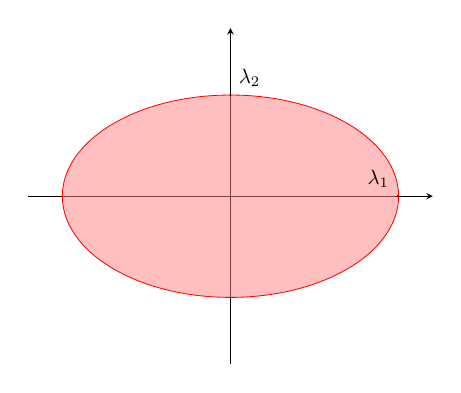
\begin{tikzpicture}[scale=.75]
      \begin{axis}[
        xmin=-2, xmax=2,
        ymin=-2, ymax=2,
        xtick=\empty,
        ytick=\empty,
        axis lines=middle,
        ]
        \draw[red, fill=red!50, fill opacity=0.5] (axis cs:0,0) ellipse [rotate=90, x radius=1, y radius=2];
        \node[label={45:{$\lambda_2$}},circle,fill,inner sep=0pt] at (axis cs:0,1.2) {};
        \node[label={135:{$\lambda_1$}},circle,fill,inner sep=0pt] at (axis cs:1.65,0) {};
      \end{axis}
    \end{tikzpicture}
  \end{minipage}
  \end{example}

  \begin{example}[Vitali 1905]
    $\script{P}(\mathbb{R}^n) \neq \script{M}(\lambda^n)$\\
    Beweis siehe Aufschrieb.
  \end{example}

  
  \chapter{Lebesgue-Integral}
  \begin{definition}
    $X$ Menge, $\mu$ äußeres Maß. Eine funktion $\zeta: X \to \mathbb{R}$ heißt $\bm{\mu}$\textbf{-Treppenfunktion}, wenn sie $\mu$-messbar ist und nur eindlich viele Funktionswerte annimmt.\\
    Die Menge $\script{T}(\mu)$ der $\mu$-Treppenfunktionen ist ein $\mathbb{R}$-Vektorraum. Wir setzen
    \begin{align*}
      \script{T}^+(\mu)=\{\zeta \in \script{T}(\mu) \ | \ \zeta \geq 0\}
    \end{align*}
  \end{definition}

  \begin{example}
    $E \subseteq X, \psi_E: X \to \mathbb{R}, \psi_E(x) = \begin{cases}
      1 & ,x \in E\\
      0 & ,\text{ sonst}
    \end{cases}$  Es ist: $\psi_E$ $\mu$-Treppenfunktion $\Leftrightarrow E \in \script{M}(\mu)$\\
    Sei $\zeta \geq 0, \zeta = \sum\limits_{i=1}^k s_i \psi_{A_i}$ mit $A_i$ messbar und $s_i \geq 0$ und die $A_i$ sind paarweise disjunkt. So eine Darstellung heißt \textbf{einfach}.\\
    Wir setzen:
    \begin{align*}
      (\star) \ I(\zeta) := \sum\limits_{i=1}^k s_i \mu(A_i)
    \end{align*} 
    Für $\zeta=0$ folgt $I(\zeta) = 0 \cdot \mu(X) = 0$\\
    Jedes $\zeta \in \script{T}^+(\mu)$ besitzt eine einfache Darstellung, z.B. können wir für $s_i$ die endlich vielen Funktionswerte wählen und $A_i = \{\zeta = s_i\}$
  \end{example}

  \begin{lemma}
    Das Integral $I: \script{T}^+(\mu) \to [0,\infty]$ ist durch $(\star)$ wohldefiniert. Für $\zeta, \phi \in \script{T}^+(\mu)$ und $\alpha, \beta \in [0, \infty)$ gilt:
    \begin{enumerate}[label=\roman*)]
      \item $I(\alpha \zeta + \beta \psi) = \alpha I(\zeta) + \beta I(\psi)$
      \item $\zeta \leq \psi \implies I(\zeta) \leq I(\psi)$ 
    \end{enumerate}
  \end{lemma}

  \begin{proof}
    Sei $\zeta = \sum\limits_{i=1}^{k} s_i \script{Y_{A_i}}$ einfach $\implies \{\zeta > 0\} = \bigcup\limits_{i;s_i >0} A_i$.\newline
    Schrift extrem unleserlich!!!
  \end{proof}

  \begin{remark}
    Für $A_i$ messbar und $s_i \geq 0$ folgt aus i) auch für $A_i$ nicht disjunk:
    \begin{align*}
      I(\zeta) = \sum\limits_{i=1}^k s_i \mu(A_i) \ \ \text{ für } \zeta = \sum\limits_{i=1}^k s_i \psi_{A_i}
    \end{align*}
  \end{remark}

  \begin{definition}[Lebesgue-Integral]
    Für $f: X \to [0,\infty]$ $\mu$-messbar, setze
    \begin{align*}
      \int f d\mu = sup\{I(\zeta) \ | \ \zeta \in \script{T}^+(\mu), \zeta \leq f\}
    \end{align*}
    $\zeta$ heißt \textbf{Unterfunktion} von f.\\
    Ist $f: X \to [-\infty, \infty]$ $\mu$-messbar und sind die Integrale von $f^{\pm}$ nicht beide unendlich, so setzen wir
    \begin{align*}
      \int f d\mu = \int f^+ d\mu - \int f^- d\mu \ \ \in [-\infty, \infty] 
    \end{align*}
  \end{definition}

  \begin{remark}
    Für $f \geq 0$ sind beide Schritte kompatibel, denn dann gilt $f = f^+$ und $f^- = 0$
  \end{remark}

  \begin{lemma}
    Für $f \in \script{T}^+(\mu)$ gilt: $\int f d\mu = I(f)$
  \end{lemma}

  \begin{proof}
    siehe Aufschrieb
  \end{proof}

  \begin{example}
    $\chi_{\mathbb{Q}}$ ist eine $\lambda^1$-Treppenfunktion und es gilt:\\
    $\int \chi_{\mathbb{Q}} d\lambda^1 = I(\chi_{\mathbb{Q}}) = 0 \cdot \lambda^1(\mathbb{R} \setminus \mathbb{Q}) + 1 \cdot \lambda^1(\mathbb{Q}) = 0 + 1 \cdot 0 = 0$
  \end{example}

  \begin{definition}
    $f:X \to \bar{\mathbb{R}}$ heißt \textbf{integrierbar} bzgl. $\mu$, wenn sie $\mu$-messbar ist und wenn gilt:
    \begin{align*}
      \int f d\mu \in \mathbb{R} \Leftrightarrow \int f^+ d\mu + \int f^- d\mu < \infty
    \end{align*}
  \end{definition}

  \begin{example}
    $\mu = card, X = \mathbb{N}_0$\\
    z.z.: $f: \mathbb{N}_0 \to \mathbb{R}$ ist bzgl. $card$ auf $\mathbb{N}_0$ integrierbar $\implies \sum\limits_{k \in \mathbb{N}} f(k)$ absolut konvergent\\
    Dann gilt: $\int f d card = \sum\limits_{k \in \mathbb{N}} f(k)$\\
    Beweis siehe Aufschrieb
  \end{example}

  \begin{theorem}
    $f,g:X \to \bar{\mathbb{R}}$ $\mu$-messbar. Ist $f \leq g$ $\mu$-fast überall und $\int f^- d\mu < \infty$, so existieren beide Integrale und es ist: $\int f d\mu \leq \int g d\mu$\\
    \glqq$\geq$\grqq gilt entsprechend wenn $f^+ d\mu < \infty$
  \end{theorem}

  \begin{proof}
    siehe Aufschrieb
  \end{proof}

  \begin{remark}
    $f,g: X \to \bar{\mathbb{R}}$, $f$ $\mu$-messbar und $g = f$ $\mu$-fast überall $\stackrel{\text{Kapitel II}}{\implies} g$ $\mu$-messbar\\
    Satz IV.6 $\implies \int g^{\pm} d\mu = \int f^{\pm} d\mu \implies \int f d\mu = \int g \ d\mu$
  \end{remark}

  \sidenote{Vorlesung 12}{11.11.2020}

  \begin{remark}
    Einschub: zum Beweis von Satz III.7
    siehe Aufschrieb
  \end{remark}

  \begin{lemma}[Tschebyscheff-Ungleichung]
    Für $f:X \to [0, \infty]$ $\mu$-messbar mit $\int f d\mu < \infty$ gilt:
    \begin{align*}
      \mu(\{f\geq s\}) \leq \begin{cases}
        \dfrac{1}{s} \cdot \int f d\mu & \text{ für } s \in (0, \infty)\\
        0 & \text{ für } s = \infty
      \end{cases}
    \end{align*}
  \end{lemma}

  \begin{proof}
    siehe Aufschrieb
  \end{proof}

  \begin{lemma}
    Sei $f: X \to \bar{\mathbb{R}}$ $\mu$-messbar.
    \begin{enumerate}[label=\roman*)]
      \item ist $\int f d\mu < \infty \implies \{f = \infty\}$ ist $\mu$-Nulllmenge
      \item ist $f \geq 0$ und $\int f d\mu = 0 \implies \{f > 0\}$ ist $\mu$-Nullmenge
    \end{enumerate}
  \end{lemma}

  \begin{proof}
    siehe Aufschrieb
  \end{proof}

  \begin{theorem}
    Zu $f: X \to [0,\infty]$ $\mu$-messbar gibt es eine Folge $f_k \in \script{T}^+(\mu)$ mit $f_0 \leq f_1 \leq ...$ und $\lim\limits_{k \to \infty} f_k(x) = f(x) \ \forall x \in X$.
  \end{theorem}

  \begin{proof}
    siehe Aufschrieb
  \end{proof}

  \newpage
  \begin{theorem}[Monotonie Konvergenz / Beppo-Levi]
    Seien $f_k:X \to [0,\infty]$ $\mu$-messbar mit $f_1 \leq f_2 \leq ...$ und $f: X \to [0, \infty]$ mit $f(x) := \lim\limits_{k \to \infty} f_k(x)$. Dann gilt:
    \begin{align*}
      \int f d\mu = \lim\limits_{k \to \infty} \int f_k \ d\mu
    \end{align*}
  \end{theorem}

  \begin{proof}
    siehe Aufschrieb
  \end{proof}

  \begin{theorem}
    $f,g: X \to \bar{\mathbb{R}}$ integrierbar bzgl. $\mu$, so ist auch $\alpha f + \beta g$ integrierbar $\forall \alpha, \beta \in \mathbb{R}$ und es gilt:
    \begin{align*}
      \int (\alpha f + \beta g) \ d\mu = \alpha \int f d\mu + \beta \int g d\mu
    \end{align*}
  \end{theorem}

  \begin{proof}
    siehe Aufschrieb
  \end{proof}

  \begin{definition}
    Sei $\mu$ ein äußeres Maß auf $X$ und $E \subseteq X$ sei $\mu$-messbar. Dann setzen wir, falls das rechte Integral existiert
    \begin{align*}
      \int\limits_E f d\mu = \int f \chi_E d\mu
    \end{align*}
    $f$ heißt \textbf{auf $\bm{E}$ integrierbar}, wenn $f \chi_E$ integrierbar ist.
  \end{definition}

  \begin{remark}
    Wegen $(f \chi_E)^{\pm} = f^{\pm} \chi_E \leq f^{\pm}$ existiert das Integral von $f$ über $E$ auf jeden Fall dann, wenn $\in f d\mu$ existiert. (Speziell für $f \geq 0$)
  \end{remark}

  \begin{example}
    $\alpha \in \mathbb{R}, \ f:\mathbb{R}^n \to \mathbb{R}, \ f(x) = ||x||^{-\alpha}$\\
    Beh: 
    \begin{align*}
      \int\limits_{\mathbb{R}^n \setminus B_1(0)} f d\lambda^n < \infty &\Leftrightarrow \alpha > n\\
      \int\limits_{B_1(0)} f d\lambda^n < \infty &\Leftrightarrow \alpha < n
    \end{align*}
    Beweis siehe Aufschrieb
  \end{example}

  \newpage
  \sidenote{Vorlesung 13}{14.12.20}
  \begin{theorem}
    Sei $f: X \to \bar{\mathbb{R}}$ $\mu$-messbar. Dann gelten:
    \begin{enumerate}[label=\roman*)]
      \item $f$ integrierbar $\Leftrightarrow |f|$ integrierbar
      \item Es gilt: $|\int f d\mu| \leq \int |f| d\mu$, falls das Integral von $f$ existiert
      \item Ist $g: X \to [0, \infty]$ $\mu$-messbar mit $|f| \leq g$ $\mu$-fast überall und $\int g d\mu < \infty$, so ist $f$ integrierbar 
    \end{enumerate}
  \end{theorem}

  \begin{proof}
    siehe Aufschrieb
  \end{proof}

  \begin{example}
    $f: \mathbb{R}^n \to \bar{\mathbb{R}}$ $\lambda^n$-messbar und es gelte für ein $C \in [0, \infty]$:\\
    $|f(x)| \leq C ||x||^{-\alpha}$ fast überall in $B_{\epsilon}(0)$ mit $(\alpha < n)$ bzw.\\
    $|f(x)| \leq C ||x||^{-\alpha}$ fast überall in $\mathbb{R}^n \setminus B_{\epsilon}(0)$ mit $\alpha > n$\\
    $\implies f$ ist auf $B_{\epsilon}(0)$ bzw. $\mathbb{R}^n \setminus B_{\epsilon}(0)$ integrierbar
  \end{example}

  
  \chapter{Konvergenzsätze und $L^n$-Räume}
  \begin{example}
    Punktweise Konvergenz reicht nicht für Konvergenz der Integrale.\\
    Für $\epsilon > 0$ sei $f_{\epsilon}: \mathbb{R} \to \mathbb{R}, f_{\epsilon} = \dfrac{1}{2\epsilon} \chi_{[-\epsilon, \epsilon]}$\\
    Es gilt $f_{\epsilon}(x) = 0$ für $\epsilon < |x|$\\
    $\implies f(x) := \lim\limits_{\epsilon \downarrow 0} f_{\epsilon}(x) = \begin{cases}
      0 & \text{, für } x \neq 0\\
      \infty & \text{, für } x = 0
    \end{cases}$\\
    Weiter $\int f_{\epsilon} d\lambda^1 = \dfrac{1}{2\epsilon} \lambda^1([-\epsilon, \epsilon]) = 1 \ \forall \epsilon > 0$\\
    $\implies \int f d\lambda^1 = 0 < 1 = \lim\limits_{\epsilon \downarrow 0} f_{\epsilon} d\lambda^1$
  \end{example}

  \begin{theorem}[Lemma von Fatou]
    $f_k: X \to [0,\infty]$ Folge von $\mu$-messbaren Funktionen.\\
    Für $f: X \to \bar{\mathbb{R}}, f(x) = \liminf\limits_{k \to \infty} f_k(x)$ gilt:
    \begin{align*}
      \int f d\mu \leq \liminf\limits_{k \to \infty} \int f_k d\mu
    \end{align*}
  \end{theorem}

  \begin{proof}
    siehe Aufschrieb
  \end{proof}

  \begin{theorem}[Dominierte Konvergenz bzw. Satz von Lebesgue]
    $f_1, f_2, ...$ Folge von $\mu$-messbare Funktionen und $f(x) = \lim\limits_{k \to \infty} f_k(x)$ für $\mu$-fast alle $x \in X$. Es gebe eine integrierbare Funktion $g: X \to [0, \infty]$ mit $\sup\limits_{k \in \mathbb{N}} |f_k(x)| \leq g(x)$ für $\mu$-fast alle $x$. Fann ist $f$ integrierbar und $\int f d\mu = \lim\limits_{k \to \infty} \int f_k d\mu$.\\
    Es gilt sogar $||f_k \cdot f||_{L^1(y)} := \int |f_k -f| d\mu \to 0$
  \end{theorem}

  \begin{proof}
    siehe Aufschrieb
  \end{proof}

  \begin{remark}[Anwendung]
    Vergleich Riemann-$\int$ mit Lebesgue-$\int$\\
    Sei $I=[a,b]$ kompaktes Intervall, $f:I \to \mathbb{R}$ beschränkt. Unterteilungspunkte $a = x_0 \leq ... \leq x_N = b$ $\to$ Zerlegung $Z$ von $I$ mit Teilintervallen $I_j = [x_{j-1}, x_j]$\\
    $\bar{S}_Z(f) = \sum\limits_{j=1}^N (\sup\limits_{I_j} f) (x_j - x_{j-1}), \ \ \ \underbar{S}_Z(f)= \sum\limits_{j=1}^N (\inf\limits_{I_j} f)(x_j-x_{j-1})$\\
    Für Zerlegungen $Z_1, Z_2$ mit Verfeinerung $Z_1 \cup Z_2$\\
    $\implies \underbar{S}_{Z_1}(f) \leq \underbar{S}_{Z_1 \cup Z_2}(f) \leq \bar{S}_{Z_1 \cup Z_2}(f) \leq \bar{S}_{Z_2}(f)$\\
    $f$ heißt \textbf{Riemann-integrierbar} mit Integral $\int\limits_a^b f(x) dx = S$, falls gilt:\\
    $\sup\limits_Z \underbar{S}_Z(f) = \inf\limits_Z \bar{S}_Z(f) = S$
  \end{remark}

  \begin{theorem}
    $f: I \to \mathbb{R}$ beschränkt auf kompaktem Intervall $I=[a,b]$. Dann gilt:\\
    $f$ Riemann-integrierbar $\Leftrightarrow \lambda^1(\{x \in I \ | \ f \text{ ist nicht stetig in } x\}) = 0$\\
    In diesem Fall ist $f$ auch Lebesgue-integrierbar und die Integrale stimmen überein.
  \end{theorem}

  \begin{proof}
    siehe Aufschrieb
  \end{proof}

  \begin{theorem}
    $X$ metrischer Raum, $\mu$ Maß auf $Y$ und $f:X \times Y \to \mathbb{R}$ mit $f(x, \cdot)$ integrierbar bzgl. $\mu \ \forall x \in X$.\\
    Betrachte $F: X \to \mathbb{R}, F(x) = \int f(x,y) d\mu(y)$\\
    Sei $f(\cdot, y)$ stetig in $x_0 \in X$ für $\mu$-fast alle $y \in Y$. Weiter gebe es eine $\mu$-integrierbare Funktion $g: Y \to [0, \infty]$, so dass für alle $x \in X$ gilt: $|f(x,y)| \leq g(y) \ \forall y \in Y \setminus N_X$ mit einer $\mu$-Nullmenge $N_x$.\\
    Dann ist $F$ stetig in $x_0$.
  \end{theorem}

  \begin{proof}
    siehe Aufschrieb
  \end{proof}

   \sidenote{Vorlesung 14}{18.12.20}

  \begin{theorem}
    Sei $I \subseteq \mathbb{R}$ offenes Intervall, $\mu$ Maß auf $Y$ und $f: I \times Y \to \mathbb{R}$ mit $f(x, \cdot)$ integrierbar bzgl. $\mu$ für alle $x \in I$.\\
    Setze $F: U \to \mathbb{R}, F(x) = \int f(x,y) d\mu(y)$\\
    Es sei $f(\cdot, y)$ in $x_0$ differenzierbar für $\mu$-fast alle $y \in Y$ und es existiere $g: Y \to [0, \infty]$ $\mu$-integrierbar mit
    \begin{align*}
      \dfrac{|f(x,y) - f(x_0, y)|}{|x-x_0|} \leq g(y) \ \forall x\in I \ \forall y \in Y \setminus N_x
    \end{align*} 
    mit einer $\mu$-Nullmenge $N_x$. Dann folgt:
    \begin{align*}
      F'(x_0) = \int \dfrac{\partial f}{\partial x} (x_0, y) d\mu(y)
    \end{align*}
  \end{theorem}
  \begin{proof}
    siehe Aufschrieb
  \end{proof}

  \newpage

  \begin{lemma}
    $\script{U} \subseteq \mathbb{R}^n$ offen, $\mu$ Maß auf $Y$ und $f: \script{U} \times Y \to \mathbb{R}$ mit $f$ integrierbar bzgl. $\mu \ \forall x \in \script{U}$. Betrachte $F: \script{U} \to \mathbb{R}, F(x) = \int f(x,y) d\mu(y)$\\
    Es gebe eine $\mu$-Nullmenge $N \subseteq Y$, so dass $\forall y \in Y \setminus N$ gilt:
    \begin{align*}
      f(\cdot, y) \in C^1(\script{U}) \text{ und } |D_x f(x,y)| \leq g(y) \text{ mit } g: Y \to [0, \infty] \text{ integrierbar}
    \end{align*}
    $\implies F \in C^1(\script{U})$ und $\forall x \in \script{U}$ gilt:
    \begin{align*}
      \dfrac{\partial F}{\partial x_i}(x) = \int \dfrac{\partial f}{\partial x_i}(x,y) d\mu(y)
    \end{align*}
  \end{lemma}

  \begin{proof}
    siehe Aufschrieb
  \end{proof}

  \begin{example}
    \begin{align*}
      \int\limits_0^{\infty} \dfrac{\sin(x)}{x} dx = ? \ \ \ \ \text{Betrachte $F: [0, \infty] \to \mathbb{R}, F(t) = \int\limits_0^{\infty} e^{-tx} \dfrac{\sin{x}}{x} dx$}
    \end{align*}
    $f(t,x) := e^{-tx} \dfrac{\sin(x)}{x}$ hat für $t \geq \delta$ die Abschätzungen\\
    $|f(t,x)|, |\partial_t f(t,x)| \leq e^{-\delta x} =: g(x) \in L^1([0, \infty))$\\
    Lemma V.6 $\implies \forall t > 0$ gilt: 
    \begin{align*}
      F'(t) &= \int\limits_0^{\infty} e^{-tx} (-\sin{x}) dx\\
            &= [e^{-tx} \cos{x}]_{x=0}^{x=\infty} + t \int\limits_0^{\infty} e^{-tx} \cos{x} dx\\
            &= -1 + t^2 \int\limits_0^{\infty} e^{-tx} \sin{x} dx\\
            &= -1 - t^2 F'(t)
    \end{align*}
    $\implies F'(t) = \dfrac{-1}{1+t^2}$\\
    \newline
    ... (siehe Aufschrieb)\\
    \newline
    $\int\limits_0^{\infty} \dfrac{\sin(x)}{x} dx = \dfrac{\pi}{2}$
  \end{example}

  \newpage
  \begin{definition}[$L^p$-Norm]
    Für $\mu$-messbares $f: X \to \bar{\mathbb{R}}$ und $1 \leq p \leq \infty$ setzen wir
    \begin{align*}
      ||f||_{L^p(\mu)} := \begin{cases}
        (\int |f|^p d\mu)^{1/p} & \text{, für } 1\leq p < \infty\\
        \inf\{s>0 \ | \ \mu(\{|f| > s\})=0\} & \text{, für } p = \infty
      \end{cases}
    \end{align*}
    auf $\script{L}^p(\mu) = \{f:X \to \bar{\mathbb{R}} \ | \ f \mu-\text{messbar }, ||f||_{L^p(\mu)} < \infty\}$\\
    Betrachte Äquivalenzrelation $f\sim g \Leftrightarrow f(x) = g(x)$ für $\mu$-fast alle $x \in X$, und definiere den $\bm{L^p}$\textbf{-Raum} durch $\script{L}^p(\mu)/_{\sim}$.
  \end{definition}

  \begin{definition}
    Für $E \subseteq X$ messbar und $f: E \to \bar{\mathbb{R}}$ sei $f_0: X\to \bar{\mathbb{R}}$ die \textbf{Fortsetzung} mit $f_0(x)=0 \ \forall x \in X \setminus E$. Wir setzen dann
    \begin{align*}
      \script{L}^p(E) := \{f:E \to \bar{\mathbb{R}} \ | \ f_0 \in \script{L}^p(\mu)\}
    \end{align*}
    und $L^p(E,\mu) := \script{L}^p(E)/_{\sim}$.
  \end{definition}

  \begin{proposition}
    Für $1 \leq p \leq \infty$ ist $(L^p(\mu), ||\cdot||_{L^p(\mu)})$ ein normierter Vektorraum. Insbesondere gelten für $\lambda \in \mathbb{R}$ und $f,g \in L^p(\mu)$:
    \begin{enumerate}
      \item $||f||_{L^p} = 0 \implies f = 0$ $\mu$-fast überall
      \item $f \in L^p(\mu), \lambda \in \mathbb{R} \implies \lambda f \in L^p(\mu), \ ||\lambda f||_{L^p} = |\lambda| \ ||f||_{L^p}$
      \item $f,g \in L^p(\mu) \implies f+g \in L^p(\mu)$ und $||f+g||_{L^p} \leq ||f||_{L^p} + ||g||_{L^p}$
    \end{enumerate}
  \end{proposition}

  \begin{proof}
    siehe Aufschrieb
  \end{proof}

  \begin{lemma}[Youngsche Ungleichung]
    Für $1 < p,q < \infty$ mit $\dfrac{1}{p} + \dfrac{1}{q} = 1$ und $x,y \geq 0$ gilt: \ \ $xy \leq \dfrac{x^p}{p} + \dfrac{y^q}{q}$
  \end{lemma}

  \begin{proof}
    siehe Aufschrieb
  \end{proof}

  \newpage
  \begin{theorem}[Höldersche Ungleichung]
    Für $\mu$-messbare $f,g: X \to \bar{\mathbb{R}}$ gilt: \ \ $|\int fg d\mu| \leq ||f||_{L^p} ||g||_{L^p}$,\\
    falls $1 \leq p,q \leq \infty$ mit $\dfrac{1}{p} + \dfrac{1}{q} = 1$
  \end{theorem}

  \begin{proof}
    siehe Aufschrieb
  \end{proof}

  \begin{theorem}[Minkowski-Ungleichung]
    Für $f,g \in L^p(\mu)$ mit $1 \leq p \leq \infty$ gilt: \ \ $|| f+g ||_{L^p} \leq ||f||_{L^p} + ||g||_{L^p}$
  \end{theorem}

  \begin{proof}
    siehe Aufschrieb
  \end{proof}

  \begin{lemma}
    Sei $1 \leq p < \infty$ und $f_k = \sum\limits_{j=1}^k u_j$ mit $u_j \in L^p(\mu)$. Falls $\sum\limits_{j=1}^k ||u_j||_{L^p} < \infty$, so gelten:
    \begin{enumerate}[label=\roman*)]
      \item $\exists \ \mu$-Nullmenge $N$: $f(x) = \lim\limits_{k \to \infty} f_k(x) \ \forall x \in X \setminus N$ ex.
      \item mit $f := 0$ auf gilt $f \in L^p(\mu)$
      \item $||f - f_k||_{L^p} \to 0$ mit $k \to \infty$
    \end{enumerate}
  \end{lemma}

  \begin{proof}
    siehe Aufschrieb
  \end{proof}

  \begin{theorem}[Satz von Riesz-Fischer]
    $(L^p(\mu), ||\cdot||_{L^p})$ ist vollständig, also ein Banachraum. $(1 \leq p \leq \infty)$
  \end{theorem}
  \begin{proof}
    siehe Aufschrieb
  \end{proof}

  \begin{lemma}
    Konvergiert $f_k$ gegen $f$ in $L^p(\mu)$, so konvergiert eine Teilfolge $f_{k_j}$ punktweise $\mu$-fast überall gegen $f$.
  \end{lemma}  
  
  \begin{example}
    Im Fall $p < \infty$ kann im Allgemeinen nicht auf die Wahl einer Teilfolge verzichtet werden:\\
    Jedes $n \in \mathbb{N}$ besitzt die eindeutige Darstellung $n=2^k+j$ mit $k \in \mathbb{N}_0, 0 \leq j < 2^k$\\
    Definiere damit $f_n:[0,1] \to \mathbb{R}, f_n(x) = \begin{cases}
      1 & \text{, falls } j \cdot 2^{-k} \leq x \leq (j+1) 2^{-k}\\
      0 & \text{, sonst}
    \end{cases}$\\
    $\int\limits_0^1 f_n(x) dx = 2^{-k} < \dfrac{2}{n} \to 0$ mit $n \to \infty$\\
    Andererseits: $\limsup\limits_{n \to \infty} f_n(x) = 1 \ \forall x \in [0,1)$, denn zu $x \in [0,1), k \in \mathbb{N}$ können wir\\
    $j \in \{0,1,...,2^k-1\}$ wählen mit $j \cdot 2^{-k} \leq x < (j+1) 2^{-k}$\\
    $\implies f_n(x) = 1$ für $n = 2^k+j$\\
    $\implies$ Folge konvergiert nicht punktweise $\lambda^1$-fast überall gegen $0$.
  \end{example}

  \begin{remark}
    Jetzt betrachten wir $\mu=\lambda^n$ im $\mathbb{R}^n$.\\
    Im $\mathbb{R}^n$ haben wir eine Metrik.
  \end{remark}

  \begin{definition}
    Der \textbf{Träger} einer Funktion $f:\Omega \to \mathbb{R}, \Omega \subseteq \mathbb{R}^n$ offen, ist die Menge 
    \begin{align*}
      spt(f) = \overline{\{x \in \mathbb{R} \ | \ f(x) \neq 0\}}
    \end{align*}
    Der Raum der stetigen Funktionen mit kompaktem Träger in $\Omega$ wird mit $C_c^0(\Omega)$ bezeichnet.\\
    Für $K \subseteq \Omega$ kompakt sei $dist(\cdot, K): \mathbb{R}^n \to [0, \infty), dist(x, K) = \inf\limits_{z \in K} ||x - z||$ die \textbf{Abstandsfunktion} von K.\\
    Wir benötigen:
    \begin{enumerate}
      \item $dist(\cdot, K)$ ist Lipschitz-stetig mit Konstante $1$
      \item $dist(\mathbb{R}^n \setminus \Omega, K) = \inf\limits_{x \in \mathbb{R}^n \setminus \Omega} dist(x, K) > 0$
    \end{enumerate}
  \end{definition}

  \begin{theorem}
    Sei $\Omega \subseteq \mathbb{R}^n$ offen und $1 \leq p < \infty$. Dann existiert zu jedem $f \in C^p(\Omega)$ eine Folge $f_k \in C_c^0(\Omega)$ mit $|| f_k - f||_{L^p(\Omega)} \to 0$ mit $k \to \infty$.
  \end{theorem}
  \begin{proof}
    siehe Aufschrieb
  \end{proof}

  \begin{remark}
    $BC^0(\Omega)$ bezeichnet die Menge der beschränkten, stetigen Funktionen auf $\Omega$. Mit Supremumsnorm $||\cdot||_{sup}$ ist diese ein Banachraum.\\
    ... (Rest siehe Aufschrieb)
  \end{remark}

  \begin{theorem}
    Für $f \in L^2(I, \mathbb{C})$ konvergiert $f_n$ gegen $f$ in $L^2(I, \mathbb{C})$? (bezieht sich auf Bem. vorher)
  \end{theorem}
  \begin{proof}
    siehe Aufschrieb
  \end{proof}

  \begin{remark}
    Sei $\ell^2(\mathbb{C})$ der Raum aller komplexen Folgen $c = (c_k)_{k \in \mathbb{Z}}$ mit $||c||_{\ell^2}^2 = 2 \pi \sum\limits_{k \in \mathbb{Z}} |c_k|^2 < \infty$\\
    $\ell^2(\mathbb{C})$ ist vollständig (folgt aus Riesz-Fischer angewandt auf das Zählmaß auf $\mathbb{Z}$)
  \end{remark}

  \newpage
  \begin{lemma}
    Die Abbildung $\script{F}: (L^2(I, \mathbb{C}), ||\cdot||_{L^2}) \to (\ell^2(\mathbb{C}), ||\cdot||_{\ell^2}), \script{F}(f) = (\hat{f}(k))_{k \in \mathbb{Z}}$ ist eine Isometrie von Hilberträumen.
  \end{lemma}
  \begin{proof}
    siehe Aufschrieb
  \end{proof}

  \begin{remark}
    Die Konvergenz der Fourierreihe ist ein Spezialfall des Spektralsatzes für selbstadjungierte Operatoren. Dieser verallgemeinert die Diagonalisierbarkeit symmetrischer Matrizen (siehe LA) auf $\infty$-dimensionalen Räume.\\
    Hier ist der Operator $H = -\dfrac{d^2}{dx^2}$ ein Endomorphismus auf $C_{Per}^{\infty}(I)$\\
    $H:C_{Per}^{\infty}(I) \to C_{Per}^{\infty}(I), Hf=-\dfrac{d^2f}{dx^2}$\\
    Part. Int. $\implies \langle Hf,g \rangle_{L^2} = \langle f,Hg \rangle_{L^2} \ \forall f,g \in C_{Per}^{\infty}(I)$ sowie $\langle Hf, f \rangle_{L^2} = ||\dfrac{df}{dx}||_{L^2}^2 \geq 0$\\
    Die $w_k$ sind Eigenfunktionen von den Eigenvektoren $\lambda_k = k^2$:\\
    $Hw_k = \lambda^2 w_k \ \forall k \in \mathbb{Z}$\\
    Satz V.18: Der von den Eigenfunktionen $w_k$ aufgespannte Raum ist dicht in $L^2(I, \mathbb{C})$
  \end{remark}
  \chapter{Satz von Fubini}
  \begin{remark}[Prinzip von Cavalieri]
    Haben zwei Körper in jeder Höhe Schnitte von gleichem Flächeninhalt, so haben sie auch auch das gleiche Volumen.    
  \end{remark}

  \begin{example}
    \begin{enumerate}
      \item Volumen eines Kegels.\\
        Sei $B \subseteq \mathbb{R}^2$ ein Gebiet mit Flächeninhalt $|B| = A$.\\
        Betrachte $C = \{s(b,1) \ | \ b \in B, 0 \leq s \leq 1\}$\\
        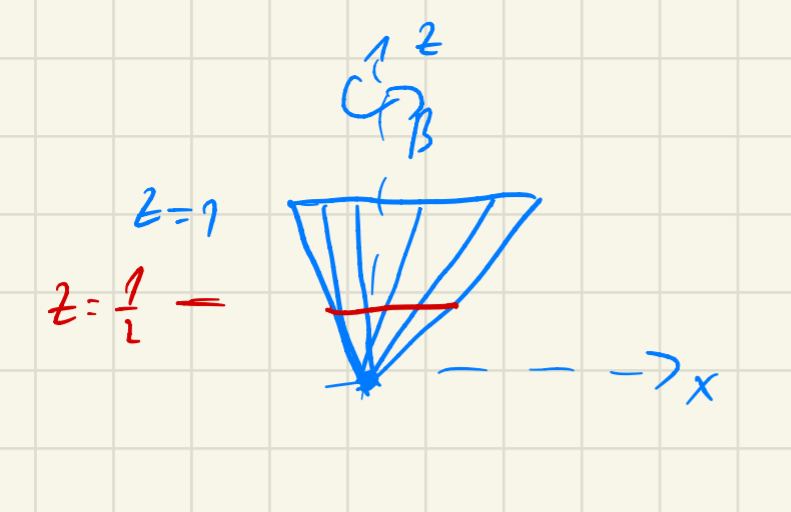
\includegraphics[width=3.5cm]{img/VI_Bsp_1_Kegel.png}\\
        Für $k \in [0,1]$ ist der $k$-Schnitt von $C$ die Menge \\
        $C_k = \{a \in \mathbb{R}^2 \ | \ (a,b) \in C\} = \{h \cdot b \ | \ b \in B\} = kB$\\
        $|C_k| = k^2A$ Nach Cavalieri hängt $vol(C)$ nur von $A$ ab.\\
        Wir schreiben $vol(C) = V(A)$. Es gilt $V(kA) = kV(A)$ für $k \in \mathbb{N}$, betrachte dazu ... (siehe Aufschrieb)
        \item Betrachte in $\mathbb{R}^3 = \mathbb{R}^2 \times \mathbb{R}$ die Mengen und die Inhalte der Zugehörigen $z$-Schnitte:
        \begin{align*}
          &\text{Zylinder } Z=\{(x,y,z) \ | \ \sqrt{x^2 + y^2} \leq 1, 0 \leq z \leq 1\}, |Z_z| = \pi\\
          &\text{Kegel } C=\{(x,y,z) \ | \ \sqrt{x^2 + y^2} \leq z, 0 \leq z \leq 1\}, |C_z| = \pi z^2\\
          &\text{Halbkugel } H=\{(x,y,z) \ | \ \sqrt{x^2 + y^2} \leq \sqrt{1-z^2}, 0 \leq z \leq 1\}, |H_z| = \pi (1-z^2)\\
        \end{align*}
        $\implies |Z_z| = |C_z| + |H_z| \stackrel{Cavalieri}{\implies} vol(H) = vol(Z) - vol(C) = \pi - \frac{\pi}{3} = \frac{2}{3} \pi$\\
        $\implies vol(C) : vol(H) : vol(Z) = 1 : 2 : 3$ (Archimedes)
    \end{enumerate}
  \end{example}

  \begin{definition}
    Seien $\alpha, \beta$ äußere Maße auf $X,Y$. Das \textbf{Produktmaß} $\alpha \times \beta$ einer Menge $E \subseteq X \times Y$ ist
    \begin{align*}
      (\star) \ \ \alpha \times \beta (E) = inf\{\sum\limits_{j=1}^{\infty} \alpha(A_j) \beta(B_j) \ | \ A_j, B_j \text{ messbar}, E \subseteq \bigcup\limits_{j=1}^{\infty} A_j \times B_j\}
    \end{align*}
  \end{definition}

  \begin{lemma}
    $\alpha \times \beta$ ist ein äußeres Maß
  \end{lemma}
  \begin{proof}
    siehe Aufschrieb
  \end{proof}

  \begin{lemma}
    Sei $P = A \times B$. Eine Produktmenge, d.h. $A,B$ sind messbar bzgl. $\alpha$ bzw. $\beta$. Dann gilt $\alpha \times \beta(P) = \alpha(A) \beta(B)$ und $P$ ist $\alpha \times \beta$-messbar.
  \end{lemma}
  \begin{proof}
    siehe Aufschrieb
  \end{proof}

  \begin{theorem}[Cavalierisches Prinzip]
    Seien $\alpha$ und $\beta$ $\sigma$-endliche äußere Maße auf $X$ bzw. $Y$, und $D \subseteq X \times Y$ sei $\alpha \times \beta$-messbar. Dann ist $D_y = \{x \in X \ | \ (x,y) \in D\}$ $\alpha$-messbar für $\beta$-fast alle $y \in Y$. Die Funktion $y \mapsto \alpha(D_y)$ ist $\beta$-messbar und es gilt:
    \begin{align*}
      (\alpha \times \beta)(D) = \int\limits_Y \alpha(D_y) \ d\beta(y)
    \end{align*}
  \end{theorem}
  \sidenote{Vorlesung 17}{11.01.21}
  \begin{proof}
    siehe Aufschrieb
  \end{proof}

  \begin{remark}
    Die Rollen von $\alpha$ und $\beta$ können vertauscht werden, d.h. man betrachtet das $\beta$-Maß des $X$-Schnittes $D_x 0 \{y \in Y \ | \ (x,y) \in D\}$ und integriert bzgl. $\alpha$
    \begin{align*}
      \implies \alpha \times \beta (D) = \int\limits_Y \alpha(D_y) \ d\beta(y) = \int\limits_X \beta(D_x) \ d\alpha(x)
    \end{align*}
  \end{remark}

  \begin{example}
    Man kann nicht auf die $\sigma$-Endlichkeit verzichten.
    \begin{align*}
      D := \{(x,y) \in [0,1] \times [0,1] \ | \ x=y\} \subseteq \mathbb{R} \times [0,1]\\
      \int\limits_{\mathbb{R}} card(D_x) d\lambda^1(x) = 1 \neq 0 = \int\limits_{[0,1]} \lambda^1(D_y) \ d card(y)
    \end{align*}
    Mit $I_k = [\frac{k-1}{n}, \frac{k}{n}]$ gilt $D = \bigcap\limits_{n=1}^{\infty}( \bigcup\limits_{k=1}^{\infty} I_k \times I_k) \implies D$ ist messbar bzgl. $\lambda^1 \times card$
  \end{example}

  \newpage
  \begin{lemma}
    Es gilt $\lambda^n = \lambda^k \times \lambda^m$ für $k + m = n$
  \end{lemma}
  \begin{proof}
    siehe Aufschrieb
  \end{proof}

  \sidenote{Vorlesung 18}{15.01.21}
  \begin{example}
    \begin{enumerate}
      \item[]
      \item Volumen $\alpha_n$ der Kugel $B=\{z \in \mathbb{R}^n \ | \ ||z|| < 1\}.$\\
        Für $y \in [-1,1)$ ist $B_y = \{x \in \mathbb{R}^{n-1} \ | \ ||x|| < |1-y^2|^{1/2}\}$\\
        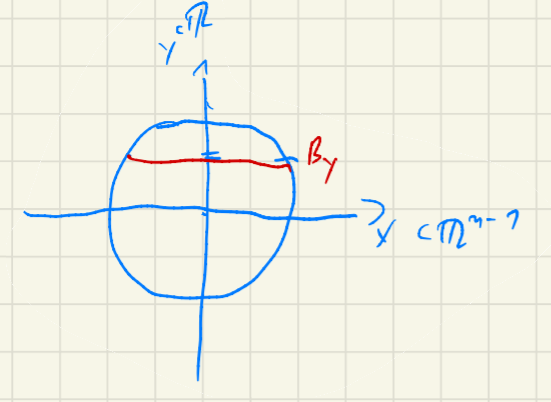
\includegraphics[width=3.5cm]{img/VI_Bsp_3_Kreis.png}
        \begin{align*}
          \alpha_n &=  \int\limits_{-1}^1 \lambda^{n-1}(B_y) \ dy = \alpha_{n-1} \int\limits_{-1}^1 (1-y^2)^{\frac{n-1}{n}} \ dy\\
          &\stackrel{y=\cos \theta}{=} \alpha_{n-1} A_n \text{, mit } A_n = \int\limits_0^{\pi} \sin^n\theta \ d\theta\\
          &\stackrel{part. Int.}{\implies} A_n = \frac{n-1}{n} A_{n-2} \ \forall \ n \geq 2 \text{, dabei sind } A_0 = \pi, A_1 = 2\\
          \implies A_{2k} &= \frac{2k-1}{2k} \cdot ... \cdot \frac{1}{2} A_0 = \pi \prod\limits_{j=1}^k \frac{2j}{2j+1}\\
          A_{2k+1} &= \frac{2k}{2k+1} \cdot ... \cdot \frac{2}{3} A_1 =2 \prod\limits_{j=1}^k \frac{2j}{2j+1}\\
          \implies A_{2k+1} A_{2k} &= \frac{2\pi}{2k+1} \text{ bzw. } A_{2k} A_{2k-1} = \frac{\pi}{k}\\
          \implies \alpha_{2k} &= (A_{2k}A_{2k-1}) ... (A_3 A_2) \alpha_0 = \frac{\pi^k}{k!}\\
          \alpha_{2k+1} &= (A_{2k}A_{2k-1}) ... (A_3 A_2) \alpha_1 = \frac{\pi^k}{(k+\frac{1}{2})(k-\frac{1}{2})...\frac{1}{2}}
        \end{align*}
        Bem: $\alpha_k \to 0$ mit $k \to \infty$
      \item Für $A \subseteq \mathbb{R}^n$ sei $K(A) = \{y (x,1) \in \mathbb{R}^n \times \mathbb{R} = \mathbb{R}^{n-1} \ | \ 0<y<1, x\in A\}$\\
        Beh: $A$ messbar bzgl. $\lambda^n$ $\implies$ $K(A)$ $\lambda^{n+1}$-messbar und $\lambda^{n+1}(K(A)) = \frac{1}{n+1}\lambda^n(A)$\\
        (siehe Aufschrieb)
    \end{enumerate}
  \end{example}

  \begin{definition}
    Eine Funktion $f: X \to [-\infty, \infty]$ heißt $\bm{\sigma}$\textbf{-endlich} bzgl. des äußeren Maßes $\mu$, falls gilt:
    $$f \text{ ist } \mu \text{-messbar und } \{f \neq 0\} \text{ ist } \sigma \text{-endlich}$$
  \end{definition}

  \begin{theorem}[Fubini]
    Seien $\alpha, \beta$ äußere Maße auf $X$ bzw. $Y$ und $f: X \times Y \to \bar{\mathbb{R}}$ sei $\sigma$-endlich bzgl. $\alpha \times \beta$. Ist das Integral $\int f \ d(\alpha \times \beta)$ definiert, so gilt:
    \begin{enumerate}
      \item Für $\beta$-fast alle $y \in Y$ ist $f(\cdot, y) \alpha$-messbar, und $\int\limits_X f(x,y) \ d \alpha(x)$ existiert.
      \item $y \mapsto \int\limits_X f(x,y) \ d\alpha(x)$ ist $\beta$-messbar und $\int\limits_Y \int\limits_X f(x,y) \ d\alpha(x) \ d\beta(y)$ existiert.
      \item $\int\limits_{X\times Y} f \ d(\alpha \times \beta) = \int\limits_Y \int\limits_X f(x,y) \ d\alpha(x) \ d\beta(y)$
    \end{enumerate}
    Der Satz gilt auch mit vertauschten Reihenfolgen der Integrationen, also folgt:
    \begin{align*}
      \int\limits_{X\times Y} f \ d(\alpha \times \beta) = \int\limits_Y \int\limits_X f(x,y) \ d\alpha(x) \ d\beta(y) = \int\limits_X \int\limits_Y f(x,y) \ d\beta(y) \ d\alpha(x)
    \end{align*}
    Zusatz: Ist $f: X \times Y \to \bar{\mathbb{R}} \ \sigma$-endlich und $\int\limits_Y \int\limits_X |f(x,y)| \ d\alpha(x) \ d\beta(y) < \infty$, so ist $f$ integrierbar bzgl. $\alpha \times \beta$ und der Satz damit anwendbar.
  \end{theorem}

  \begin{proof}
    siehe Aufschrieb
  \end{proof}

  \begin{example}
    \begin{enumerate}
      \item[]
      \item 
          $\begin{rcases}
            \int\limits_{-1}^1 \int\limits_{-1}^1 \frac{x^2-y^2}{(x^2+y^2)^2} \ dy \ dx = \pi\\
            \int\limits_{-1}^1 \int\limits_{-1}^1 \frac{x^2-y^2}{(x^2+y^2)^2} \ dx \ dy = -\pi
          \end{rcases} \text{ denn } \frac{x^2-y^2}{(x^2+y^2)^2} = \frac{\partial}{\partial x} \frac{\partial}{\partial y} \arctan(\frac{x}{y}) \text{ für } y \neq 0$\\
          Fubini $\implies$ Integral bzgl. $\lambda^2 = \lambda^1 \times \lambda^1$ ex nicht!
      \item
        \begin{align*}
          \int\limits_{-1}^1 \int\limits_{-1}^1 \frac{xy}{(x^2+y^2)^2} \ dx \ dy = 0 = \int\limits_{-1}^1 \int\limits_{-1}^1 \frac{xy}{(x^2+y^2)^2} \ dy \ dx
        \end{align*}
        Aber das $\lambda^2$-Integral über $[-1,1)^2$ ex. nicht, da
        \begin{align*}
          \int\limits_{[0,1)^2} \frac{xy}{(x^2+y^2)^2} \ d\lambda^2(x,y) = \int\limits_0^1 \int\limits_0^1 \frac{xy}{(x^2+y^2)^2} \ dx \ dy = \frac{1}{2} \int\limits_0^1 (\frac{1}{y} - \frac{y}{1+y^2}) \ dy = \infty
        \end{align*}
    \end{enumerate}
  \end{example}

  \begin{example}
    $\mu$ äußeres Maß auf $X$ und $f: X \to [0, \infty]$ sei $\sigma$-endlich bzgl. $\mu$. Ist $\script{C}:[0,\infty] \to [0, \infty]$ stetig mit $\script{C}(0) = 0$, sowie auf $(0, \infty)$ stetig differenzierbar mit $\script{C}'(t)\geq0$, so gilt:
    \begin{align*}
      \int\limits_X \script{C}(f(x)) \ d\mu(x) = \int\limits_0^{\infty} \script{C}'(t) \mu(\{f > t\}) \ dt
    \end{align*}
    (Begründung siehe Aufschrieb)
  \end{example}

  \sidenote{Vorlesung 19}{18.01.21}
  \begin{theorem}
    $\Omega \subseteq \mathbb{R}^n$ offen. Für $f \in C_C^1(\Omega)$ und $g \in C^1(\Omega)$ gilt:
    $$\int\limits_{\Omega}(\partial_j f)g dx = -\int\limits_{\Omega} f (\partial_j g) dx \ \ \ \ \forall \ 1 \leq j \leq n \ (dx \ \hat{=} \ d \lambda^n)$$
  \end{theorem}
  \begin{proof}
    siehe Aufschrieb
  \end{proof}

  \begin{remark}
    \begin{enumerate}
      \item[]
      \item partielle Integration wird oft mit $\triangledown$ und $div$ formuliert:\\
        $f \in C_C^1(\Omega), X \in C^1(\Omega, \mathbb{R}^n)$\\
        $\int\limits_{\Omega} <\triangledown f, x> dx = -\int\limits_{\Omega} f (div X) dx$\\
        $(<\triangledown f, X> = \sum\limits_{i=1}^n \partial_i f X_i \ , \ f div X = \sum\limits_{i=1}^n f \partial_i X_i)$
      \item Der Satz von Fubini gilt auch für kartesische Produkte mit endlich vielen (statt nur zwei) Faktoren. Man zeige analog zu Lemma VI.5, dass in einem endlichen Produkt von Maßen beliebig Klammern gesetzt oder weggelassen werden können. Fubini wird dann per Induktion über die Anzahl der Faktoren bewiesen.
    \end{enumerate}
  \end{remark}

  \chapter{Der Transformationssatz}
  \begin{definition}
    Eine Abbildung $\Phi: \script{U} \to \script{V} \ ,\script{U}, \script{V} \subseteq \mathbb{R}^n$ offen, heißt $C^1$-Diffeomorphismus, falls $\Phi$ bijektiv ist und $\Phi, \Phi^{-1}$ stetig differenzierbar sind.
  \end{definition}

  \begin{example}[Polarkoordinaten in $\mathbb{R}^n$]
    $\Phi: (0, \infty) \times (0, 2\pi) = \script{U} \to \script{V} = \mathbb{R}^2 \setminus \{(x,0) \ | \ x \geq 0\}$\\
    \\
    $\Phi(r, \script{C}) = (r \cos(\script{C}), r \sin(\script{C}))$\\
    $\Phi^{-1}(x,y) = \begin{cases}
      (r, \arccos(\frac{x}{r})) & \text{, falls } y \geq 0\\
      (r, 2\pi - \arccos(\frac{x}{r})) & \text{, falls } y < 0
    \end{cases}\\
    r = \sqrt{x^2 + y^2}$\\
    \\
    Für $x < 0$ filt alternativ $\Phi^{-1}(x,y) = (r, \frac{\pi}{2} + \arccos(\frac{x}{r}))\\
    \implies \Phi^{-1}$ glatt auf ganz $\script{V} \implies \Phi^{C^1}$ Diffeomorphismus.
    \begin{center}
      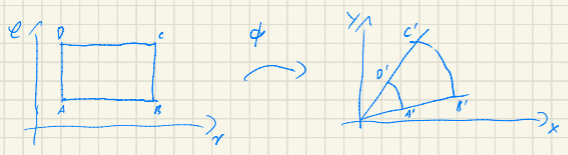
\includegraphics[height=2cm]{img/VII_Bsp_1_Polarkoordinaten.png}
    \end{center}
  \end{example}

  \begin{remark}[Notation]
    $x \in \mathbb{R}^n, \delta >0$\\
    $Q(x, \delta) = \{y \in \mathbb{R}^n \ | \ ||y-x||_{\infty} \leq \delta\}, ||x||_{\infty} = \max\limits_{1 \leq k \leq n} | x_k |$
    \begin{center}
      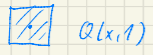
\includegraphics[height=1cm]{img/VII_Notation_1_Qx1.png}
    \end{center}
  \end{remark}

  \begin{lemma}
    Sei $\script{U} \subseteq \mathbb{R}^n$ offen, $x_0 \in \script{U}$ und $\Phi: \script{U} \to \mathbb{R}^n$ mit $D\Phi(x_0) \in GL_n(\mathbb{R})$. Gegeben sei eine Folte $Q_j = Q(x_j, \phi_j)\subseteq \script{U}$ mit $\phi_j \to 0$ und $x_0 \in Q_j \ \forall \ j \in \mathbb{N}$. Dann gilt:
    $$\limsup\limits_{j \to \infty} \frac{\lambda^n(\Phi(Q_j))}{\lambda^n(Q_j)} \leq |det D\Phi(x_0)|$$
  \end{lemma}
  \begin{proof}
    siehe Aufschrieb
  \end{proof}

  \begin{theorem}[Transformationsformel]
    $\script{U}, \script{V} \subseteq\mathbb{R}^n$ offen, $\Phi:\script{U} \to \script{V} C^1$-Diffeomorphismus. Ist $A \subseteq \script{U}$ $\lambda^n$-messbar, so ist auch $\Phi(A)$ $\lambda^n$-messbar und es gilt:
    \begin{enumerate}
      \item $\lambda^n(\Phi(A)) = \int\limits_A | \det D\Phi(x) | dx$
    \end{enumerate}
    Weiter gilt für jede $\lambda^n$-messbare Funktion $f: \script{V} \to \bar{\mathbb{R}}$:
    \begin{enumerate}[resume]
      \item $\int\limits_{\script{V}} f(y) dy = \int\limits_{\script{U}} f(\Phi(x)) |\det D\Phi(x)| dx \ \ (dy \ \hat{=} \ d\lambda^n(y))$
    \end{enumerate}
    falls eines der Integrale definiert ist.
  \end{theorem}

  \begin{proof}
    siehe Aufschrieb
  \end{proof}

  \sidenote{Vorlesung 20}{22.01.2021}
  \begin{example}
    \begin{enumerate}
      \item[]
      \item
        \begin{align*}
          f:\mathbb{R}^2 \to \mathbb{R}, f(x,y) = e^{-(x^2+y^2)} = e^{-||(x,y)||^2}\\
          \int\limits_{\mathbb{R}^2} f d\lambda^2 \stackrel{\text{Fubini}}{=} \int\limits_{\mathbb{R}} e^{-x^2}(\int\limits_{\mathbb{R}} e^{-y^2} dy) dx = (\int\limits_{\mathbb{R}}^{-x^2} dx)^2
        \end{align*}
        Für Polarkoordinaten $\Phi:(0,\infty) \times (0,2\pi) \to \mathbb{R}^2 \setminus \{(x,0) \ | \ x \geq 0\}$ gilt: \\
        $$\det D\Phi(r,\Theta) = r$$\\
        Da $\{(x,0) \ | \ x \geq 0\}$ eine $\lambda^2$-Nullmenge ist, folgt aus der Transformationsformel:
        \begin{align*}
          \int\limits_{\mathbb{R}^2} f d\lambda^2
          &= \int\limits_{(0,\infty) \times (0,2\pi)} e^{-r^2} d\lambda^2(r,\Theta)\\
          &\stackrel{\text{Fubini}}{=} \int\limits_0^{\infty} e^{-r^2}r(\int\limits_0^{2\pi}d\Theta)dr\\
          &= 2\pi \int\limits_0^{\infty} e^{-r^2} r dr\\
          &= 2\pi [-\frac{1}{2} e^{-r^2}]_{r=0}^{r=\infty}\\
          &= \pi\\
          \implies \int\limits_0^{\infty} e^{-x^2} dx &= \sqrt{x}
        \end{align*}
      \item Spezialfall $\Phi: \script{U} \to \script{V} C^1$-Diffeomorphismus ist Einschränkung einer linearen Abbildung.
        \begin{align*}
          &\implies \Phi(x) = Sx \text{ mit } S\in GL_n(\mathbb{R})\\
          &\implies D\Phi(x) = S \ \forall \ x \in \script{U}\\
          &\stackrel{Trafo}{\implies} \lambda^n(S(D)) = |\det S| \lambda^n(D) \text{ (siehe Satz ???)}\\
          \text{bzw. } \int\limits_{\script{V}} f(y) d\lambda^n(y) &= |\det S| \int\limits_{\script{U}} f(Sx) d\lambda^n(x)
        \end{align*}
      \item Polarkoordinaten im $\mathbb{R}^3$\\
        $$\Phi(r, \Theta, \phi) = (r \sin(\Theta) \cos(\phi), r \sin(\Theta)\sin(\phi), r \cos(\Theta))$$ ist $C^{\infty}$-Diffeomorphismus der offenen Mengen $\script{U} = (0,\infty) \times (0,\pi) \times (0,2\pi)$ und $\script{V} = \mathbb{R}^3 \setminus \{(x,0,z) \ | \ x \geq 0\}$\\
        Inverse:\\
        $r=\sqrt{x^2 + y^2 + z^2}, \Theta = \arccos(\frac{z}{r})$\\
        $\phi = \begin{cases}
          \arccos(\frac{x}{\sqrt{x^2 + y^2}}) & \text{, für } y \geq 0\\
          2\pi - \arccos(\frac{x}{\sqrt{x^2 + y^2}}) & \text{, für } y \leq 0
        \end{cases}$\\
        $D\Phi(r, \Theta, \phi) = \left(\begin{array}{ccc}
          \sin(\Theta)\cos(\phi) & r\cos(\Theta)\cos(\phi) & -r\sin(\Theta)\sin(\phi)\\
          \sin(\Theta)\sin(\phi) & r\cos(\Theta)\sin(\phi) & r\sin(\Theta)\cos(\phi)\\
          \cos(\Theta) & -r\sin(\Theta) & 0
        \end{array} \right)$
        \begin{align*}
          &\implies \det D\Phi = r^2 \sin(\Theta)\\
          E &:= [r_1, r_2] \times [\Theta_1, \Theta_2] \times [\phi_1, \phi_2]\\
          \lambda^3(\Phi(E)) &= \int\limits_{r1}^{r2}\int\limits_{\Theta_1}^{\Theta_2}\int\limits_{\phi_1}^{\phi_2} r^2 \sin(\Theta) d\phi d\Theta dr = \frac{r_2^3 - r_1^3}{3} (\cos(\Theta_1) - \cos(\Theta_2)) (\phi_2 - \phi_1)
        \end{align*}
    \end{enumerate}
  \end{example}

  \begin{remark}
    \underline{Ziel:} Umrechnung von Differentialoperatoren\\
    Begriff: $\Phi: \script{U} \to \script{V} C^k$-Diffeomorphismus zwischen $\script{U}, \script{V}$ offen.\\
    Gramsche Matrix $g \in C^{k-1}(\script{U}, \mathbb{R}^{n\times n}), g = (g_{i,j})$
    $$g(x) = D\Phi(x)^{\top} D\Phi(x) \text{ bzw.}\\
    g_{i,j}(x) = <\frac{\partial\Phi}{\partial x_i}(x), \frac{\partial\Phi}{\partial x_j}(x)>$$\\
    Für Polarkoordinaten im $\mathbb{R}^3$ gilt:
    $$(g_{i,j}(r, \Theta, \phi))_{1\leq i,j \leq 3} = \left(\begin{array}{ccc}
      1 & 0 & 0 \\
      0 & r^2 & 0 \\
      0 & 0 & r^2 \sin^2(\Theta)      
    \end{array}\right)$$
    
    \newpage

    Allgemein gilt:\\
    $g(x)$ ist symmetrisch und strikt positiv definit, denn
    $$<g(x)v,v> \ = \ <D\Phi(x)^{\top}D\Phi(x) v, v> \ = |D\Phi(x) v|^2 > 0$$
    für $v\neq 0$ und $D\Phi(x) \in GL_n(\mathbb{R}) \implies g(x)$ ist invertierbar.\\
    \\
    Wir setzen: $g^{ij}(x) = (g(x)^{-1})_{ij}$\\
    ... (Rest siehe Aufschrieb)
  \end{remark}

  \begin{theorem}
    Sei $\Phi \in C^1(\script{U}, \script{V})$ Diffeomorphismus zwischen $\script{U}, \script{V} \subseteq \mathbb{R}^n$ offen mit gramscher Matrix $(g_{ij})$
    \begin{enumerate}
      \item Für $v \in C^1(\script{V})$ gilt mit $\mu = v \circ \Phi$:
      $$(\triangledown v) \circ \Phi = D\Phi \cdot \triangledown_g u \ \ , \ \ \triangledown_g u := \sum\limits_{i,j=1}^n g^{ij} \frac{\partial u}{\partial x_i} e_j$$
      \item Für $y \in C^1(\script{V}, \mathbb{R}^n)$ gilt mit $y \circ \Phi = D\Phi x$:
        $$(div(y)) \circ \Phi = div_g x := \frac{1}{\sqrt{det(g)}} \sum\limits_{j=1}^n \frac{\partial}{\partial x_j} (\sqrt{det(g)} x_j)$$
      \item Ist $\Phi \in C^2(\script{U}, \script{V}), v \in C^2(\script{V}), u = v \circ \Phi$
        $$\implies (\triangle v) \circ \Phi = div_g \triangledown_g u = \frac{1}{\sqrt{det(g)}} \sum\limits_{i,j=1}^n \frac{\partial}{\partial x_i} (\sqrt{det(g)} g^{ij} \frac{\partial u}{\partial x_j})$$
    \end{enumerate}
  \end{theorem}
  \begin{proof}
    siehe Aufschrieb
  \end{proof}

  \begin{example}[Laplace in Polarkoordinaten im $\mathbb{R}^3$]
    \begin{align*}
      \triangledown_g u &= \frac{\partial u}{\partial r} e^r + \frac{1}{r^2} \frac{\partial u}{\partial \Theta} e^{\Theta} + \frac{1}{r^2 \sin^2(\Theta)} \frac{\partial u}{\partial \phi} e^{\phi}\\
      div_g x &= \frac{1}{r^2} \frac{\partial}{\partial r} (r^2 x^r) + \frac{1}{\sin(\Theta)} \frac{\partial}{\partial \Theta} (\sin(\Theta) x^{\Theta}) + \frac{\partial x^{\phi}}{\partial \phi}\\
      \triangle_g u &= \frac{1}{r^2} \frac{\partial}{\partial r} (r^2 \frac{\partial u}{\partial r})  + \frac{1}{r^2 \sin(\Theta)} \frac{\partial}{\partial \Theta} (\sin(\Theta) \frac{\partial u}{\partial \Theta}) + \frac{1}{r^2 \sin^2(\Theta)} \frac{\partial^2 u}{\partial \phi^2}
    \end{align*}
    $e^r, e^{\Theta}, e^{\phi}$ Standardbasis im $(r, \Theta, \phi)$-Raum und $x^r, x^{\Theta}, x^{\phi}$ sind zugehörige Koordinaten
    $$v(x,y,z) = (x^2 + y^2 + z^2)^{-\frac{1}{2}} \implies u = r^{-1}$$
    $$\implies \triangle v\circ \Phi = \triangle_g u = 0 \text{ auf }\mathbb{R}^3\setminus\{0\}$$
  \end{example}
  \chapter{Das Flächenmaß auf Untermannigfaltigkeiten}
  \sidenote{Vorlesung 21}{25.01.2021}

  \begin{definition}
    Sei $\script{U} \subseteq \mathbb{R}^n$ offen. Eine Abbildung $f \in C^1(\script{U}, \mathbb{R}^{n+k})$ heißt \textbf{Immersion}, wenn gilt:
    $$Rang \ Df(x) = n \Leftrightarrow Ker \ Df(x) = \{0\} \ \forall \ x \in \script{U}$$
    $\frac{\partial f}{\partial x_1}(x), ..., \frac{\partial f}{\partial x_n}(x)$ bilden eine Basis von $Bild \ Df(x) \subseteq \mathbb{R}^{n+k}$. $n$ heißt \textbf{Dimension}, $k$ die \textbf{Kodimension} von $f$.\\
    Wir definieren die \textbf{Gramsche Matrix} oder \textbf{induzierte Metrik}
    $$g(x) = Df(x)^{\top} Df(x)$$ 
    $$\text{bzw. } g_{ij}(x) = <\frac{\partial f}{\partial x_i}|x|, \frac{\partial f}{\partial x_j}|x|>$$
    $\rightarrow (g_{ij})$ ist für $f \in C^1(\script{U}, \mathbb{R}^{n+k})$ beliebig definiert und positiv semidefinit.\\
    Die Matrix ist genau dann strikt positiv definit und damit invertierbar, wenn $f$ eine Immersion ist:
    $$<g(x)v, v> = |Df(x)v|^2 \geq 0$$
    $$\implies Ker \ g(x) = Ker \ Df(x)$$
  \end{definition}

  \begin{definition}{Flächenformel}
    $\script{U} \subseteq \mathbb{R}^n$ offen, $f \in C^1(\script{U}, \mathbb{R}^{n+k})$ eine $n$-dimensionale Immersion mit Gramscher Matrix $g$, und $E \subseteq \script{U}$ sei $\lambda^n$-messbar.\\
    Der ($n$-dimensionale) \textbf{Flächeninhalt} von $f$ auf $E$ ist definiert durch
    $$A(f,E) = \int\limits_E Jf(x) \ dx$$
    $$\text{mit } Jf = \sqrt{det \ g}$$
    $Jf$ heißt \textbf{Jacobische} von $f$.
  \end{definition}

  \newpage
  \begin{example}
    \begin{enumerate}
      \item[]
      \item $f = S \circ \Phi: \script{U} \to \mathbb{R}^{n+k}, \Phi \in C^1(\script{U}, \script{V})$ Diffeomorphismus zwischen $\script{U}, \script{V} \subseteq \mathbb{R}^n$ offen und $S: \mathbb{R}^n \to Y \subseteq \mathbb{R}^{n+k}$ lineare Isometrie, $E \subseteq \script{U}$ messbar, $Df(x) = S \ D\Phi(x)$
        \begin{align*}
          \implies A(f,E) 
          &= \int\limits_E \sqrt{det \ D\Phi(x)^{\top} S^{\top} S D\Phi(x)} dx\\
          &= \int\limits_E |det \ D\Phi(x)| dx \stackrel{Trafo}{=} \lambda^n(\Phi(E))
        \end{align*}
      \item 1-dim Immersion $f: I = (a,b) \to \mathbb{R}^n \ f=f(A)$ heißt \textbf{reguläre Kurve} Gramscher Matrix $g_{11}=<f'(A), f'(A)> = ||f'(A)||^2$\\
        Länge von Kurve $\rightarrow L(f) = \int\limits_a^b ||f'(A)|| dt$\\
        $$f(A) = (cos(t), sin(t)) \ \ \ L(f, [0, 3\pi]) = 3\pi$$
      \item 2-dim Immersion in $\mathbb{R}^n \ (n=2, k=1) \ f:\script{U}\to\mathbb{R}^3, f=f(x,y)$ heißt \textbf{reguläre Fläche}
        $$(g_{ij}) = \begin{pmatrix}
          ||\frac{\partial f}{\partial x}||^2 & <\frac{\partial f}{\partial x}, \frac{\partial f}{\partial y}>\\
          <\frac{\partial f}{\partial x}, \frac{\partial f}{\partial y}> & ||\frac{\partial f}{\partial y}||^2
        \end{pmatrix}$$ 
        $\implies Jf = \sqrt{||\frac{\partial f}{\partial x}||^2 ||\frac{\partial f}{\partial y}||^2 - <\frac{\partial f}{\partial x}, \frac{\partial f}{\partial y}>^2} = ||\frac{\partial f}{\partial x} \times \frac{\partial f}{\partial y}||$\\
        $(||a||^2||b||^2-<a,b>^2 = ||a \times b||^2 \text{ siehe LA})$\\
        \begin{align*}
          &\text{Polarkoordinaten:}\\
          &f: \script{U} = (0, \pi) \times (0, 2\pi) \to S^2\subseteq \mathbb{R}^3\\
          &f(\theta, \phi) = \begin{pmatrix}
            sin(\theta)cos(\phi) & sin(\theta)sin(\phi) & cos(\theta)
          \end{pmatrix}\\
          &\stackrel{\text{Kap. VII}}{\implies} Jf(\theta, \phi) = sin(\theta) \implies f \text{ reguläre Fläche}\\
          &A(f) = \int\limits_0^{\pi}\int\limits_0^{2\pi} sin(\theta) \ d\phi \ d\theta = 4\pi
        \end{align*}
      \item siehe Aufschrieb
    \end{enumerate}
  \end{example}

  \begin{theorem}
    $\Phi \in C^1(\script{U}, \script{V})$ Diffeomorphismus, $\script{U}, \script{V} \subseteq \mathbb{R}^n$ offen und $f \in C^1(\script{V}, \mathbb{R}^{n+k})$ Immersion. Dann gilt:
    $$A(f, \Phi(E)) = A(f\circ\Phi, E) \ \ \ \forall \ E \subseteq \script{U} \ \lambda^n\text{-messbar}$$
  \end{theorem}
  \begin{proof}
    siehe Aufschrieb
  \end{proof}

  \begin{definition}[Untermannigfaltigkeiten]
    Eine Menge $M \subseteq \mathbb{R}^{n+k}$ heißt \textbf{Untermannigfaltigkeit} des $\mathbb{R}^{n+k}$, der Klasse $C^r,\\ r\in \mathbb{N}\cup\{\infty\}$ offen (mit $M \in \Omega$) und $\exists \ \Phi: \Omega \to \Phi(\Omega) \\
    C^r$-Diffeomorphismus mit
    $$\Phi(M \cap \Omega) = (\mathbb{R}^n \times \{0\}) \cap \Phi(\Omega)$$
    ($\Phi$ heißt \textbf{lokale Plättung} von $M$)\\
    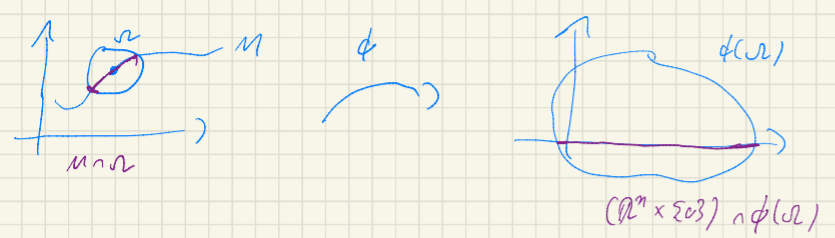
\includegraphics[width=\textwidth]{img/VIII_4_UnterMGF.png}
  \end{definition}

  \begin{theorem}
    Sei $M \subseteq \mathbb{R}^{n+k}$. Dann sind äquivalent:
    \begin{enumerate}
      \item $M$ ist $n$-dimensionale Untermannigfaltigkeit der Klasse $C^r$
      \item $\forall p \in M \ \exists \ \Omega\subseteq\mathbb{R}^{n+k}$ offene Umgebung vvon $p$ und $f \in C^r(\Omega, \mathbb{R}^k)$ mit $M \cap \Omega = f^{-1}(0)$ und $Rang \ Df = k$ auf $\Omega$
      \item $\forall p \in M \ \exists$ offene Umgebungen $\script{U}\subseteq \mathbb{R}^n, V\subseteq \mathbb{R}^k$ und $g \in C^r(\script{U}, \script{V})$, so dass nach geeigneter Permutation der Koordinaten gilt:\\
      $$M \cap (\script{U} \times \script{V}) = \{(x, g(x)) \ | \ x \in \script{U}\}$$
      \item $\forall p \in M \ \exists$ offene Umgebung $\script{U}\subseteq \mathbb{R}^n$ und $\script{C} \in C^r(\script{U}, \mathbb{R}^{n+k})$ mit $\script{C}(x_0) = p$ für ein $x_0 \in \script{U}$ und $Rang \ D\script{C}(x) = n \ \forall \ x\in M$, so dass $\script{C}$ offene Teilmengen von $\script{U}$ in relativ offene Teilmengen von $M$ abbildet. 
    \end{enumerate}
  \end{theorem}

  \sidenote{Vorlesung 22}{29.01.2021}

  \begin{theorem}
    Jede $n$-dimensionale Untermannigfaltigkeit $M \subseteq \mathbb{R}^{n+k}$ ist als abzählbare Vereinigung $M = \bigcup\limits_{i\in\mathbb{N}} K_i$ von kompakten Mengen darstellbar.
  \end{theorem}
  \begin{proof}
    siehe Aufschrieb
  \end{proof}

  \begin{definition}
    Sei $M \subseteq \mathbb{R}^{n+k}$ eine $n$-dimensionale Untermannigfaltigkeit der Klasse $C^1$. Eine \textbf{lokale Parametrisierung} von $M$ ist eine injektive Immersion $f: \script{U} \to M \subseteq \mathbb{R}^{n+k}$, wobei $M \subseteq \mathbb{R}^n$ offen und $f \in C^1$.
  \end{definition}

  \begin{lemma}
    Für jede Untermannigfaltigkeit $M \subseteq \mathbb{R}^{n+k}$ der Klasse $C^1$ gibt es lokale\\
    $C^1$-Parametrisierungen $f_i:\script{U}_i \to M$, wobei $i\in\mathbb{N}$, sodass $M = \bigcup\limits_{i \in \mathbb{N}} f_i(\script{U}_i)$
  \end{lemma}
  \begin{proof}
    siehe Aufschrieb
  \end{proof}

  \begin{theorem}
    $M \subseteq \mathbb{R}^{n+k}$ $C^1$-Untermannigfaltigkeit. Dann gelten:
    \begin{enumerate}
      \item Ist $f: \script{U} \to M$ lokale Parametrisierung von $M$, so ist $f(\script{U})$ offen in $M$ und $f: \script{U} \to f(\script{U})$ ist homeomorph, d.h. $f^{-1}$ ist stetig bzgl. euklidischer Metrik auf $f(\script{U})$.
      \item Sind $f_i:\script{U}_i \to f(\script{U}_i) = \script{V}_i$ für $i = 1,2$ lokale $C^1$-Parametrisierung von $M$, so ist $f_2^{-1}\circ f_1: f_1^{-1}(\script{V}_1\cap\script{V}_2) \to f_2^{-1}(\script{V}_1\cap\script{V}_2)$ ein $C^1$-Diffeomorphismus. 
    \end{enumerate}
  \end{theorem}
  \begin{proof}
    siehe Aufschrieb
  \end{proof}

  \begin{theorem}[Flächenmaß]
    $M \subseteq \mathbb{R}^{n+k} C^1$-Untermannigfaltigkeit. Dann heißt $E \subseteq M$ messbar, falls gilt:
    $$f^{-1}(E) \text{ ist } \lambda^n\text{-messbar für jede lokale Parametrisierung } f: \script{U} \to M$$
    Das System $\script{M}$ der messbaren Teilmengen von $M$ ist eine $\sigma$-Algebra. Diese enthält die Borelmengen in $M$. Weiter gibt es genau ein Maß $\mu_M$ auf $\script{M}$, so dass für jede lokale Parametrisierung $f: \script{U} \to M$ und jedes $E \subseteq f(\script{U})$ messbar gilt:
    $$\mu_M(E) = \int\limits_{f^{-1}(E)}Jf(x) \ dx$$
  \end{theorem}
  \begin{proof}
    siehe Aufschrieb
  \end{proof}

  \newpage
  \begin{theorem}[Oberflächenintegral]
    Sei $M \subseteq \mathbb{R}^{n+k} n$-dimensionale $C^1$-Untermannigfaltigkeit und $M = \bigcup\limits_{i \in \mathbb{N}} M_i$ eine paarweiße disjunkte, messbare Zerlegung mit $M_i \subseteq \script{V}_i$ für lokale Parametrisierungen $f_i: \script{U}_i \to \script{V}_i$. Für eine messbare Funktion $u: M \to \bar{\mathbb{R}}$ gilt:
    $$\int\limits_M u \ d\mu_M = \sum\limits_{i \in \mathbb{N}} \int\limits_{f_i^{-1}(M_i)} u(f_i(x))\ Jf_i(x)\ dx$$
  \end{theorem}

  \sidenote{Vorlesung 23}{01.02.2021}
  \begin{lemma}
    Sei $T:\mathbb{R}^{n+k} \to \mathbb{R}^{n+k}$ eine \textbf{Ähnlichkeitsabbildung}, d.h. $\exists \lambda>0, Q\in O(n+k)$ und $a\in\mathbb{R}^{n+k}$ mit $T(p) = \lambda Q(p+a)$. Ist $M \subseteq \mathbb{R}^{n+k}$ eine $n$-dimensionale $C^1$-Untermannigfaltigkeit, so auch $N = T(M)$ und für $\mu_M$ bzw. $\mu_N$ gilt:
    \begin{enumerate}
      \item Ist $A \subseteq M$ messbar $\implies T(A) \subseteq N$ messbar und 
        $$\mu_N(T(A)) = \lambda^n (\mu_M(A))$$
      \item Ist $u: N \to \bar{\mathbb{R}} \ \mu_N$-messbar, so ist $u \circ T: M \to \bar{\mathbb{R}} \ \mu_M$-messbar und es gilt, sofern eines der Integrale existiert:
        $$\int\limits_N u(q) \ d\mu_N(q) = \lambda^n \int\limits_M u(T(p)) \ d\mu_M(p)$$
    \end{enumerate}
  \end{lemma}
  \begin{proof}
    siehe Aufschrieb
  \end{proof}

  \begin{theorem}[Zwiebelformel]
    Für $u \in L^1(\mathbb{R}^{n+1})$ ist $u|_{\partial B_r(0)} \subseteq L^1(\mu_{\partial B_r(0)})$ für fast alle $r>0$ und es gilt:
    \begin{align*}
      \int\limits_{\mathbb{R}^{n+1}} u(p) \ dp
      &= \int\limits_0^{\infty} \int\limits_{\partial B_r(0)} u(p) \ d\mu_{\partial B_r(0)}(p)\ dr\\
      &= \int\limits_0^{\infty} r^n \int\limits_{S^n} u(rw) \ d\mu_{S^n}(w)\ dr
    \end{align*}
  \end{theorem}
  \begin{proof}
    siehe Aufschrieb
  \end{proof}

  \newpage
  \begin{example}
    Mit $u = \psi_{B_1(0)}$ folgt für $w_n = \mu_{S^n}(S^n)$:
    $$\alpha_{n+1} = \lambda^{n+1}(B_1(0)) = \int\limits_0^1 \mu_{\partial B_r(0)} (\partial B_r(0)) \ dr = \int\limits_0^1 w_n r^n \ dr = \frac{w_n}{n+1}$$
    $\implies w_n = (n+1) \alpha_{n+1}$\\
    z.B. $w_1 = 2\pi, w_2 = 4\pi, w_3 = 2\pi^2, ...$
  \end{example}
  \chapter{Der Integralsatz von Gauß}

(Einleitung siehe Aufschrieb)

\begin{theorem}
  Für $\Omega \subseteq \mathbb{R}^n$ offen sind äquivalent:
  \begin{enumerate}
    \item Plättung:\\
      $\forall \ p \in \partial \Omega \ \exists \ W \subseteq \mathbb{R}^n$ offen mit $p \in W$ und $\Phi: W\to \Phi(W)$\\
      $C^1$-Diffeomorphismus mit:
      $$\Phi(W \cap \Omega) = \mathbb{H}^n \cap \Phi(W) \text{ wobei } \mathbb{H}^n = \mathbb{R}^{n-1} \times (-\infty, 0)$$
      \includegraphics[width=.8\textwidth]{img/IX_1_Plättung.png}
    \item Subniveau:\\
      $\forall p\in \partial \Omega \ \exists W \subset \mathbb{R}^n$ offen mit $p \in W$ und $h \in C^1(W)$ mit $Dh(q) \neq 0) \\\forall q \in W$, sodass $\Omega \cap W = \{q \in W \ | \ h(q) < 0\}$
    \item Subgraph:\\
      $\forall p \in \partial\Omega \ \exists \script{U} \subseteq \mathbb{R}^{n-1}$ offen $\exists$ offenes Intervall $I \subseteq \mathbb{R} \ \exists C^1$-Funktion $u: \script{U} \to I$, sodass nach geeigneter Umnummerierung der Koordinaten gilt:
      $$\Omega \cap (\script{U} \times I) = \{(x,y) \in \script{U} \times I \ | \ y < u(x)\}$$
  \end{enumerate}
  Die Menge $\Omega$ hat $C^1$-Rand wenn eines (und damit jedes) der drei Kriterien erfüllt ist.
\end{theorem}
\begin{proof}
  siehe Aufschrieb
\end{proof}

\newpage
\begin{lemma}
  In der Situation von Satz IX.1,3) gilt:
  \begin{align*}
    \partial \Omega \cap(\script{U}\times I) &= \{(x,y) \in \script{U} \times I \ | \ y = u(x)\}\\
    (\mathbb{R}\setminus \bar{\Omega}) \cap (\script{U}\times I) &= \{(x,y) \in \mathbb{U} \times I \ | \ y > u(x)\}
  \end{align*}
  $\implies \partial \Omega$ ist $(n-1)$-dimensionale $C^1$-Untermannigfaltigkeit des $\mathbb{R}^n$ nach dem Graphenkriterium bei Untermannigfaltigkeiten.
\end{lemma}
\begin{proof}
  siehe Aufschrieb
\end{proof}

\sidenote{Vorlesung 24}{05.02.2021}
\begin{lemma}
  $\Omega \subseteq \mathbb{R}^n$ offen mit $C^1$-Rand. Dann gibt es zu $p \in \partial\Omega$ genau einen Vektor $\nu(p)\in \mathbb{R}^n$ mit
  \begin{enumerate}
    \item $\nu(p) \perp T_p(\partial \Omega)$ und $||\nu(p)|| = 1$
    \item $p + t \nu(p) \notin \Omega$ für $t$ hinreichend klein
  \end{enumerate}
  $\nu:\partial\Omega\to\mathbb{R}^n, n \mapsto \nu(p)$ ist stetig und heißt \textbf{äußere Normale} von $\Omega$.
\end{lemma}

\begin{remark}[Erinnerung: Tangentialraum]
  $\nu \in \mathbb{R}^n$ heißt \textbf{Tangentialvektor} von $M \subseteq R^n, C^1$-Untermannigfaltigkeit in $p\in M$, falls $\gamma:(-\delta, \delta) \to M$ existiert mit $\gamma(0) = p, \gamma'(0) = \nu$\\
  $T_pM = \{$Alle Tangentualvektoren$\}$ $(n-1)$-dimensionaler Untervektorraum.
\end{remark}

\begin{definition}
  Für $\Omega \subseteq \mathbb{R}^n$ sei $C^1(\bar{\Omega})$ der Unterraum aller $f\in C^1(\Omega)$, für die $f$ und $Df$ stetige Fortsetzungen auf $\partial \Omega$ besitzen. Die \textbf{Fortsetzung} wird wieder mit $f$ bezeichnet.
\end{definition}

\begin{lemma}
  Sei $\Omega = \{(x,y) \in \script{U} \times T \ | \ y<u(x)\}$ wobei $\script{U} \subseteq \mathbb{R}^{n-1}$ offen, $I = (a,b) \subseteq \mathbb{R}$ und $u \in C^1(\script{U}, I)$. Hat $X \in C^1(\bar{\Omega, \mathbb{R}^n})$ kompakten Träger in $\script{U}\times I$, so gilt:
  $$\int\limits_{\Omega} div \ X \ d\lambda^n = \int\limits_{\partial \Omega} <X, \nu> \ d\mu$$
\end{lemma}
\begin{proof}
  siehe Aufschrieb
\end{proof}

\begin{lemma}
  Sei $W_{\lambda}, \lambda \in \Lambda$, eine offene Überdeckung der kompakten Menge $K \subseteq \mathbb{R}^n$. Dann gibt es eine \textbf{untergeordnete Teilung der Eins}, d.h. es gibt eine endliche Familie von Funktionen $\psi_j \in C_c^{\infty}(\mathbb{R}^n), j \in J$, so dass gilt:
  \begin{enumerate}
    \item $\sum\limits_{j \in J} \psi_j(p) = 1 \ \ \ \forall \ p \in K$
    \item $\forall \ j \in J \ \exists \ \lambda = \lambda(j)$ mit $spt \ \psi_j \subseteq W_{\lambda}$
  \end{enumerate}
\end{lemma}
\begin{proof}
  siehe Aufschrieb
\end{proof}

\begin{theorem}[Integralsatz von Gauß]
  $\Omega \subseteq \mathbb{R}^n$ offen, beschränkt mit $C^1$-Rand und äußere Normale $\nu:\partial\Omega\to\mathbb{R}^n$. Dann gilt für $X\in C^1(\bar{\Omega}, \mathbb{R}^n)$:
  $$\int\limits_{\Omega} div \ X \ d\lambda^n = \int\limits_{\partial\Omega} <X, \nu> \ d\mu$$
\end{theorem}
\begin{proof}
  siehe Aufschrieb
\end{proof}

\begin{remark}
  Gilt auch für Gebiete, deren Rand lokal lipschitz ist (d.h. $u$ in Satz IX.1,3) ist lipschitz (siehe Buch von H.W. Alt: Lineare Funktionalanalysis) \\
  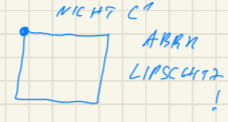
\includegraphics[width=3cm]{img/IX_7_Bem.png}
\end{remark}

\sidenote{Vorlesung 25}{08.02.2021}
\begin{example}
  Wähle $X(x) = x \implies \lambda^n(\Omega) = \frac{1}{n} \int\limits_{\Omega} div \ X \ dx = \frac{1}{n} \int\limits_{\partial \Omega} <x, \nu(x)> \ d\mu(x)$\\
  Speziell: $\alpha = \frac{\omega_{n-1}}{n}$\\
  $\Omega = B_1(0) \subseteq \mathbb{R}^n \rightarrow \nu(x) = x, \partial\Omega = S^{n-1}$ 
\end{example}

\newpage
\begin{lemma}[Greensche Formeln]
  $\Omega \subseteq \mathbb{R}^n$ offen und beschränkt mit $C^1$-Rand. Dann gilt für $u \in C^1(\bar{\Omega})$ und $v \in C^2(\bar{\Omega})$
  \begin{enumerate}
    \item $\int\limits_{\Omega}(u \triangle v + <\triangledown u, \triangledown v>) \ d\lambda^n = \int\limits_{\partial \Omega} u \frac{\partial v}{\partial \nu} \ d\mu \ \ \ (\frac{\partial v}{\partial \nu} = <\triangledown v, \nu>)$
  \end{enumerate}
  Weiter folgt für $u,v \in C^2(\bar{\Omega})$
  \begin{enumerate}[resume]
    \item $\int\limits_{\Omega} (u \triangle v - v \triangle u) \ d\lambda^n = \int\limits_{\partial \Omega}(u \frac{\partial v}{\partial \nu} - v \frac{\partial u}{\partial \nu}) \ d\mu$
  \end{enumerate}
\end{lemma}

\begin{proof}
  siehe Aufschrieb
\end{proof}

\begin{example}
  \underline{Mittelwerteigenschaft harmonischer Funktionen}\\
  Sei $\mu \in C^2(\Omega)$ eine \textbf{harmonische Funktion}, d.h. $\triangle u = 0$ in $\Omega$.\\
  Für $x_0 \in \Omega$ und $0<r<dist(x_0, \partial \Omega)$ gilt:
  $$\int\limits_{\partial B_r(x_0)} \frac{\partial u}{\partial \nu} \ d\mu \stackrel{\text{Gauß}}{=} \int\limits_{B_r(x_0)} \triangle u \ d\lambda^n = 0 \ \ \ \ \ \triangle u = div \ (\triangledown u)$$
  Auf $\mathbb{R}^n\setminus\{x_0\}$ betrachte weiter $v(x) = \gamma(||x-x_0||)$ mit $\gamma(\rho) = \begin{cases}
    \frac{\rho^{2-n}}{2-n} & , n\geq 3\\
    \log(\rho) & , n = 2
  \end{cases}$\\
  $\stackrel{\text{Ana II}}{\implies} v$ ist harmonisch auf $\mathbb{R}^n\setminus\{x_0\}$\\
  \\
  ... Rest siehe Aufschrieb
\end{example}

\begin{example}
  siehe Aufschrieb
\end{example}
  
\end{document}